\chapter{Úvod}
\label{uvod}
Nejpopulárnějším způsobem modelování a reprezentace dat pro vykreslování je v~současné době využití trojúhelníkových sítí, ale existují i další přístupy. Jednou z~poměrně populárních alternativ je využití voxelů. I~přes to, že voxelové reprezentace jsou v~real-time grafice v~menšině, lze nalézt spoustu zdrojů a vědeckých článků o~této problematice.

Vzhledem ke změnám možností využití grafické karty, především existenci compute shaderů, je práce s~voxely mnohem jednodušší, než tomu bylo v~dřívějších dobách. Není nutné provádět převod na trojúhelníky a můžeme pracovat s~voxelovými primitivy přímo. Tím se odemyká možnost využití optimalizovaných algoritmů. Tato práce se zabývá zobrazováním voxelových scén za pomocí moderních metod a nástrojů, které jsou vývojářům poskytnuty.

Cílem této práce je navrhnout a implementovat systém pro vykreslování voxelových scén. Z mnoha dostupných metod jsou zde využity dvě -- sparse voxel octree ray tracing z článku \cite{Laine2011EfficientSV} a light field probes z článku \cite{light_field_probes}. Pro light field probes byla vytvořena vlastní modifikace k výpočtu a vykreslení nepřímého osvětlení ve scéně.

První kapitola si dává za cíl seznámit čtenáře s~řešenou problematikou. Vysvětluje základní principy realistického zobrazování a některé populární metody, jimiž je toho možné dosáhnout. Také popisuje, co jsou voxely, jak se s~nimi dá pracovat v~kontextu rozdělení prostoru a základní metody vykreslování. Dále jsou zde popsány vybrané hierarchické struktury, pomocí kterých lze urychlit průchod voxelovým prostorem. V~poslední řadě obsahuje krátký popis moderního API pro práci s~grafickými kartami: Vulkan.

Kapitola druhá se zabývá návrhem řešení. Je zde popsán způsob reprezentace voxelových dat s~využitím akcelerační struktury a její detaily. Kapitola také vysvětluje navrhovaný způsob vykreslování voxelových scén s~využitím ray casting přístupu pro primární paprsky a představuje způsob výpočtu nepřímého osvětlení za pomocí sond. V poslední části je vysvětleno jak do sebe jednotlivé části zapadají ve větším celku.

Následující kapitola se zabývá specifikami implementace. V~prvé radě jsou uvedeny nástroje a knihovny využité v~samotné implementaci. Dále jsou popsány knihovny, které byly v~rámci práce vytvořeny: knihovna obsahující obecné nástroje, knihovna pro usnadnění práce s~Vulkan a GLFW, a knihovna pro vytváření a interakci s~uživatelským rozhraním. Také je zde popsána základní struktura výsledného programu společně se specifikami implementace jako je transformace modelů či správa modelů v paměti. Poslední sekce krátce popisuje uživatelské rozhraní demonstrační aplikace.

Poslední kapitola se věnuje vyhodnocením dosažených výsledků. Obsahem je analýza doby převodu scén do interní reprezentace, paměťová náročnost využitých datových struktur a také vyhodnocení dosažených grafických výstupů implementace.

\chapter{Teorie}
\label{teorie}
Cílem této kapitoly je seznámit čtenáře s~koncepty nutnými pro pochopení vlastního řešení. Kapitola nejprve definuje a vysvětluje, co je to voxel a jaká jsou jeho hlavní využití v~počítačové grafice, a~dále také popisuje fotorealistické zobrazování a vykreslování voxelových scén obecně. Je zde taktéž popsána charakteristika často používaných akceleračních struktur pro vykreslování voxelových modelů.

\section{Realistické zobrazování}
Tato sekce popisuje princip a použití různých technik realistického zobrazování používaného v~současné počítačové grafice. Jsou zde uvedeny pouze relevantní informace související s~tématem a předpokládá se čtenářova znalost základních termínů.

Realistické zobrazování je v knize \cite{gfx_principles_practice} popsáno jako tvorba obrazu podle definovaného modelu scény a v~ní přítomného osvětlení. Jednotlivé pixely ve vytvořeném snímku (angl. rendered image) se dají chápat jako množství světla procházejícího podél paprsků ve scéně, což odpovídá integrálu vstupující světelné energie v~bodě, případně v~regionu.

Dle knihy \cite{real_time_render} je základní komponentou zobrazování v~počítačové grafice zobrazovací řetězec (angl. rendering pipeline). Funkcí zobrazovacího řetězce je vygenerování dvourozměrného snímku daného virtuální kamerou, scénou obsahující vykreslované modely a zdroji světla.

V~článku \cite{render_eq} je představena zobrazovací rovnice. Jedná se o integrální rovnici, jež zobecňuje přenos světelných paprsků ve scéně. Tato rovnice je uvedena v rovnici \ref{eq:render},

\begin{equation} \label{eq:render}
	\begin{gathered}
		I(x, x') = g(x, x') \Big[\varepsilon(x, x') + \int_S\rho(x, x', x'')I(x', x'')dx''\Big]
	\end{gathered}
\end{equation}

kde $I(x, x')$ je intenzita světla z~bodu $x'$ do bodu $x$, $g(x, x')$ je geometrický term reprezentující zastínění povrchu mezi body $x$ a $x'$, $\varepsilon(x, x')$ značí intenzitu emitujícího světla z~bodu $x'$ do bodu $x$ a $\rho(x, x', x'')$ představuje intenzitu rozptýleného světla z~bodu $x''$ do bodu $x$ přes plochu povrchu $x'$. Integrál je vypočten přes $S = \bigcup S_i$, tedy jako sjednocení všech povrchů, kdy $S_0$ je dostatečně velká hemisféra uzavírající celou scénu.

Jak je dále uvedeno v~článku \cite{render_eq}, rovnice vychází z~fyzikální rovnice radiozity. Popisuje přenos intenzity světla z~jednoho povrchového bodu do jiného jako sumu emitovaného osvětlení a celkové intenzity rozptýleného světla v~bodě $x$ od všech okolních povrchových bodů.

Podobná zobrazovací rovnice byla představena souběžně s dříve zmíněnou rovnicí v~článku \cite{render_eq_2}. Tato rovnice je popsána pomocí vektorů a je v~literatuře používána častěji. Nejznámější formu zobrazovací rovnice popisuje kniha \cite{gfx_principles_practice}, je uvedena v rovnici \ref{eq:render_2},

\begin{equation} \label{eq:render_2}
	\begin{gathered}
		L_{out}(P, \omega_0) = L_e(P, \omega) + \int_{\omega_i\in S^2(p)}L_{in}(P, -\omega_i)f_s(P, \omega_i, \omega_0)(\omega_i \cdot \textbf{n}_P)d\omega_i
	\end{gathered}
\end{equation}
kde $L(P, \omega)$ je příchozí ($L_{in}$) či odchozí ($L_{out}$) světlo v~bodě $P$ ve směru $\omega$, $\textbf{n}_P$ je normála povrchu v~bodě $P$, $\omega_i$ značí příchozí směr světla, $\omega_0$ analogicky odchozí směr světla a $S$ je sjednocení všech povrchů. $L_{out}$ je světlo vyzářené pryč z~bodu $P$ ve směru $\omega_0$ (tedy směrem k~pozorovateli), $L_e$ je emitované světlo, $L_{in}$ je světlo přicházející z~$\omega_i$ a $f_s$ je obousměrná distribuční funkce odrazu světla (BRDF; světlo odražené z~$\omega_i$ k~$\omega_0$).

Existuje mnoho metod realistického zobrazování, přičemž následující část textu obsahuje základní popis vybraných metod.

\subsection{Ray tracing}\label{sec:ray_tracing}
Ray tracing, neboli sledování paprsku, je pravděpodobně nejznámější metodou globálního osvětlení. Kniha \cite{advanced_global} popisuje ray tracing jako algoritmus počítající radiační hodnotu $L_{pixel}$ pro každý pixel ve výsledném obrázku. Tato hodnota je váženou hodnotou osvětlení ve scéně obsaženou v~cestě paprsku. Výpočet popisuje rovnice \ref{eq:rt_1},

\begin{equation} \label{eq:rt_1}
	L_{pixel} = \int_{imageplane}L(p \xrightarrow{} eye)h(p)dp \\= \int_{imageplane}L(x \xrightarrow{} eye)h(p)dp
\end{equation}

kde $p$ je bod na rovině obrázku, $h(p)$ váhová či filtrační funkce a $x$ je viditelný bod od kamery skrze $p$.

\begin{figure}[H]
	\centering
	\captionsetup{justification=centering}
	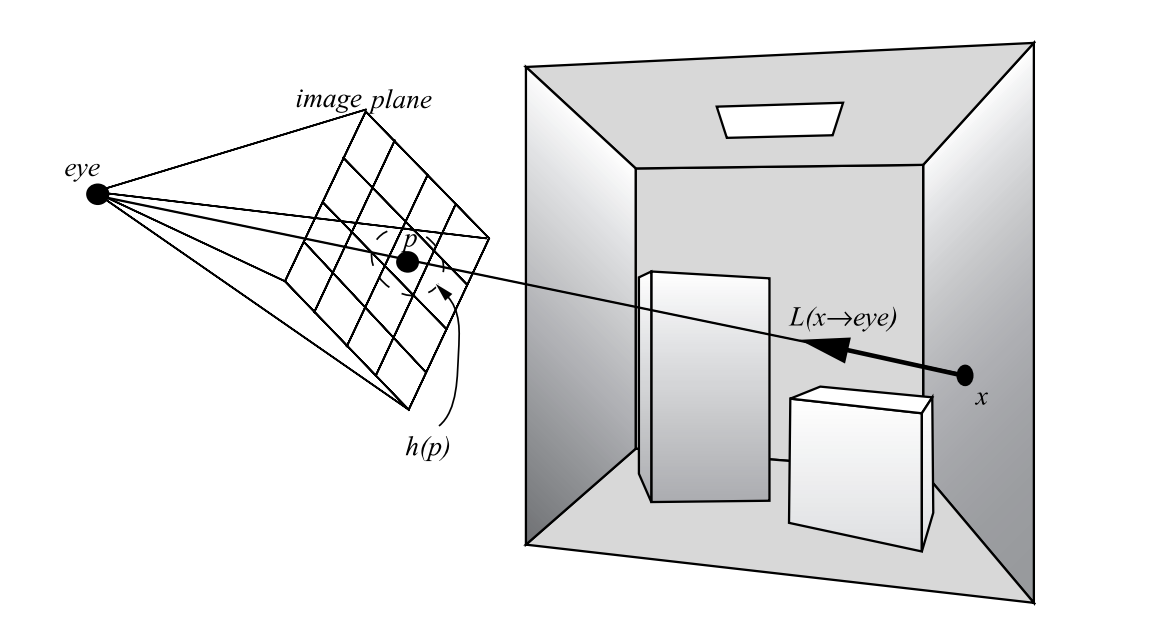
\includegraphics[scale=1]{obrazky-figures/ray_tracing_plane.png}
	\boldcaption[\textbf{Vrhání paprsku do scény.}]{ Počátkem paprsku je \textit{eye}, nebo-li umístění kamery. Paprsek dále prochází \textit{image plane}, což je rovina odpovídající výslednému vykreslenému obrázku. Převzato z Advanced global illumination \cite{advanced_global}.}
	\label{fig:scene_ray}
\end{figure}


Jak napovídá již samotný název -- ray tracing používá paprsky k~výpočtu barvy výsledného obrázku. Paprsek je polopřímka a je tedy definován počátečním bodem $\Vec{o}$ (origin) a směrem $\Vec{d}$ (direction). Nutnou funkcí pro funkčnost tohoto algoritmu je výpočet průsečíku paprsku s~primitivy, pomocí kterých je scéna vytvořena. Možnosti výpočtu průsečíku paprsku s~voxelem jsou uvedeny v~sekci \ref{sec:voxel_render}. Jednoduchý ray tracing je popsán algoritmem \ref{alg:rt_1}. Takto zjednodušená implementace je v praxi samozřejmě velice neefektivní a pro běžně používané scény je nutné použít akcelerační struktury pro urychlení hledání průsečíku jak uvádí kniha \cite{accelerated_rt}. Pro realistické zobrazování jsou kromě primárních paprsků generovány i paprsky sekundární. Tyto paprsky jsou použity například pro odrazy, refrakci a stíny.

Ve své standardní formě ray tracing neumožňuje generování měkkých stínů a spousty dalších sekundárních efektů.  Pro dosažení kýženého efektu lze využít například \textbf{Monte carlo ray tracing} (stochaistic ray tracing nebo distributed ray tracing) \cite{distributed_rt}. Namísto jediného paprsku pro výpočet stínů, odrazů a refrakcí je využito paprsků více a výsledky jejich výpočtu jsou následně průměrovány. Metoda umožňuje vytvoření mnoha dalších efektů, mezi které patří například hloubka pole, rozmazání pohybu a další.

\begin{center}
	\begin{czechalgorithm}[H] \label{alg:rt_1}
		ray = build\_ray(camera.position, image\_plane)\\
		min\_distance = MAX\\
		hit\_primitive = false\\
		\ForEach{\text{primitive in scene}} {
			(intersected, distance) = intersect(ray, primitive)\\
			\uIf{intersected \And distance < min\_distance}{
				hit\_primitive = primitive\\
				min\_distance = distance
			}
		}
		\caption{Ray tracing}
	\end{czechalgorithm}
\end{center}

\subsubsection{Ray marching}
Další metoda, kterou by bylo vhodné zmínit, je taktéž algoritmus ray marching (sphere tracing). Namísto přímého výpočtu průsečíku se scénou -- jak tomu je u~spousty ray tracing implementací -- prochází paprsek scénou postupně, dokud nedojde k~průsečíku.

\begin{figure}[H]
	\centering
	\captionsetup{justification=centering}
	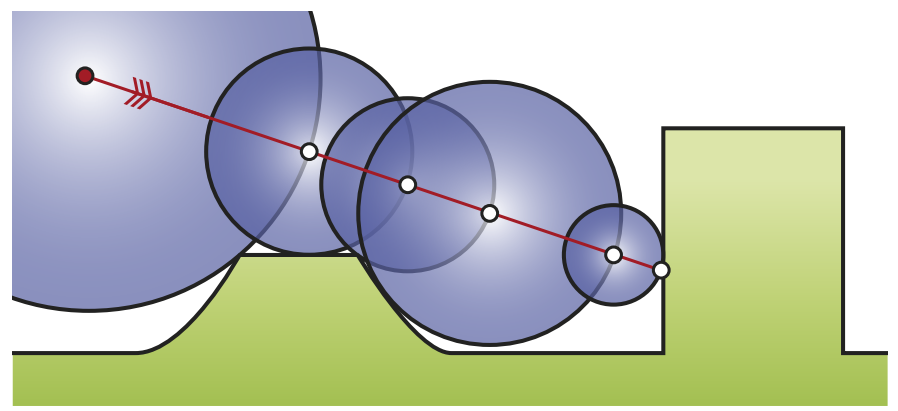
\includegraphics[scale=0.8]{obrazky-figures/ray_marching.png}
	\boldcaption[\textbf{Ray marching.}]{ Kružnice zobrazují vzdálenost současné pozice paprsku ke scéně, což odpovídá kroku paprsku v současné iteraci. Převzato z Enhanced Sphere Tracing \cite{Keinert2014EnhancedST}.}
	\label{fig:ray_marching}
\end{figure}

Článek \cite{sphere_tracing} popisuje algoritmus ray marching následovně: pro funkčnost algoritmu je podmínkou, aby existovala možnost vypočítat z~každého bodu ve scéně vzdálenost k~jejímu povrchu. Pro tento účel lze využít takzvaných signed distance functions (SDF). Každý paprsek, pro něž jeho generování probíhá stejně jako u~již zmíněného ray tracing, se iteruje napříč scénou, dokud do ní paprsek nenarazí, nepřekoná maximální počet iterací či maximální vykreslovací vzdálenost (algoritmus \ref{alg:ray_marching}).


\begin{center}
	\begin{czechalgorithm}[H] \label{alg:ray_marching}
		i = 0\\
		t = t\_min\\
		\While{t < t\_max \And i < MAX\_ITERATIONS}{\\
			distance\_to\_scene = dist\_func(ray)\\
			\uIf{distance\_to\_scene < \varepsilon}{\\
				\KwRet t\\
			}\\
			t += distance\_to\_scene\\
			i += 1\\
		}\\
		\KwRet t\_max\\
		\caption{Ray marching}
	\end{czechalgorithm}
\end{center}

Pro tento algoritmus existuje značné množství optimalizací \cite{Keinert2014EnhancedST}, jako je například "over-relaxation", kdy dochází k~záměrně většímu kroku a případnému návratu zpět. Dalším příkladem je namísto sledování paprsku použít kužel, což výrazně snižuje množství iterací algoritmu.


\subsubsection{Light field probes} \label{sec:light_field_probes}
Metoda globální iluminace využívající ray tracing byla představena v~publikaci \cite{light_field_probes}. Pracuje na předpokladu, že kontinuální světelné pole scény $\mathcal{L}(x, \omega)$, kde $x \in \mathcal{R}^3$ je bod v~prostoru a $\omega \in S$ je odchozí směr, reprezentuje distribuci osvětlení ve scéně pro všechny body a směry ve scéně. Light field probes reprezentuje tuto distribuci pomocí diskrétního vyobrazení.

Prostor ve scéně je rozdělen pomocí pravidelné mřížky. Do každé diskrétní pozice $x'$ je umístěna instance jedné sondy (probe), která mapuje směry $\omega$ kolem $x'$ na: intenzitu osvětlení $\mathcal{L}(x, \omega)$, normály $\vec{n}_x$ v~bodech $x''$ nejblíže bodu $x'$ a hloubkovou mapu mezi $x'$ a body $x''$. K výpočtu těchto hodnot dochází při přípravě scény.

\begin{figure}[H]
	\centering
	\captionsetup{justification=centering}
	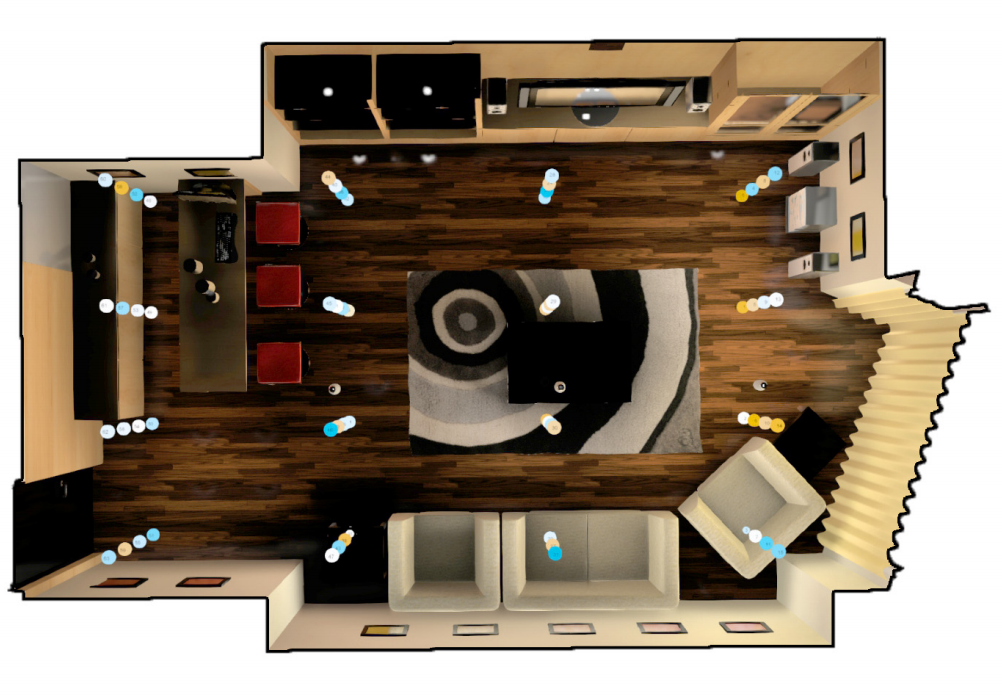
\includegraphics[scale=0.25]{obrazky-figures/light_field_probes.png}
	\boldcaption[\textbf{Umístění sond ve scéně.}]{ Pro obecné případy jsou sondy rozmístěny ve scéně rovnoměrně ve formě mřížky. Převzato z Real-Time Global Illumination Using Precomputed Light Field Probes \cite{light_field_probes}.}
	\label{fig:probes_in_scene}
\end{figure}

Algoritmus vykreslování postupuje napříč připravenými sondami. Při průchodu paprskem dochází k~výběru sondy, trasování uvnitř ní a následně je tento proces opakován napříč scénou, dokud nedojde k~jistému protnutí nebo minutí geometrie scény.

\subsection{Radiozita}
Metody radiozity byly vyvinuty již v~padesátých letech minulého století pro simulaci tepelného přenosu. Později byla popsána varianta pro vykreslování v~článku \cite{radiosity}. Metoda je založena na jednoduchém principu -- vzhledem k~tomu, že každý povrch ve scéně může odrážet světlo, je možné tento povrch považovat za zdroj světla. Radiozita povrchu je dána rovnicí \ref{eq:voxel_coords},


\begin{equation} \label{eq:voxel_coords}
	\begin{gathered}
		B_i = E_i + \rho_i \sum^N_{j = 1}B_jF_{ij} \text{ pro } i = 1 \text{ do } N
	\end{gathered}
\end{equation}

kde $B$ je celkové množství energie vyzařované z~povrchu, $E$ je množství energie vyzařované z~povrchu bez vlivu okolí, $\rho$ je faktor reflexivity, $F$ je faktor určující jaká část energie dorazila na povrch a $N$ je počet povrchů ve scéně.

Z~autorova průzkumu vyplývá, že je radiozita primárně používána pro předvýpočet globální iluminace v~některých scénách a dále není opakovaně počítána. Důvodem je nejspíše poměrně značná náročnost algoritmu.

\subsection{Materiály}
Pro simulaci interakce světla s~povrchy je nutné mít tyto povrchy popsány určitými parametry. Použité parametry závisí na osvětlovacím modelu a také renderovacím algoritmu. Publikace \cite{materials} popisuje interakci světla s~povrchem rovnicí \ref{eq:surface_photon},

\begin{equation} \label{eq:surface_photon}
	\begin{gathered}
		(x, y, \theta, \phi, t, \lambda)_{in} \xrightarrow{} (x, y, \theta, \phi, t, \lambda)_{out}
	\end{gathered}
\end{equation}

kde levá strana reprezentuje foton interagující s~povrchem a pravá strana foton vycházející ven, $(x, y)$ je pozice na povrchu, $(\theta, \phi)$ je příchozí/odchozí směr, $t$ je čas interakce a $\lambda$ je vlnová délka. Pro zjednodušení lze z~rovnice odstranit čas, čímž je předpokládáno, že se vzhled povrchu s~časem nemění. Při diskretizaci vlnových délek je možné dosáhnout dalšího zjednodušení, produkující takzvanou BSSRDF (bidirectional scattering surface distribution function). Dalším zjednodušením může být ignorování podpovrchového rozptylu světla (subsurface scattering), jehož výsledkem je již známé BRDF (bidirectional reflectance distribution function) (rovnice \ref{eq:brdf}),

\begin{equation} \label{eq:brdf}
	\begin{gathered}
		f_r(\vec{c}, \hat{\omega_i} \xrightarrow{} \hat{\omega_0}) = \frac{dL_0(\vec{x}, \hat{\omega_0)}}{dE(\vec{x}, \hat{\omega_i}} \\
		= \frac{dL_0(\vec{x}, \hat{\omega_0)}}{L_i(\vec{x}, \hat{\omega_i)\cos \theta_i d\omega_i}}
	\end{gathered}
\end{equation}

kde $L_0$ je podíl intenzity světla vycházející z~povrchu na bodu $\vec{x}$ ve směru $\hat{\omega_0}$ a intenzity světla příchozího do bodu $\vec{x}$ ze směru $\hat{\omega_i}$.

\begin{figure}[H]
	\centering
	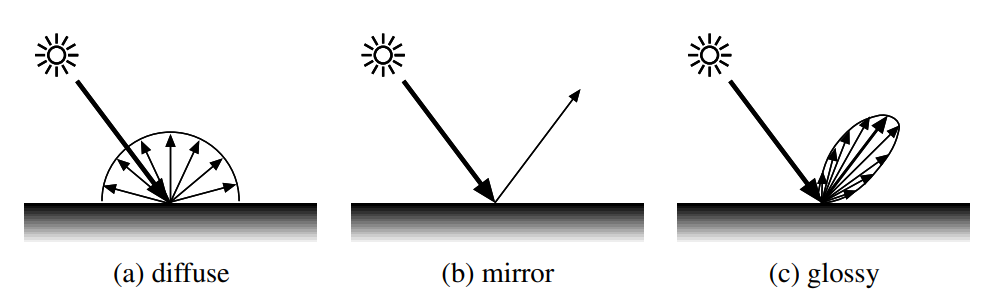
\includegraphics[scale=1]{obrazky-figures/reflection_types.png}
	\captionsetup{justification=centering}
	\boldcaption[\textbf{Typy odrazu světla.}]{ (a) difuzní, (b) zrcadlové, (c) lesklé. Převzato z Realistic Materials in Computer Graphics \cite{materials}.}
	\label{fig:refl_types}
\end{figure}

Dle knihy \cite{hunter_harold_1987} lze materiály dělit do několika základních kategorií podle typu interakce se světlem, přičemž tyto typy jsou uvedeny v tabulce \ref{tab:mats_distr}. Vizualizace některých možných odrazů světla znázorňuje obrázek \ref{fig:refl_types}.

\begin{table}[H]
	\centering
	\begin{tabular}{|l|l|}
		\hline
		materiál              & dominantní distribuce \\ \hline
		průhledný nemetalický & difuzní odraz         \\ \hline
		metalický             & zrcadlový odraz       \\ \hline
		průsvitný             & difuzní přenos        \\ \hline
		průhledný             & běžný přenos          \\ \hline
	\end{tabular}
	\captionsetup{justification=centering}
	\boldcaption[\textbf{Typy materiálů a jejich interakce se světlem.}]{ }
	\label{tab:mats_distr}
\end{table}


Dalším podstatným parametrem je tvar povrchu, který výrazně mění to, jak dochází k~odrazu světla. Vzhledem k~potenciální složitosti této vlastnosti se používají například následující metody:

\begin{itemize}
	\item Mapování normál (normal mapping)
	\item Parallax mapping
\end{itemize}

Příklady některých možných vlastností materiálů:

\begin{itemize}
	\item barva
	\item hrubost
	\item metalické
	\item mapa normál
	\item emisivita
	\item průhlednost
	\item odrazivost
	\item spousta dalších...
\end{itemize}


\subsection{Antialiasing}
Aliasing je nechtěný efekt při zpracování signálu, kdy dochází ke vzniku artefaktů při vzorkování. Při vykreslování se jedná především o~problém při vzorkování textur a artefakty na hranách objektu či přechodu mezi nimi (obrázek \ref{fig:aliasing}). Existuje množství metod pro odstranění tohoto efektu. Podle článku \cite{aa_survey} lze metody pro antialiasing dělit do následujících kategorií:

\begin{itemize}
	\item Full-Scene Anti-Aliasing (FSAA)
	\item Image Post-Processing Anti-Aliasing (IAA)
	\item Geometric Anti-Aliasing (GAA)
\end{itemize}

Každá z~těchto kategorií má mírně odlišný přístup k~problému aliasingu s~různými limitacemi.

\begin{figure}[H]
	\centering
	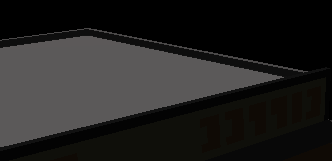
\includegraphics[scale=2]{obrazky-figures/aliasing.png}
	\captionsetup{justification=centering}
	\boldcaption[\textbf{Aliasing.}]{ Ukázka aliasingu vznikajícího kvůli nedostatečnému rozlišení výsledného obrázku.}
	\label{fig:aliasing}
\end{figure}

Příkladem FSAA je \textbf{Super Sampling Anti-Aliasing (SSAA)}, kde je počet pixelů pro renderování navýšen oproti cílové velikosti renderovaného obrázku. Při dokončení jsou přilehlé pixely a jejich barva/hloubka zprůměrovány. Tato metoda dosahuje výborných výsledků, ale je velmi výpočetně náročná. Optimalizovanou alternativou je \textbf{Multisample Anti-Aliasing (MSAA)}. Jedná se o~metodu fungující na stejném principu, ale namísto navýšení rozlišení celého renderovaného snímku dochází k~výběru oblastí, u~kterých je velká pravděpodobnost vzniku aliasingu a super sampling probíhá pouze v~těchto oblastech.

Z~rodiny IAA uveďme \textbf{Morphological Anti-Aliasing (MLAA)}. Tato metoda si dává za cíl minimalizovat aliasing z~okrajů a siluet. Algoritmus detekuje podezřelé oblasti podle rozdílu sousedních pixelů a používá rozmazání s~okolím. Detekce aliasingu může být i složitější, jako například vyhledávání specifických tvarů.


Vybraný zástupce GAA je \textbf{Geometric PostProcessing AA (GPAA)}. Při renderování obrazu dochází k~ukládání informací o~geometrii scény do separátního bufferu. Podle vzdálenosti sousedních pixelů ve finálním kroku dochází k~rozhodnutí, zda je nutné provádět anti-aliasing. Pokud ano, jsou vypočteny hodnoty okolních pixelů a dochází k~rozmazání.

\begin{figure}[H]
	\centering
	
\includegraphics[scale=3]{obrazky-figures/ssaa_diff.png}
	\captionsetup{justification=centering}
	\boldcaption[\textbf{Rozdíl kvality po použití SSAA.}]{ Levá polovina obrázku obsahuje snímek, ve kterém není využit anti-aliasing. V pravé části bylo využito SSAA.}
	\label{fig:aliasing_ssaa}
\end{figure}




\section{Voxel} \label{voxels}
Jak uvádí kniha \cite{gfx_principles_practice}, voxel, neboli \textbf{vo}lume \textbf{el}ement, reprezentuje hodnotu na pravidelné mřížce ve 3D prostoru (obrázek \ref{fig:3d_grid}). Díky tomu, že je prostor rozdělen mřížkou pravidelně, lze voxel definovat pomocí tří-složkového vektoru (rovnice \ref{eq:voxel_coords}). Pro účely vykreslování jsou voxelům přiřazovány další vlastnosti, jako například barva nebo materiál.

\begin{equation} \label{eq:voxel_coords}
	\begin{gathered}
		\vec{pozice_{voxel}} \in \mathbb{Z}_3
	\end{gathered}
\end{equation}

\begin{figure}[H]
	\centering
	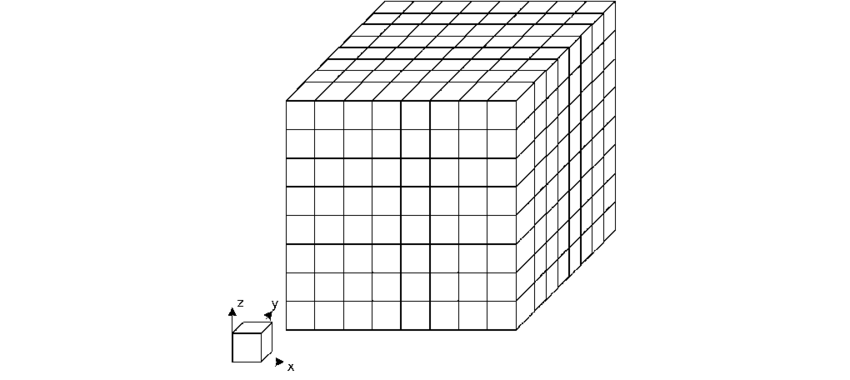
\includegraphics[scale=0.5]{obrazky-figures/3d_grid.png}
	\captionsetup{justification=centering}
	\boldcaption[\textbf{3D mřížka.}]{Převzato z Applied Mathematics and Computation \cite{3d_grid_image}.}
	\label{fig:3d_grid}
\end{figure}

Voxely jsou často využívány v~medicíně \cite{medical_vox}, například pro výstupy magnetické resonance (obrázek \ref{fig:mri_vox}).

\begin{figure}[H]
	\centering
	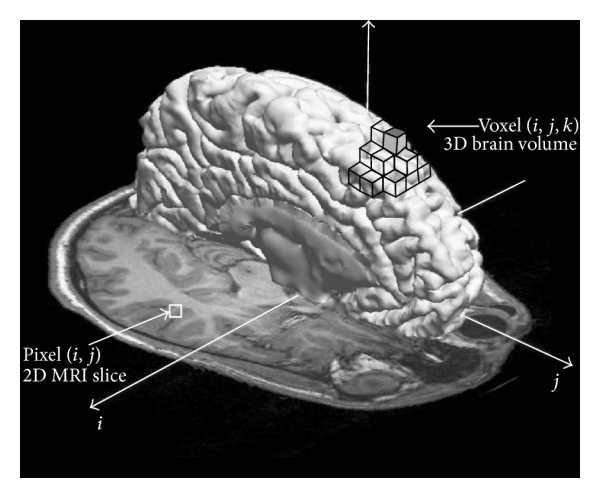
\includegraphics[scale=1]{obrazky-figures/voxel_mri.png}
	\captionsetup{justification=centering}
	\boldcaption[\textbf{Zobrazení výsledku magnetické resonance pomocí voxelů.}]{Převzato z Computational and Mathematical Methods in Medicine \cite{mri}.}
	\label{fig:mri_vox}
\end{figure}

Dalším častým využitím je modelování terénu, kde voxely přináší možnost reprezentovat převisy, čímž je terén značně realističtější než je tomu při aplikaci často používaných výškových map. Pravděpodobně nejznámější software používající voxely pro terén je \textbf{Minecraft} (obrázek \ref{fig:minecraft}). Za zmínku stojí také hra \textbf{Teardown} (2020)\footnote{\url{https://www.teardowngame.com/}}, kde je celý herní svět vytvořen pomocí voxelů a umožňuje téměř neomezenou destrukci.

\begin{figure}[H]
	\centering
	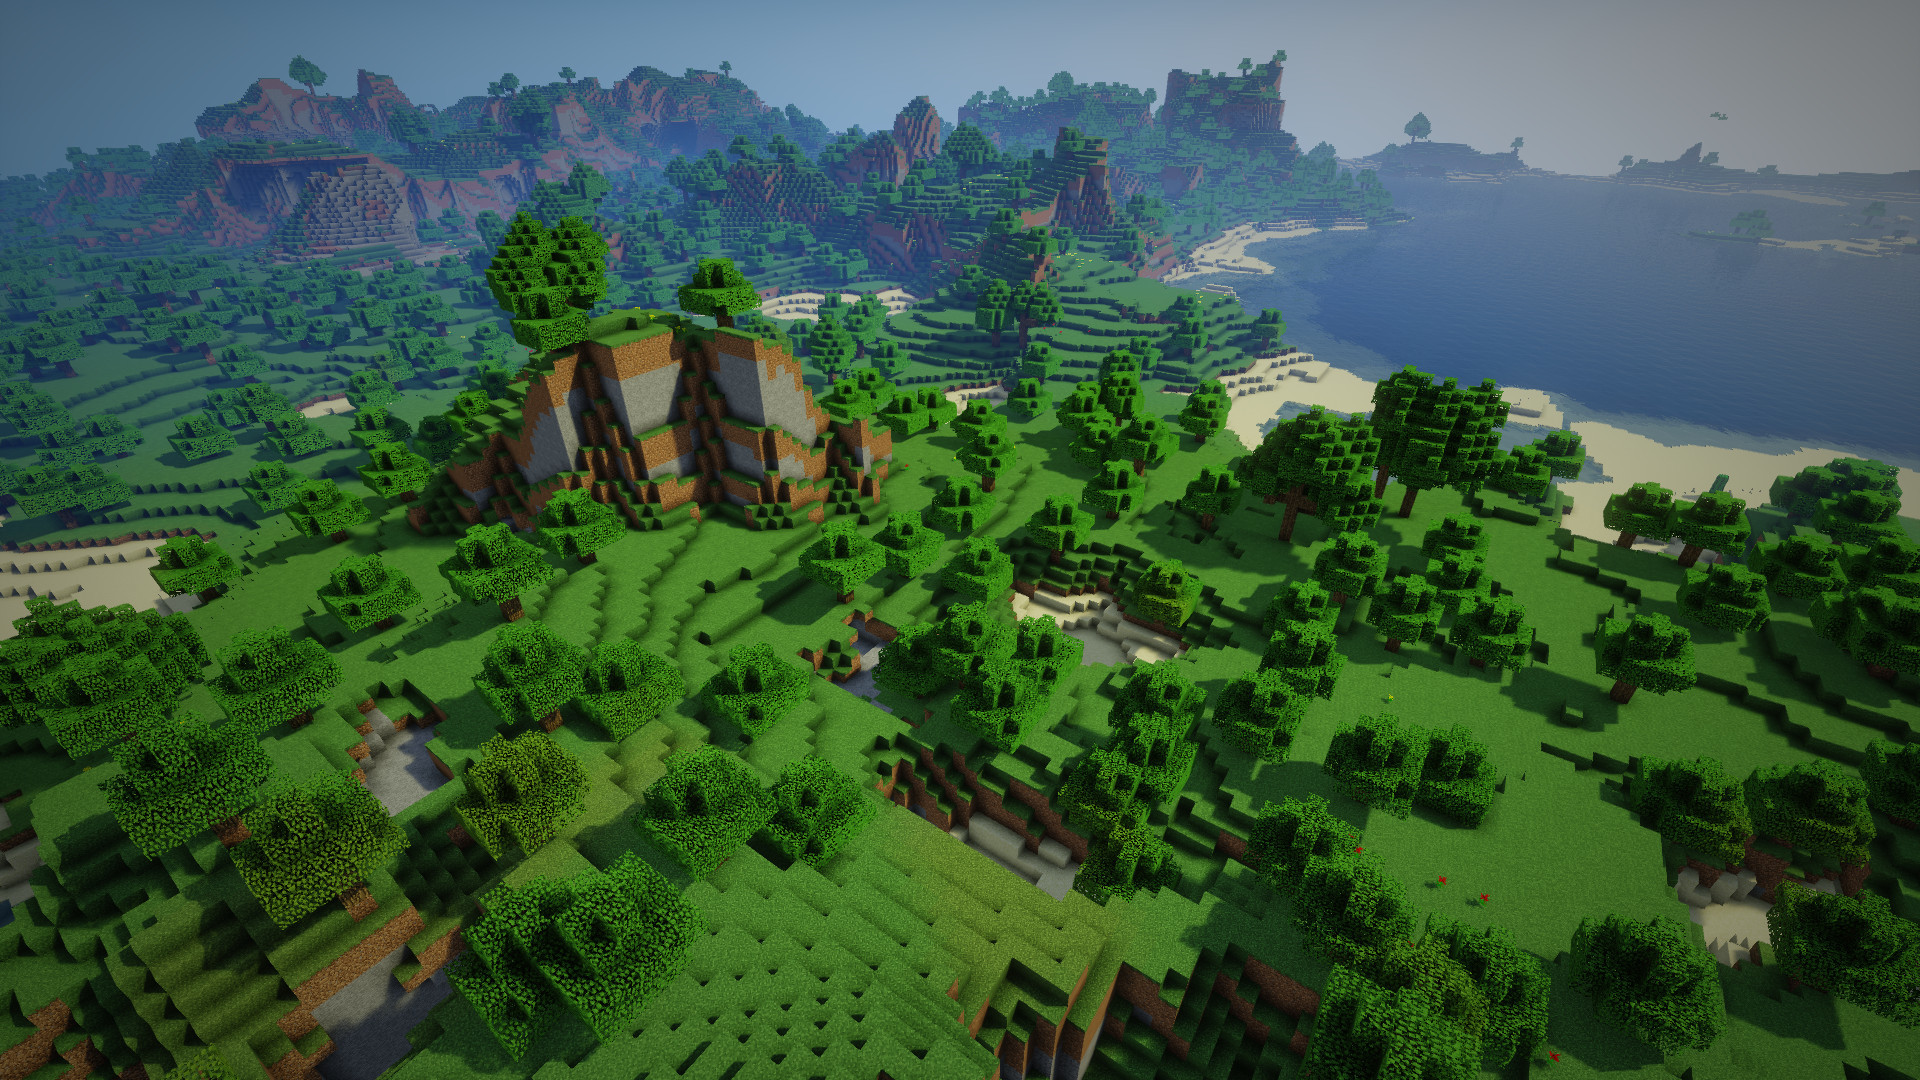
\includegraphics[scale=0.13]{obrazky-figures/minecraft.jpg}
	\captionsetup{justification=centering}
	\boldcaption[\textbf{Minecraft.}]{ Převzato z \url{https://forums-cdn.spongepowered.org/uploads/default/original/2X/8/83abd20efc6cf5104c2f8c5459808bcd1addef7a.jpg}.}
	\label{fig:minecraft}
\end{figure}

\subsection{Vykreslování voxelových modelů}\label{sec:voxel_render}
Níže jsou popsány základní metody vykreslování voxelových modelů. Jedná se jen o~základní příklady. Ve skutečnosti existuje mnohem více metod, než by bylo rozumné zde popisovat.

\subsubsection{Rasterizace}
Pro vykreslování voxelových scén pomocí rasterizace je nutné ji převést na trojúhelníkovou reprezentaci. Toho se dá dosáhnout několika způsoby.

\paragraph{Instanced rendering} je velice primitivní metoda. Pro každý voxel, který je reprezentován přímo svojí pozicí a případně dalšími parametry (barva...), je vykreslena krychle o~předem určené délce hran. Před samotným vykreslováním musí docházet k~odstranění takových voxelů, které nejsou viditelné. Pokud by byl tento krok vynechán, bylo by vykreslování velice náročné. \cite{nousiainen_2019}

\begin{center}
	\begin{czechalgorithm}[H] \label{alg:instanced_cube}
		voxel\_array = cull\_voxels(all\_voxels)\\
		\ForEach{\text{voxel in voxel\_array}} {\\
			render\_cube(voxel.position)\\
		}\\
		\caption{Instancované vykreslování}
	\end{czechalgorithm}
\end{center}

\paragraph{Marching cubes \cite{marching_cubes}} je příkladem algoritmu pro extrakci povrchu z~voxelových dat. Původně představen pro vizualizaci dat v~medicínském odvětví, je současně využíván například pro vizualizaci terénu \cite{nguyen_2008}. Pro každou oblast v~mřížce prostoru je zjištěno, který z~rohů voxelu se nachází uvnitř či vně tělesa. Na základně toho je vypočten tvar a pozice generovaných trojúhelníků. V~některých úpravách algoritmu je možné značně snížit počet vygenerovaných trojúhelníků a snížení redundantnosti dat. Po vygenerování často dochází k~minimalizaci počtu trojúhelníku. Algoritmus \ref{alg:marching_cubes} obsahuje zjednodušenou verzi této metody.

\begin{center}
	\begin{czechalgorithm}[H] \label{alg:marching_cubes}
		\ForEach{voxel in area} {\\
			case = calculate\_case(voxel)\\
			triangles = generate\_triangles(voxel.position, case)\\
			result.add(triangles)\\
		}\\
		\caption{Marching cubes}
	\end{czechalgorithm}
\end{center}

Existují další metody, jako například \textbf{marching tetrahedra}, ale tato práce rasterizačních metod nevyužívá a proto zde nebudou dále zmiňovány.

\subsubsection{Ray casting} \label{sec:voxel_intersection}
Při vykreslování pomocí paprsků lze problém rozdělit na dvě části. První z~nich je výpočet průsečíku s~voxelem a druhým je využití hierarchické struktury pro minimalizaci počtu navštívených voxelů. Hierarchické struktury jsou obsaženy v~samostatné sekci.

\paragraph{Průsečík paprsku s~voxelem} lze počítat mnoha způsoby. Primitivní přístup k~řešení tohoto problému je počítat průsečík s~každou rovinou, která reprezentuje voxel a následně vybrat ten nejbližší (algoritmus \ref{alg:ray_box_primitive}). Tohle řešení je ale poněkud náročné a využívá podmínky, což může podle článku \cite{gpu_branch} značně zpomalit výpočet.

\begin{center}
	\begin{czechalgorithm}[H] \label{alg:ray_box_primitive}
		corner_1 = voxel.position\\
		corner_2 = voxel.position + voxel\_length\\
		coeffs[0] = (corner_1.x - ray.origin.x) / ray.direction.x\\
		coeffs[1] = (corner_1.y - ray.origin.y) / ray.direction.y\\
		coeffs[2] = (corner_1.z - ray.origin.z) / ray.direction.z\\
		coeffs[3] = (corner_2.x - ray.origin.x) / ray.direction.x\\
		coeffs[4] = (corner_2.y - ray.origin.y) / ray.direction.y\\
		coeffs[5] = (corner_2.z - ray.origin.z) / ray.direction.z\\
		hit = false\\
		distance = \inf\\
		\ForEach{\text{coef in coefs}} {\\
			\uIf {coef >= 0} {\\
				hit = true\\
				hit\_point = ray.origin + ray.direction * coef;\\
				\uIf{is\_in\_box\_bounds(corner_1, hit\_point)}{\\
					distance = coef\\
				}
			}
		}
		\caption{Primitivní výpočet průsečíku s~voxelem}
	\end{czechalgorithm}
\end{center}

Vhodnější alternativu pro výpočet průsečíku paprsku s~voxelem lze najít v~publikaci \cite{efficient_box_intersect}. Tato metoda využívá dlaždic (slabs), kdy je voxel považován za průsečík tří z~nich. Na obrázku \ref{fig:slabs} je vizualizace výpočtu. Algoritmus pro 2D je popsán v~rovnici \ref{eq:slabs}.


\begin{equation} \label{eq:slabs}
	\begin{gathered}
		x_{min} = p_x + t_{xmin} d_x\\
		t_{xmin} = \frac{(x_{min} - p_x)}{d_x}\\
		\\
		y_{min} = p_y + t_{ymin} d_y\\
		t_{ymin} = \frac{(y_{min} - p_y)}{d_y}\\
		\\
		t_{xenter} = \min(t_{xmin}, t_{xmax})\\
		t_{xexit} = \max(t_{xmin}, t_{xmax})\\
		\\
		t_{yenter} = \min(t_{ymin}, t_{ymax})\\
		t_{yexit} = \max(t_{ymin}, t_{ymax})\\
		\\
		t_{exter} = \max(t_{xenter}, t_{yenter})\\
		t_{exit} = \min(t_{xexit}, t_{yexit})\\
	\end{gathered}
\end{equation}

\begin{figure}[H]
	\centering
	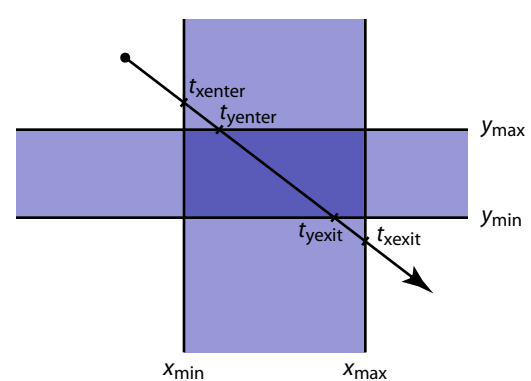
\includegraphics[scale=1.3]{obrazky-figures/slab_intersect.png}
	\captionsetup{justification=centering}
	\boldcaption[\textbf{Průsečík s obdélníkem metodou dlaždic.}]{ Vizualizace výpočtu ve 2D. Ve 3D se výpočet provádí velice podobně. Převzato z Ray Tracing: intersection and shading \cite{Cunha13}.}
	\label{fig:slabs}
\end{figure}


\subsection{Používané formáty} \label{sec:format}
Pro ukládání voxelových scén existuje poměrně velké množství formátů. Bohužel však neexistuje žádný standardizovaný formát, i když nějaké pokusy o standardizaci se již objevily (například VolDat\footnote{\url{http://www.volumesoffun.com/voldat-format/}}). Následující část textu popisuje vybrané formáty.

\paragraph{Vox} formát byl vytvořen pro aplikaci MagicaVoxel\footnote{\url{http://ephtracy.github.io/}}, což je modelovací software pro voxelové scény. Jedná se o~binární formát, kde jsou barvy zakódovány pomocí palety. Formát podporuje také různé typy materiálů, ač s malým množstvím parametrů. Scéna je složena z částí (modelů), které mají maximální velikost 256x256x256 voxelů -- při načítání je tedy nutné rozhodnout, zda je celý soubor jedním modelem, nebo je rozdělen na chunky. Specifikace formátu jsou v~\cite{vox_format}.

\begin{figure}[H]
	\centering
	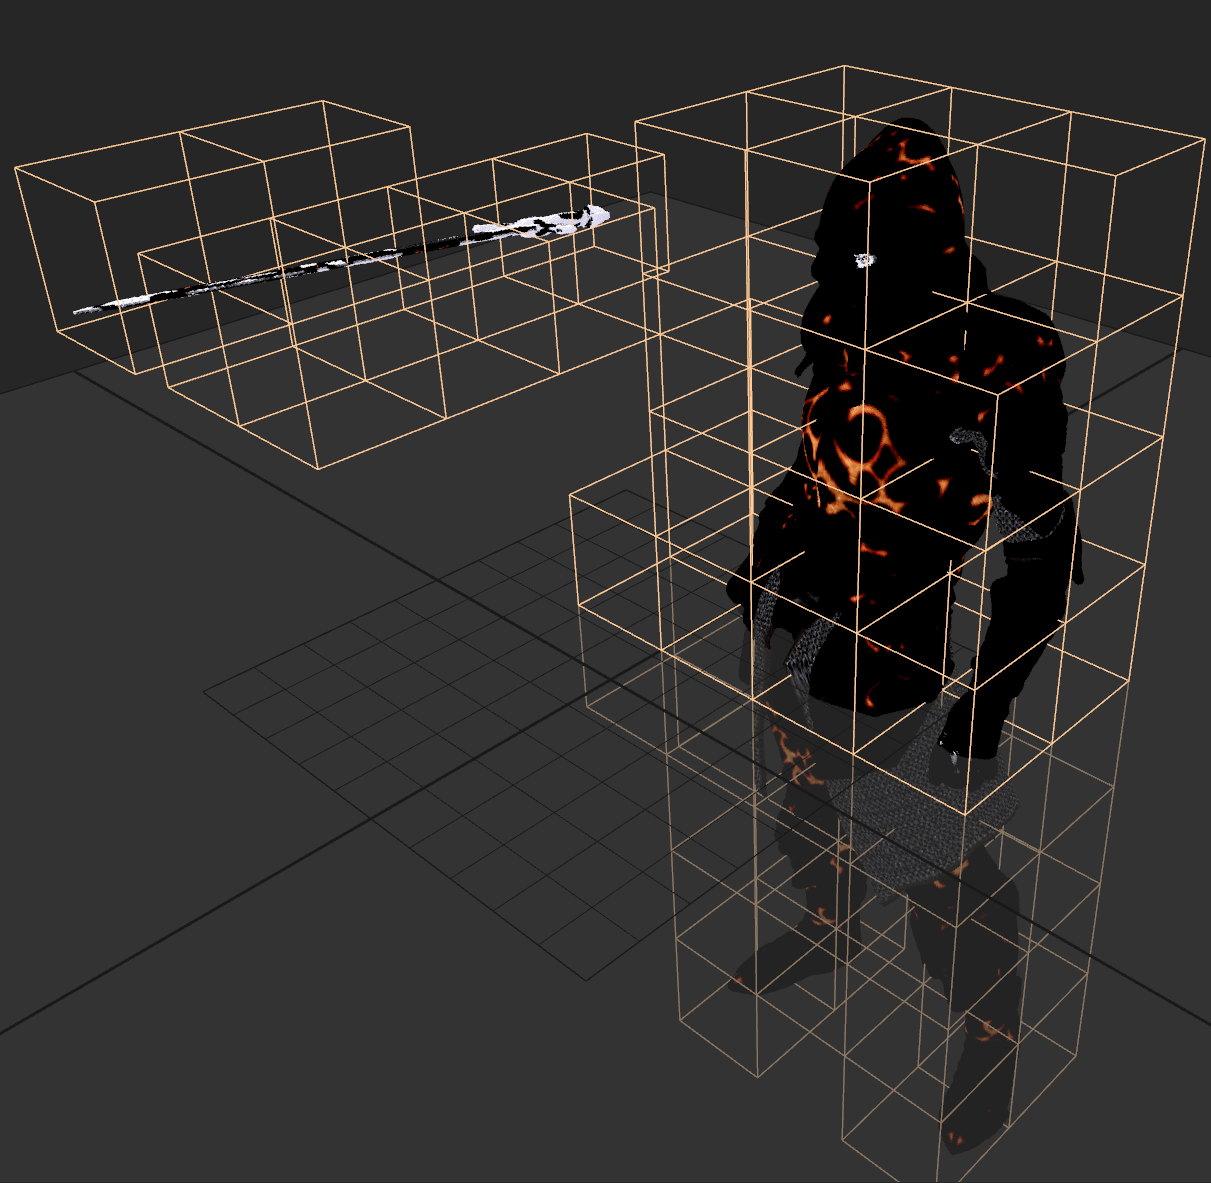
\includegraphics[scale=0.5]{images/magica_voxel_vox.png}
	\captionsetup{justification=centering}
	\boldcaption[\textbf{VOX model rozdělený na chunky.}]{ Dělba modelů na chunky, zobrazeno pomocí MagicaVoxel.}
	\label{fig:magica_vox}
\end{figure}

\paragraph{SVX} (Simple Voxels) je archivový formát. Archiv obsahuje soubor manifest.xml, který popisuje velikost mřížky, velikost voxelů, paletu materiálů a další metadata. Samotné voxely jsou popsány pomocí obrázků v~jednokanálovém formátu PNG, přičemž každý pixel slouží jako odkaz do palety modelů. Tento formát je používán především pro 3D tisk. Specifikaci formátu lze nalézt na \cite{svx_format_2014}.

Existuje spousta dalších formátů, značné množství pro 3D tisk, ale také pro využití v~medicíně, jak již bylo zmíněno dříve. Dle autorova průzkumu je nejčastějším přístupem při volbě formátu pro vykreslovací engine vytvoření vlastního formátu.

\paragraph{VolDat} byl vytvořen jako pokus o jistou formu standardizace voxelových formátů. Tento formát byl popsán v \cite{williams_2013}. Scéna je rozdělena na 2D části (průřezy napříč osou Y) a každý tento průřez je uložen v obrázku. Pixely obrázku reprezentují jednotlivé voxely, jejich hodnota vyjadřuje barvu a také odkaz do separátního textového souboru, kde jsou uloženy doplňující data, jako například informace o materiálech. 


\section{Hierarchické struktury}
Jak již bylo zmíněn -- pro efektivní práci s~velkým množstvím voxelů je potřeba využít akceleračních struktur. V~této sekci je obsažen popis některých struktur, které se dají pro voxely použít.

\subsection{Mřížka}
Mřížka, nebo také grid, je poměrně jednoduchá struktura pro dělbu prostoru. Na nejnižší úrovni může mřížka odpovídat té, pomocí které dělí prostor samotné voxely. V~takovém případě by však nedošlo k~žádnému zrychlení. Pro akceleraci je prostor obsahující voxely rozdělen do několika částí (tzv. chunks). V~těchto oblastech jsou voxely sdružovány a při hledání požadované položky je možné nejdříve vybrat správný chunk a teprve následně vyhledávat v~omezené množině voxelů. Samotná struktura má minimální paměťové nároky, ale nepřináší velké zrychlení, alespoň ve srovnání s~ostatními metodami. Jednoduchá trojrozměrná mřížka je na obrázku \ref{fig:3d_grid}.

\subsection{Hierarchie obalových těles} \label{sec:BVH}
Obalové těleso (bounding volume) je jednoduchý geometrický objekt, který obaluje jeden či více objektů s větší komplexitou \cite{ericson_2005}. Důležitým faktorem pro vhodnost tělesa k využití v hierarchii obalových těles (bounding volume hierarchies) pro ray tracing je náročnost výpočtu průsečíku s tělesem. Jako příklad lze uvést kouli (rovnice \ref{eq:sphere_ray_intersection}), osově zarovnaný obdélník (axis aligned box) nebo konvexní obálku. 

\begin{equation} \label{eq:sphere_ray_intersection}
	\begin{gathered}
	    R(t) = \textbf{o} + t\textbf{d}  \\
	    
	    (P + t\textbf{d} - C) (P + t\textbf{d} - C) = r^2
	    
	\end{gathered}
\end{equation}

\begin{eqexpl}[60mm]
\item{$R$} paprsek
\item{$\textbf{o}$} počátek paprsku
\item{$t$} vzdálenost průsečíku
\item{$\textbf{d}$} směr paprsku
\item{$C$} střed koule
\item{$r$} poloměr koule
\end{eqexpl}

Samotná hierarchie těchto těles je tvořena jako stromová struktura, kde každý nelistový uzel obsahuje zpravidla 2 potomky. Obalové těleso reprezentující nelistové uzly je vytvořeno tak, aby ohraničovalo pouze prostor nutný k obsažení jeho potomků.

\begin{figure}[H]
	\centering
	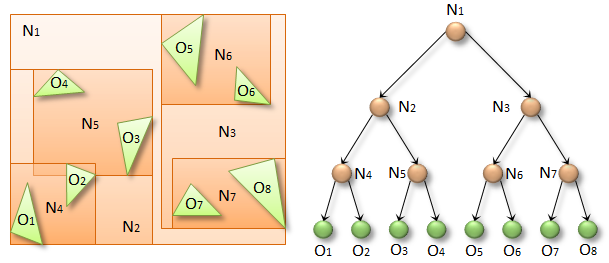
\includegraphics[scale=0.5]{images/fig03-bvh.png}
	\captionsetup{justification=centering}
	\boldcaption[\textbf{2D hierarchie obalových těles.}]{ \textit{O} reprezentuje objekty ve scéně a \textit{N} uzly stromu. Převzato z \url{https://developer.nvidia.com/blog/thinking-parallel-part-ii-tree-traversal-gpu/}.}
	\label{fig:slabs}
\end{figure}

Díky snadnosti výpočtu průsečíků a možnosti netestovat průsečíky s nižšími úrovněmi stromu -- a tím i komplexními objekty -- může dojít k výraznému zrychlení výpočtu průsečíku se scénou. Algoritmus \ref{alg:bvh_traverse_naive} popisuje jednoduchý průchod binárním stromem za pomoci zásobníku.

\begin{center}
	\begin{czechalgorithm}[H] \label{alg:bvh_traverse_naive}
		current\_node = root\\
		stack = empty()\\
		exit = false\\
		\While{\text{!exit}} {\\
			\eIf{isInternalNode(current\_node)}{
			    \uIf{intersectNode(current\_node)}{
			        pushStack(stack, current\_node.first\_child)\\
			        current\_node = current\_node.second\_child\\
			    }
			}{
			    intersectLeaf(current\_node)\\
			    (current\_node, exit) = popStack(stack)\\
			}
		}\\
		\caption{Průchod BVH stromem pro ray tracing \cite{Vaidyanathan2019WideBT}}
	\end{czechalgorithm}
\end{center}



\subsection{Octree} \label{octree}
Octree, poprvé představen v~knize \cite{rensselaer1980octree}, je popsán jako hierarchický N-dimenzionální binární strom, jenž reprezentuje N-dimenzionální objekt. Pro účely tohoto textu je podstatná pouze jeho 3D varianta. Každý uzel stromu obsahuje 8 potomků na další úrovni. Tyto uzly reprezentují oblast v~prostoru. Pokud uzel kompletně popisuje oblast, kterou reprezentuje, jedná se o~list nebo koncový uzel. V~opačném případě musí obsahovat 8 potomků pro podoblasti. Při hledání objektů v~prostoru tedy lze procházet pouze velmi omezenými oblastmi a neplýtvat výpočetním výkonem.

\begin{figure}[H]
	\centering
	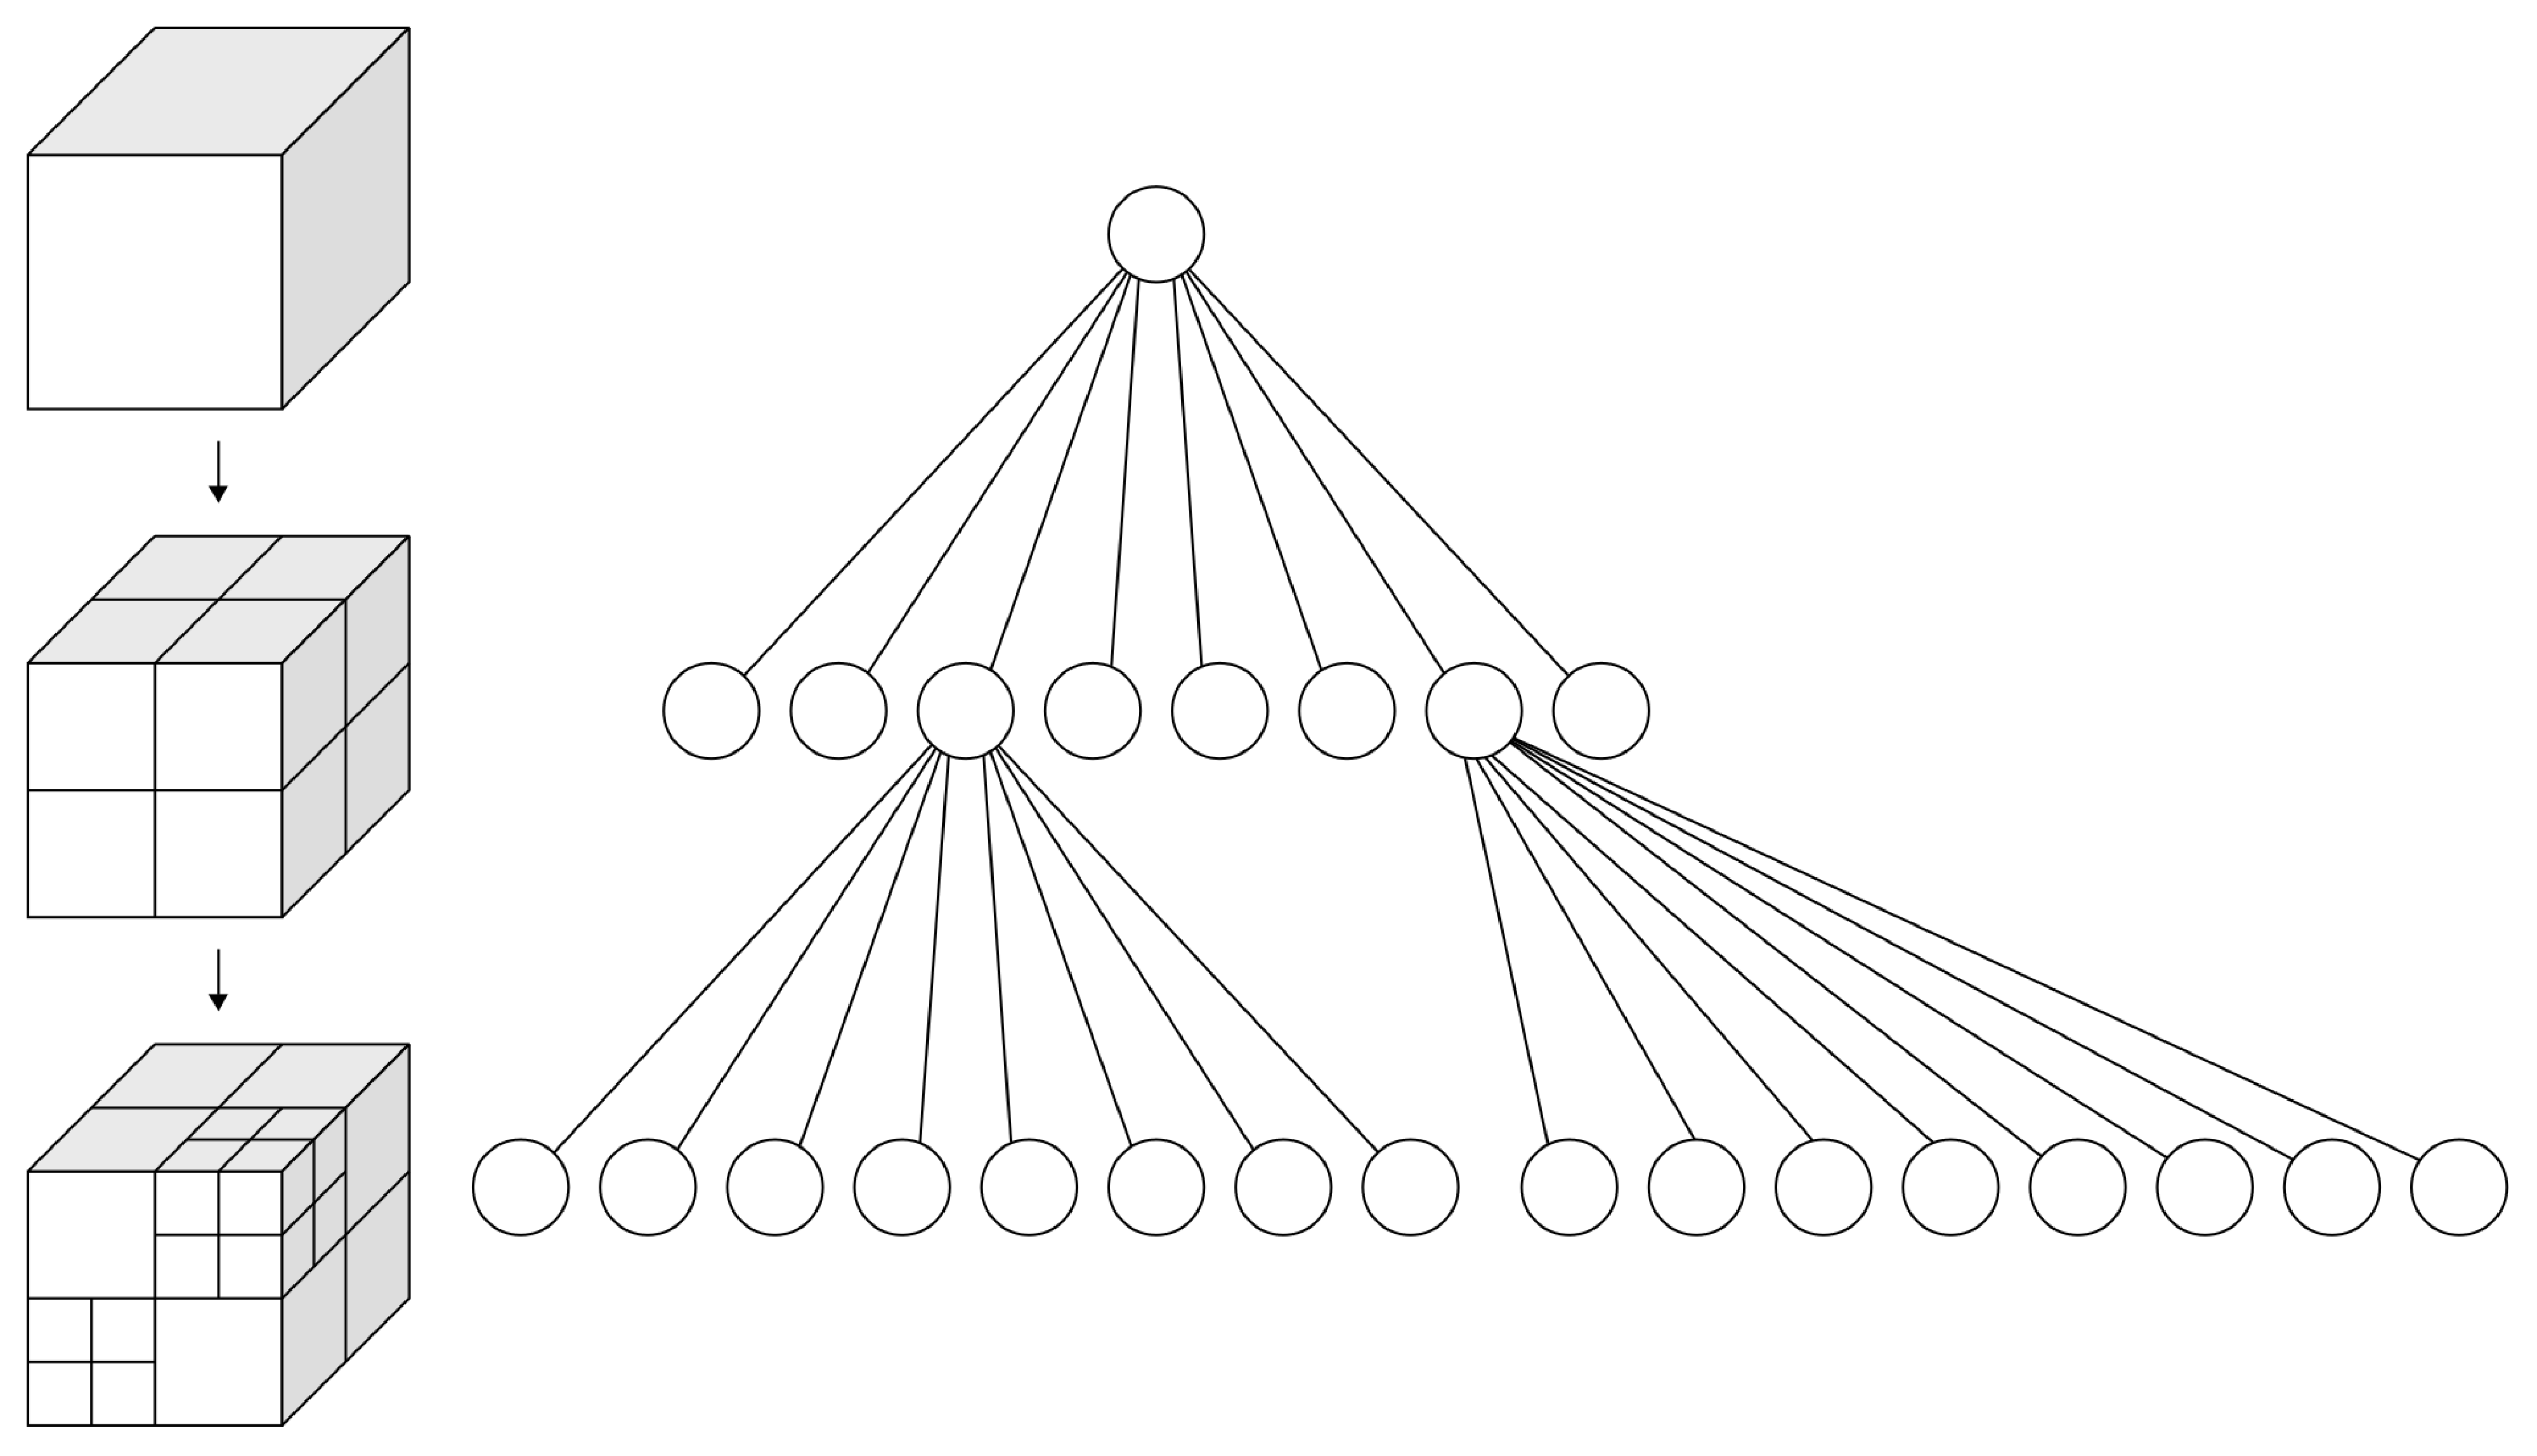
\includegraphics[scale=0.12]{obrazky-figures/Octree2.pdf}
	\captionsetup{justification=centering}
	\boldcaption[\textbf{Octree.}]{Převzato z \url{https://en.wikipedia.org/wiki/Octree}.}
	\label{fig:slabs}
\end{figure}


\subsubsection{Sparse voxel octree}\label{svo_alg}
Jedná se o renderovací metodu využívající ray casting/tracing pro vizualizaci voxelových scén. Důležitou částí generování octree pro tento algoritmus je minimalizace uzlů, které nejsou viditelné, či spojení stejných uzlů do jednoho bloku na vyšší úrovni \cite{Laine2011EfficientSV}. Výhodou je velmi snadná aplikace level of detail napříč stromem. Podle velikosti pixelu je možné zastavit průchod stromem před dosažením nejnižší úrovně a vypočítat výslednou barvu z~uzlu na vyšší úrovni. Algoritmus \ref{alg:svo} popisuje jednoduchou verzi algoritmu.

\begin{center}
	\begin{czechalgorithm}[H] \label{alg:svo}
		voxel = tree.get\_root()\\
		\While{not terminated}{\\
			(hit, t) = intersect\_cube(ray, voxel)\\
			\uIf{hit}{\\
				\uIf{is\_voxel\_small(voxel, pixel\_size) || is\_voxel\_leaf(voxel)}{\\
					\KwRet t\\
				}\\
				stack.push(voxel)\\
				voxel = select\_child(voxel)\\
				continue
			} \uElse {\\
				voxel = stack.pop()
			}\\
		}\\
		\KwRet false
		\caption{Sparse voxel octree ray casting}
	\end{czechalgorithm}
\end{center}

\section{Vulkan API}
Vulkan je API pro 3D grafiku a výpočty pomocí GPU \cite{vulkan_web}. Je produktem Khronos Group. Jedná se o nízkoúrovňové rozhraní s nízkou režií, které je zároveň multiplatformní. Produkty postavené na tomto API lze tedy spouštět na velkém množství různých systémů. Oproti OpenGL, které je jistým způsobem předchůdcem Vulkanu, je ve Vulkanu nutné nastavovat výrazně větší množství parametrů. Díky této vlastnosti má programátor podstatně větší kontrolu nad stavem grafické karty. Nevýhodou ovšem je značné zvýšení komplexity programu oproti jednodušším API. Některé výhody, které Vulkan poskytuje oproti jiným grafickým API:

\begin{itemize}
	\item Jednotné API jak pro mobilní zařízení, tak pro PC.
	\item Dostupnost na velkém množství operačních systému (podobně jako OpenGL).
	\item Nízký overhead.
	\item Pro shadery používá binární formát SPIR-V\footnote{\url{https://www.khronos.org/opengl/wiki/SPIR-V}}, díky čemuž mohou vývojáři distribuovat pouze binární formu shaderů.
	\item Sjednocení grafického (graphics pipeline) a výpočetního (compute shaders) API.
	\item Ray tracing pomocí rozšíření (tuto funkci podporuje i DirectX12).
\end{itemize}

Současnou verzí API je Vulkan 1.2.184\cite{vulkanspec}.

\chapter{Návrh řešení}
\label{navrh}
Následující část práce popisuje návrh aplikace pro realistické zobrazování voxelových scén. Kapitola je rozdělena na část popisu reprezentace voxelových dat a dále jejich vykreslování pomocí sparse voxel octree algoritmu.

\section{Reprezentace voxelových dat}\label{sec:voxel_representation}
Jak již bylo popsáno v~sekci \ref{voxels} -- voxely jsou reprezentovány svou pozicí a jejich materiální vlastnosti různými parametry. Logickým krokem je rozdělení těchto dvou vlastností. V~některých strukturách je lze kódovat implicitně a nemusíme tedy plýtvat paměťovým prostorem.

Pro implicitní zakódování pozice lze využít octree (sekce \ref{octree}). Nejnižší úroveň stromu reprezentuje samotné voxely a jediným nutným parametrem je počáteční pozice stromu a velikost prostoru, který obaluje. Samotný strom by mohl být vytvořen se statickým rozestupem rodičů a potomků, kde by se výpočet indexu následníka mohl řídit rovnicí:

\begin{equation} \label{eq:simple_octree_index}
	\begin{gathered}
		I_{child_j} = (i * 8) + j
	\end{gathered}
\end{equation}

kde $I_{child_j}$ je index $j$-tého potomka, $i$ je index současného uzlu. Při použití tohoto rozložení by ovšem musela být celá oblast uvnitř octree rozdělena na nejmenší bloky a docházelo by k~obrovskému plýtvání paměti.

\begin{figure}[H]
	\centering
	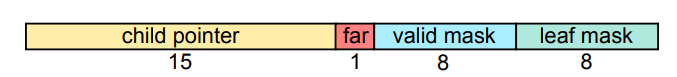
\includegraphics[scale=1.7]{obrazky-figures/octree_child_data.png}
	\captionsetup{justification=centering}
	\boldcaption[\textbf{Položka reprezentující uzel octree.}]{Převzato z \cite{Laine2011EfficientSV}.}
	\label{fig:octree_child}
\end{figure}

Úsporný způsob pro reprezentaci octree byl představen v článku \cite{Laine2011EfficientSV}. Metoda kóduje informace o~uzlu bitově na data o~velikosti 4 bytů. Vizualizace je na obrázku \ref{fig:octree_child}. Každý nelistový uzel je reprezentován svými daty a listové uzly jsou implicitně kódovány pomocí masek. \texttt{Child pointer} určuje pozici potomků uzlu pro daný uzel, přičemž je uložen jako rozdíl od pozice současného uzlu, čímž je možno ho reprezentovat menším rozsahem. Přepínač \texttt{far} určuje, zda \texttt{child pointer} odkazuje na pozice potomků, či na 32 bitový ukazatel na ně - při velkých stromech nemusí být 15 bitů dostačující. Tento pointer je uložen v~oddělené části bufferu. \texttt{Valid mask} je bitová maska o~velikosti 8 bitů, pokud je hodnota nastavena na 1, pak je ve stromu potomek na tomto indexu reprezentován. \texttt{Leaf mask} odpovídá funkci \texttt{valid mask}. Dává nám ovšem vědět, jestli je potomek na indexu terminálním uzlem. Pokud je tedy nastavena na 1, tak je vyhledávání ve stromu na této úrovni ukončeno.

Kromě informací o~obsazenosti prostoru je nutné ukládat i informace o~materiálu. První možností by bylo rozšířit záznamy ve stromu o~tato data, ale s~velkým množstvím parametrů by velikost stromu rapidně narostla. Proto by bylo vhodnější tato data ukládat separátně. Tyto informace také nejsou relevantní při procházení stromu a pokud by byla uložena ve struktuře, došlo by ke zhoršení prostorové lokality paměti. Vhodným řešením je za oblastí stromu vytvořit oblast s~ekvivalentní strukturou, kde jsou uloženy odkazy na materiálová data. Výpočet offsetu do struktury je triviální, jelikož je pozice dat na stejném indexu jako je index uzlu. Nalezené položky slouží k~vyhledávání specifického záznamu v~separátním bufferu. Výhodou tohoto přístupu je možnost snadno ukládat samostatné materiály pro vyšší úrovně stromu, což může být použito pro aplikaci level of detail.

\paragraph{Ukládání voxelových dat} Pro načítání modelů je využit formát VOX, který byl popsán v sekci \ref{sec:format}. Při načítání je ovšem nutné data transformovat do formátu octree popsaného výše, což může způsobit výrazné zpomalení aplikace. Namísto opakované transformace by bylo tedy vhodné data ukládat tak, aby docházelo pouze k načtení -- tím by došlo k výraznému zrychlení. Vzhledem k tomu, že je důležitá spíše rychlost a ne využití místa na disku, je dostačující serializovat strukturu popsanou výše přímo do binárního souboru. Zpravidla dojde k malému zvětšení oproti VOX, ale doba načítání se zkrátí na zlomek času.

\section{Vykreslování}\label{sec:rendering}
Následující sekce popisuje metody využité pro vykreslování scény v této práci -- jmenovitě ray marching pomocí sparse voxel octrees, light field probes a jejich modifikace pro nepřímé osvětlení.

\subsection{Sparse voxel octree}\label{sec:svo_design}
Pro rendering voxelové scény existuje několik možností, přičemž vhodným kandidátem je přístup sparse voxel octree (sekce \ref{svo_alg}). Při vržení paprsku dochází k~procházení stromu a vcházení pouze do podoblastí, které mohou obsahovat vyhledávaný voxel. Algoritmus je velice úsporný oproti primitivním metodám. Tato metoda je popsána v \cite{Laine2011EfficientSV}.

\begin{figure}[H]
	\centering
	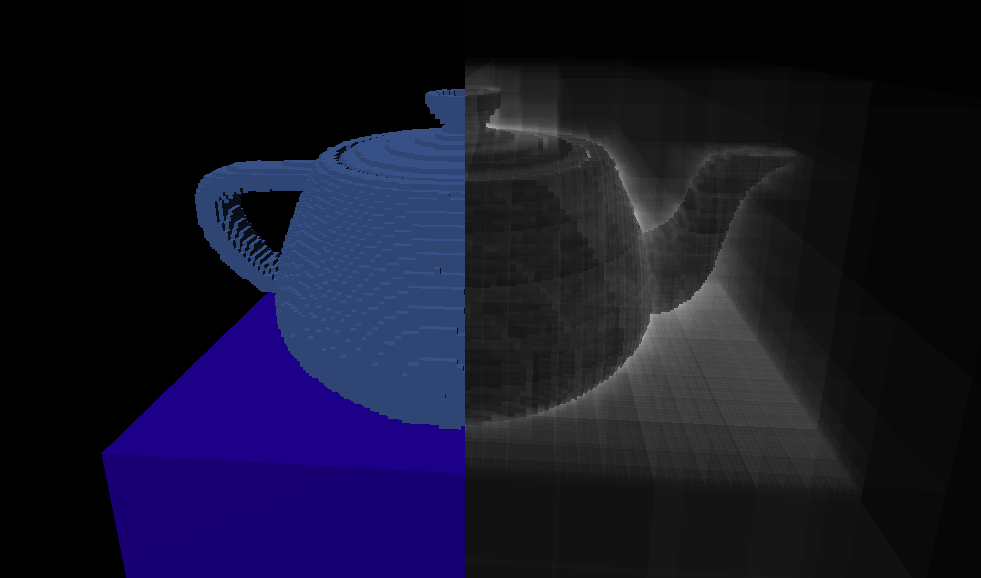
\includegraphics[scale=1]{obrazky-figures/color_iter_svo.png}
	\captionsetup{justification=centering}
	\boldcaption[\textbf{Render voxelizované "Utah teapot".}]{ Levá část vyobrazuje běžné vykreslení, pravá obsahuje počet iterací algoritmu v daném pixelu -- plně bílá barva je v tomto případě \textasciitilde{}128 iterací.}
	\label{fig:octree_child}
\end{figure}

Vzhledem ke způsobu uložení dat představenému v předešlé kapitole je v~rámci algoritmu nutné dopočítávat množství indexů uzlů na základě masek (\texttt{valid mask} a \texttt{leaf mask}). Jedná se ale zpravidla pouze o~operace sčítání či odčítáním, tedy operace s nízkou výpočetní náročností.

Pro výpočet průsečíku s~voxelem je vhodné využít optimálnější metody popsané v~sekci \ref{sec:voxel_intersection}. Důležitou součástí pro stínování je také získání normály povrchu. Vzhledem k~tomu, že cílem autora je zachovat "krychlovitý" tvar voxelů, je nalezení normály při využití slab metody pro nalezení průsečíku poměrně triviální.

\begin{figure}[H]
	\centering
	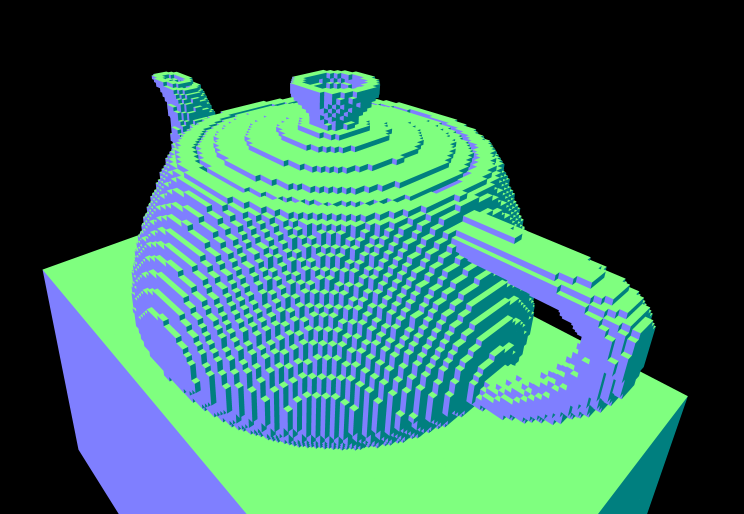
\includegraphics[scale=1]{obrazky-figures/normals_teapot.png}
	\captionsetup{justification=centering}
	\boldcaption[\textbf{Vizualizace normál pro model "Utah teapot".}]{ }
	\label{fig:octree_child}
\end{figure}

Pro usnadnění práce s modely a úsporu výpočetního výkonu při jejich transformaci má každý model svoji vlastní octree strukturu. Nutnost otestovat průsečíky se všemi těmito modely by byla velice náročná a proto je vhodné použít další akcelerační strukturu k urychlení nalezení průsečíku. Autor práce zvolil hierarchii obalových těles (sekce \ref{sec:BVH}) s využitím osově zarovnaných obdélníku. Každý listový uzel této hierarchie tedy obsahuje jeden octree, který definuje voxely modelu. 

\begin{figure}[H]
	\centering
	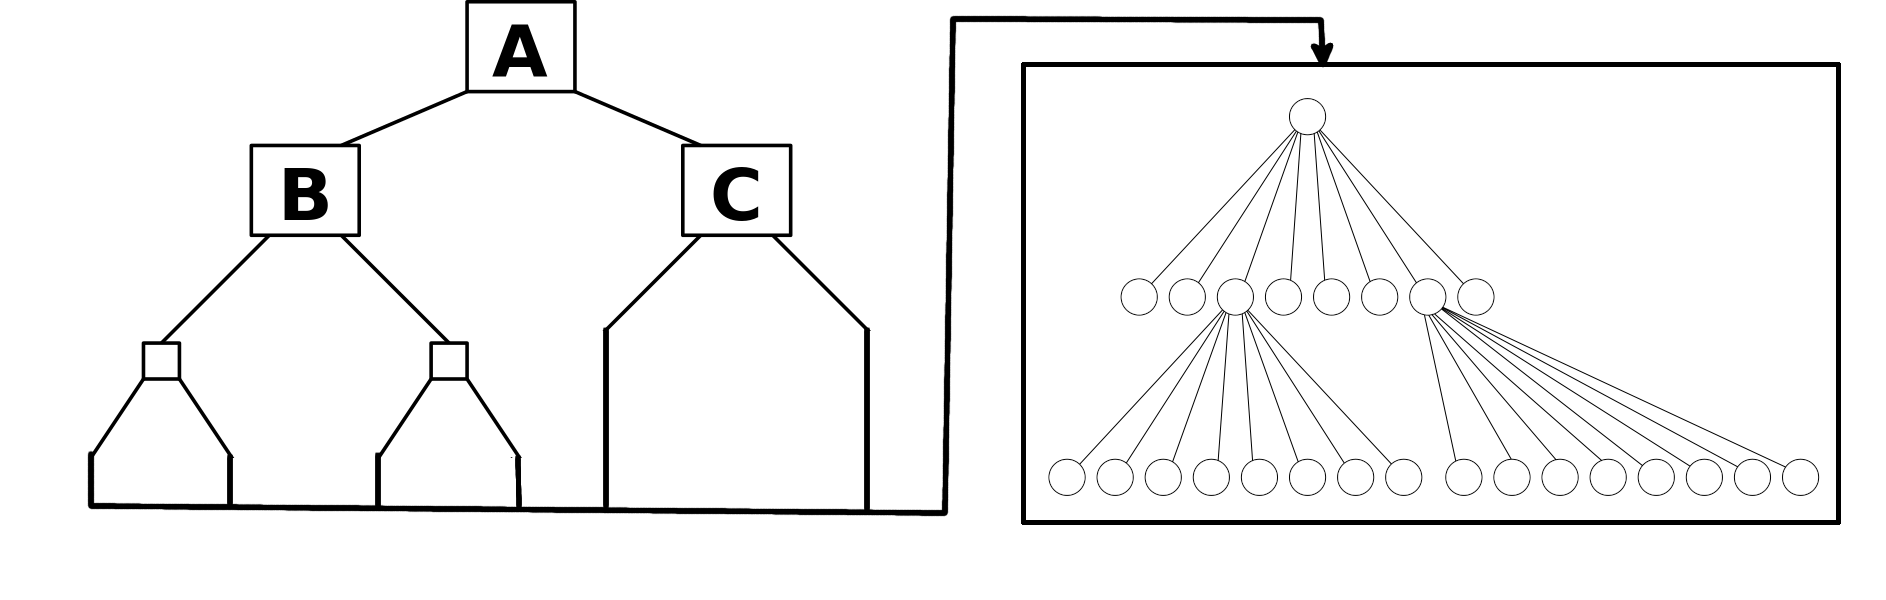
\includegraphics[scale=1]{images/bvh_octree.png}
	\captionsetup{justification=centering}
	\boldcaption[\textbf{Rozložení hierarchií scény.}]{ Levá část reprezentuje hierarchii obalových těles, kde se v každém listu nachází octree.}
	\label{fig:scene_bvh_repr}
\end{figure}

Regularita dat uložených pomocí octree je klíčovým faktorem umožňujícím efektivní sledování paprsku. Většina dat asociovaných s voxelem je uložena v jeho rodiči a samotný voxel je tedy reprezentován indexem jeho rodiče a indexem voxelu v rozsahu $[0, 7]$. Jelikož struktura neukládá prostorové informace, je také nutné v průběhu sledování paprsku skrze octree udržovat informace o velikosti a pozici zkoumaného voxelu. Voxel je v prostoru tedy reprezentován vektorem $\vec{pos}$, který je v rozsahu $[0, 1]$ v každé dimenzi a pozitivním celým číslem $scale$, které určuje délku hran voxelu. Vzhledem k využití těchto vlastností se model vždy nachází v prostoru souřadnic v rozsahu $[0, 1]$ a pro aplikaci transformací a následné efektivní sledování paprsku je nutné paprsek transformovat pomocí inverzní transformace do tohoto prostoru.

Definujme paprsek jako $p_t(t) = p + t\cdot d$. Cílem je získat hodnotu $t$, tedy vzdálenost k průsečíku paprsku a jednoho z voxelů patřících do octree. Pro osově zarovnanou rovinu získáme rovnici $t_x(x) = \frac{1}{d_x}x + -\frac{p_x}{dx}$ pro osu $x$. Obdobné rovnice jsou získány taktéž pro osy $y$ a $z$. Osově zarovnanou krychli je možné reprezentovat jako dvojici rohů (bodů v prostoru) $(x_0, y_0, z_0)$ a $(x_1, y_1, z_1)$ tak, že $t_y(y_0) \leq t_y(y_1)$, $t_y(y_0) \leq t_z(z_1)$ a $t_z(z_0) \leq t_z(z_1)$. S touto definicí je rozsah $t$ hodnot protnutých s krychlí dán rovnicemi $tc_{min} = \max(t_x(x_0), t_y(y_0), t_z(z_0))$ a $tc_{max} = \max(t_x(x_1), t_y(y_1), t_z(z_1))$.

Při průchodu voxely na stejné úrovni lze získat následující voxel stejné škály porovnáním hodnot $t_x(x_1), t_y(y_1)$ a $t_z(z_1)$ proti $tc_{max}$. Algoritmus se posune na další voxel v osách, ve kterých jsou si hodnoty rovné.

Jelikož je využitá octree struktura \textit{sparse} -- tedy neobsahuje informace o prázdném prostoru -- je nutné provádět inkrementální průchod hierarchií. Algoritmus provádí prohledávání do hloubky, čili se snaží co nejdříve dostat na listové uzly pro nejrychlejší konvergenci k výsledku. Při každé iteraci může docházet k jednomu ze tří způsobů výběru dalšího zkoumaného voxelu:

\begin{itemize}
    \item \textit{PUSH} - Posun do potomka uzlu.
    \item \textit{ADVANCE} - Posun do sourozeneckého uzlu.
    \item \textit{POP} - Posun do uzlu, který byl uložen na zásobník.
\end{itemize}

\begin{figure}[H]
	\centering
	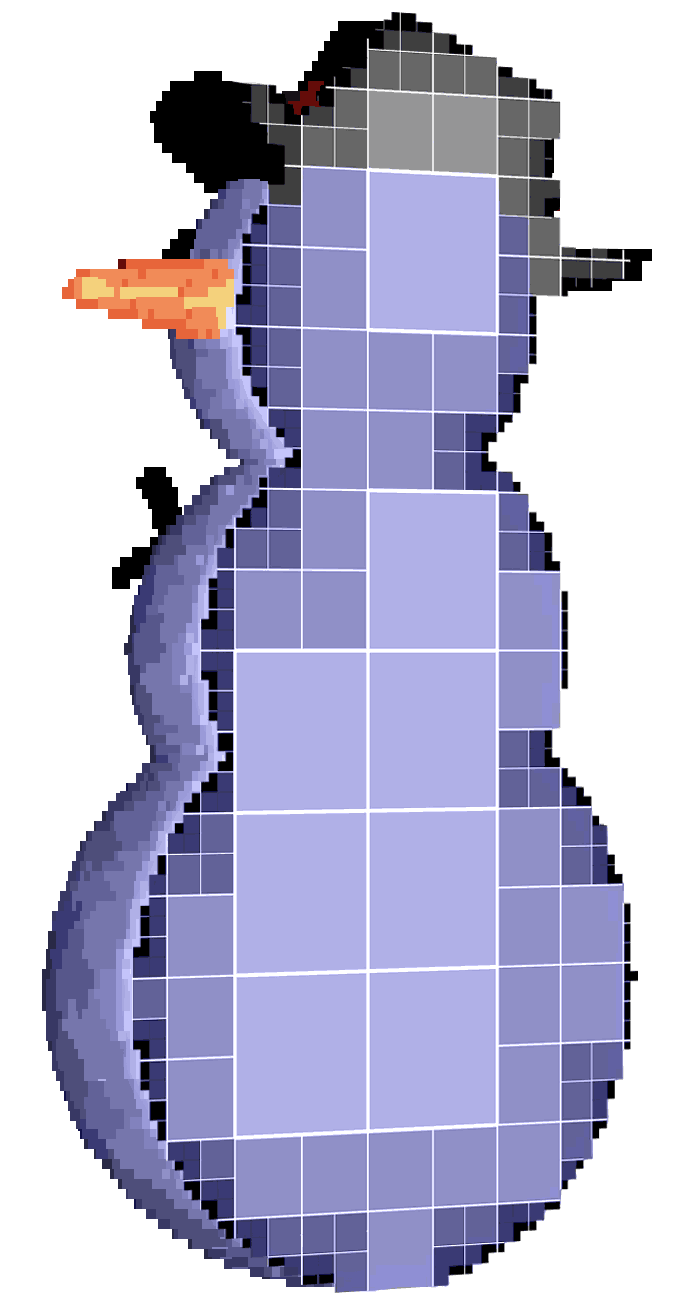
\includegraphics[scale=0.2]{obrazky-figures/svo_snowman.png}	\captionsetup{justification=centering}
	\boldcaption[\textbf{Reprezentace modelu pomocí sparse octree.}]{ V obrázku je vidět, že oblasti pro které není nutné udržovat detail jsou velice úsporné.}
	\label{fig:svo_example}
\end{figure}

Pro průchod octree je tedy nutné využít datové struktury zásobník. Kdykoli, kdy algoritmus postoupí do nižší úrovně stromu (\textit{PUSH}), je potenciálně uložen předchozí rodič. Pokud je současná větev nevhodná pro další výpočty, je vyvolán \textit{POP} a tím se posune algoritmus v hierarchii výše. 

Při postupu v hierarchii níže dochází k volbě vhodného potomka. Volba je založena na vyhodnocení $t_x$, $t_y$ a $t_z$ a jejich porovnání s $tc_{min}$.

Tuto metodu autor zvolil pro výpočet primárních paprsků kvůli vysoké přesnosti a poměrně nízké výpočetní náročnosti tohoto algoritmu. Metoda pro výpočet sekundárních paprsků je popsána v následující sekci.



\subsection{Light field probes}\label{sec:lfp_design}
Light field probes byly již krátce představeny v sekci \ref{sec:ray_tracing}. Každá sonda je reprezentována svou pozicí a texturou, která obsahuje následující informace:
\begin{itemize}
 \item Radiální vzdálenost ke geometrii.
 \item Normálu.
 \item Informace o materiálu, barvě či jiná data využitá v další práci se sondami.
\end{itemize}

Tato textura má velikost 1024x1024 a každý texel reprezentuje dvě float hodnoty (\texttt{rg32f}). Vzhledem k tomu, že paměťová náročnost je poměrně vysoká, je nutné ukládaná data nějakým vhodným způsobem komprimovat. Radiální vzdálenost ke geometrii je možné logaritmovat pro zachování vyšší přesnosti pro bližší objekty a také kvantovat na snížení paměťové náročnosti. Logaritmizace a linearizace hloubky obsahuje rovnice \ref{eq:depth_econde_decode},

\begin{equation} \label{eq:depth_econde_decode}
	\begin{gathered}
		encoded\_depth = \frac{log(C \cdot depth + 1)}{log(C \cdot Far)}\\
		decoded\_depth = \frac{(C \cdot Far + 1)^{encoded\_depth} - 1}{C}
	\end{gathered}
\end{equation}

kde $C$ je konstanta modifikující rozložení přesnosti, často nastavena na 1, $depth$ je hloubka a $Far$ je maximální vzdálenost. Po logaritmizaci je hodnota transformována na 16 bitů a uložena do textury sondy.

Dalším parametrem jsou normály. Ty lze zakódovat na 2 float hodnoty mnoha metodami, jak je uvedeno v \cite{Cigolle2014ASO}. Autor zvolil metodu projekce na osmistěn. Po projekci jsou složky výsledného vektoru kvantovány na 8 bitů, čímž je celková potřebná paměť pro uložení těchto hodnot snížena na 16 bitů. Rovnice \ref{eq:normal_encode} popisuje zakódování normály a \ref{eq:normal_decode} její dekódování.

\begin{equation} \label{eq:normal_encode}
	\begin{gathered}
		\vec{p} = normal_{xy} \frac{1}{|normal_x| + |normal_y| + |normal_z|} \\
		\vec{encoded\_normal} = \begin{cases}
            (1 - |p_{yx}|) \cdot sign(\vec{p}),& \text{pokud } normal_z \leq 0.0\\
            \vec{p},              & \text{jinak}
        \end{cases}\\
	\end{gathered}
\end{equation}

Kde $normal$ je normála, $p$ je pomocný vektor k projekci a $encoded\_normal$ je zakódovaná normála.

\begin{equation} \label{eq:normal_decode}
	\begin{gathered}
	    z = 1 - |encoded\_normal_x| - |encoded\_normal_y|\\
	    \vec{v} = \langle encoded\_normal_{xy}, z \rangle\\
		\vec{decoded\_normal} = \begin{cases}
            \langle (1 - |v_{yx}|) \cdot sign(v_{xy}), v_z \rangle,& \text{pokud } v_z < 0.0\\
            normalize(\vec{v}),              & \text{jinak}
        \end{cases}\\
	\end{gathered}
\end{equation}

Kde $encoded\_normal$ je zakódovaná normála, $z$ je vypočtená třetí složka výsledné normály, $v$ je pomocný vektor a $decoded\_normal$ je dekódovaná normála.

Poslední položkou uloženou v textuře sondy je radiance. Pro případné další rozšíření je uložena ve formátu \texttt{R11G11B10} pro podporu HDR.

Jelikož sonda reprezentuje světelné pole ve svém okolí jakožto kouli, je nutné data nějakým způsobem transformovat na texturu, tedy rovinu. Toho lze dosáhnout mapováním koule na osmistěn a následné projekce na rovinu, jak je znázorněno na obrázku \ref{fig:octahedral_wrap}. Pro tuto projekci a její inverzní operaci je možné využít rovnic \ref{eq:normal_encode} a \ref{eq:normal_decode}.

\begin{figure}[H]
	\centering
	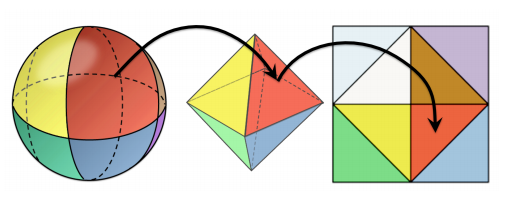
\includegraphics[scale=2]{images/octahedral_wrap.png}
	\captionsetup{justification=centering}
	\boldcaption[\textbf{Vizualizace projekce koule na osmistěn a následně na rovinu.}]{ }
	\label{fig:octahedral_wrap}
\end{figure}

Výpočet informací o geometrii je prováděn pomocí ray tracingu představeném v sekci \ref{sec:rendering}. Na obrázku \ref{fig:probe_in_scene} je ukázka dat jedné ze sond.


\begin{figure}[H]
	\centering
	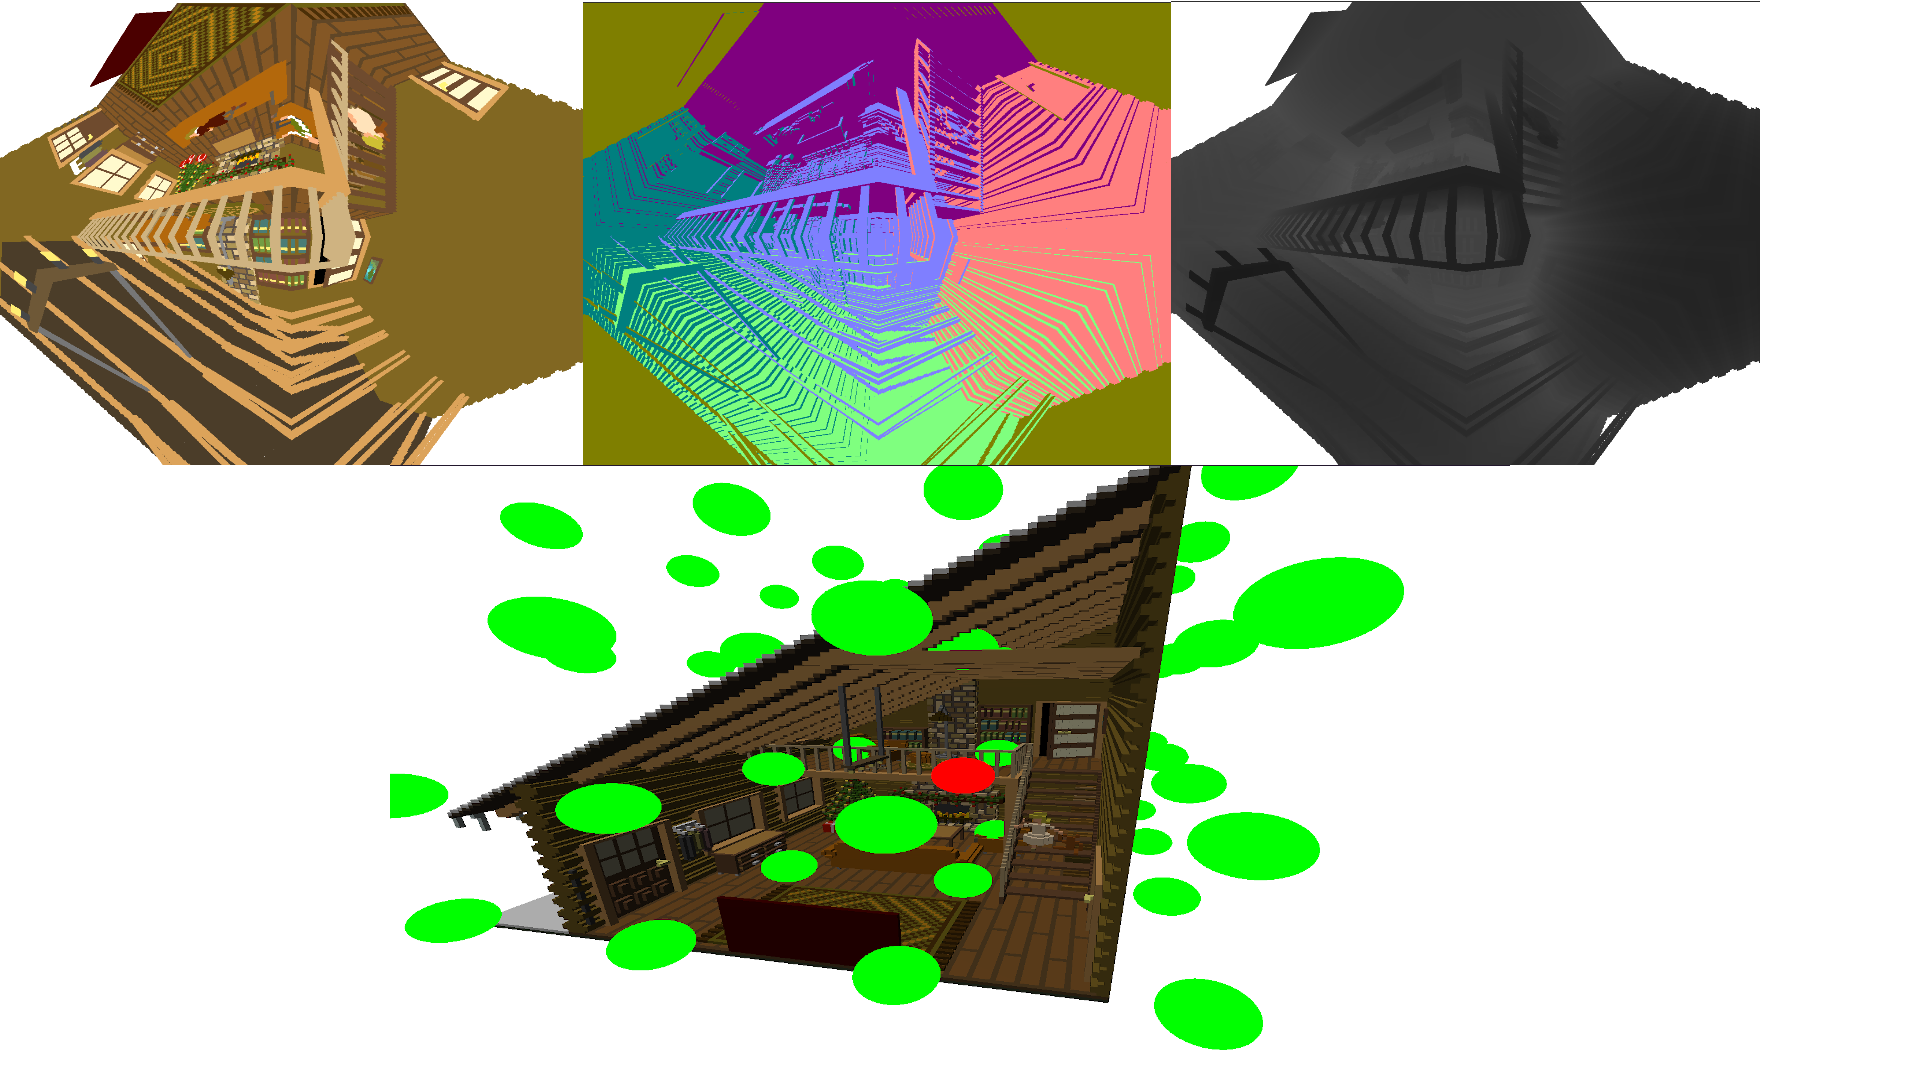
\includegraphics[scale=1]{images/probe_with_scene.png}
	\captionsetup{justification=centering}
	\boldcaption[\textbf{Vizualizace dat uložených pro sondu.}]{ V horní polovině obrázku je vyobrazena radiance, normály a hloubka. Dolní část ukazuje pozici sondy ve scéně (červená).}
	\label{fig:probe_in_scene}
\end{figure}

\subsection{Renderování scény pomocí light field probes}\label{sec:render_lfp}
Pomocí atlasu textur, který byl vytvořen pro všechny sondy pokrývající scénu, je možné provádět trasování paprsku. Tato metoda byla popsána v publikaci \cite{light_field_probes}. Díky radiální vzdálenosti a normálám zakódovaných v sondách je možné vypočítat průsečíky nesouvislých paprsků. 

V prvé řadě je nutné pro paprsek vybrat vhodnou sondu, ve které zahájíme jeho sledování. Pokud tato sonda není schopná poskytnout nám jistý \textit{miss} (minutí scény) nebo \textit{hit} (protnutí scény) je nutné vybrat alternativní sondu, která má nějakou šanci paprsek sledovat. Sledování paprsku v rámci jedné sondy tedy vrací tři stavy:
\begin{itemize}
    \item \textit{miss} -- minutí scény
    \item \textit{hit} -- průsečík se scénou
    \item \textit{unknown} -- neznámý výsledek
\end{itemize}

Stav \textit{unknown} nastane pouze v případě, kdy paprsek prochází ve větší vzdálenosti, než jaká je v dané pozici radiální hloubka. Jinými slovy: pokud sonda "ví", že nemá dostatečné informace o scéně v dané pozici, nemůže být paprsek spolehlivě vyhodnocen pouze pomocí informací z této sondy. 

Sledování paprsku začíná převedením jeho počátku do prostoru sondy. Následně je paprsek transformován pomocí projekce na osmistěn do souřadnic textury. Dochází tedy k transformaci přímky z $R^3$ do křivky v $R^2$. Tato křivka má až čtyři segmenty, kde každý segment leží v jiné stěně osmistěnu. Následně algoritmus postupuje po jednotlivých texelech nacházejících se na této křivce a vyhodnocuje, jestli dochází k průsečíku pomocí porovnávání uložené hloubkové mapy se vzdáleností paprsku k sondě. Pokud je paprsek ve stejné vzdálenosti nebo je dále, dochází k průsečíku nebo paprsek prochází za geometrií. Algoritmus pro výpočet průsečíku obsahuje algoritmus \ref{alg:single_probe_trace}. 

\begin{center}
	\begin{czechalgorithm}[H] \label{alg:single_probe_trace}
	    segments = compute\_segments(ray, probe)\\
	    \ForEach{segment in segments}{
	        coords\_on\_segment = create\_coords(segment)\\
	        \ForEach{coord in coords\_on\_segment}{
	            state = compare\_ray\_distance\_to\_radial(ray, coord, probe)\\
	            \uIf{state == HIT}{
	                \KwRet (HIT, coord)
	            }
	            \uIf{state == HIDDEN\_BEHIND\_SURFACE}{
	                \KwRet (UNKNOWN, coord) 
	            }
	        }
	    }
	    \KwRet (MISS, last\_point\_on\_segments)
		\caption{Sledování paprsku v rámci jedné sondy}
	\end{czechalgorithm}
\end{center}

Pro urychlení tohoto algoritmu je pro každou sondu vytvořena další textura, která má 16krát menší velikost -- tedy 64x64 -- a ve které jsou uloženy v každém texelu nejbližší radiální vzdálenosti. Jedná se prakticky o mipmapu. Při procházení pixelů segmentů tedy není nutné provádět algoritmus na maximálním rozlišení, čímž dochází k výraznému zrychlení. Pouze při nalezení potenciálního průsečíku je trasování prováděno na vysokém rozlišení. Na obrázku \ref{fig:lfp_trace} je vizualizace průchodu paprsku jednou sondou.

\begin{figure}[H]
	\centering
	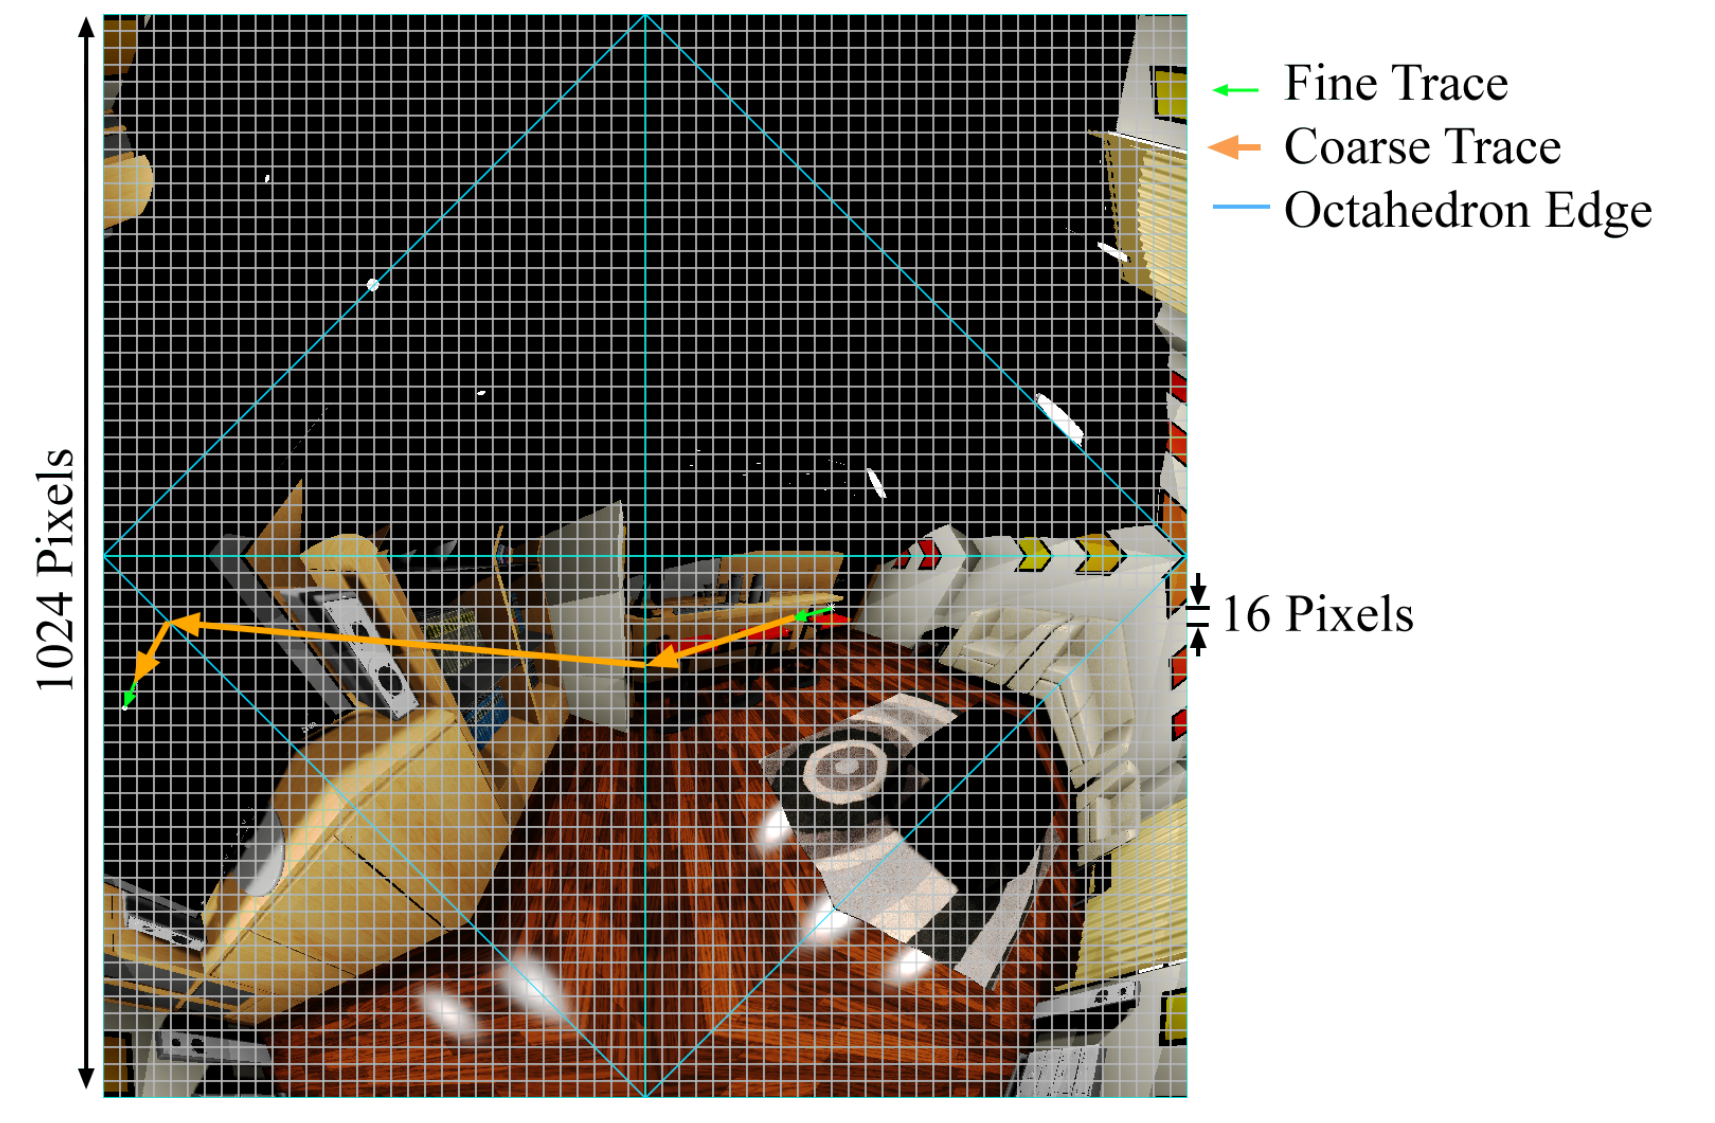
\includegraphics[scale=0.85]{images/lfp_trace.png}
	\captionsetup{justification=centering}
	\boldcaption[\textbf{Sledování paprsku v textuře sondy.}]{ Oranžová část paprsku je prováděna pouze na textuře s nižším rozlišením, zelená je prováděna na vysokém rozlišení pokud dochází k detekci potenciálního průsečíku. Převzato z Real-Time Global Illumination using Precomputed Light Field Probes \cite{light_field_probes}.}
	\label{fig:lfp_trace}
\end{figure}

\paragraph{Výběr sondy.} Nejdůležitějším krokem je výběr vhodné sondy pro zahájení algoritmu. Jedním možným řešením je výběr sondy čistě podle vzdálenosti k počátku paprsku, což doporučuje taktéž článek \cite{light_field_probes}, s tím, že výběr dalších sond se řídí pořadím uvedeným v obrázku \ref{fig:lfp_cube}. Pokud se paprsek nenachází v jiné skupině sond po dokončení průchodu této skupiny, je hledání ukončeno jako neúspěšné, jinak je prováděno v nové skupině. V případě autorova řešení docházelo k velkému množství \textit{unknown} výsledků a proto se rozhodl implementovat jiné řešení. 

\begin{figure}[H]
	\centering
	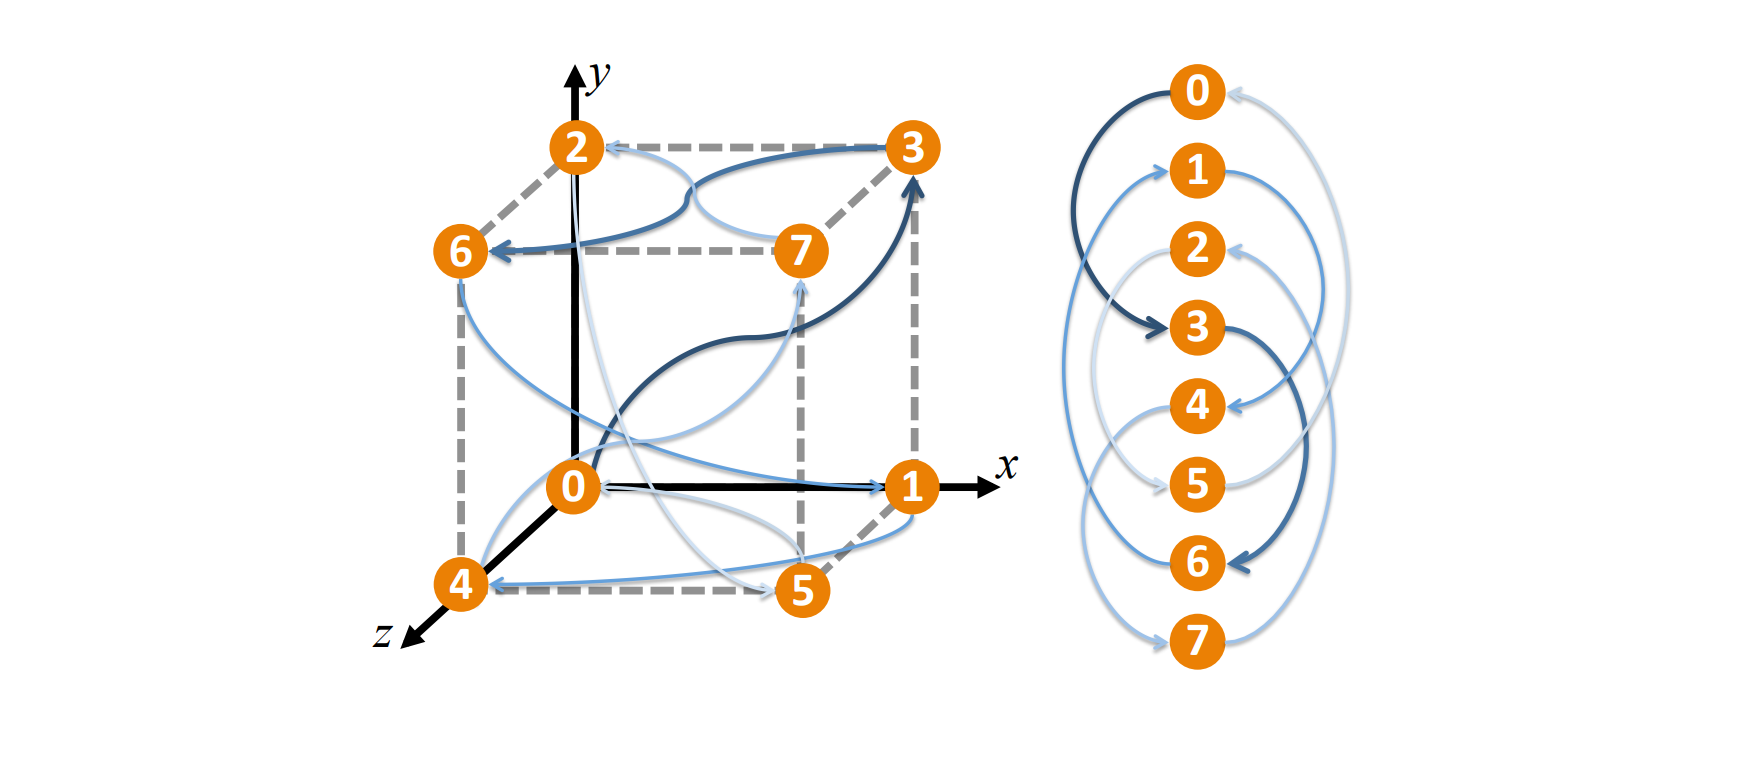
\includegraphics[scale=1]{images/probe_cube.png}
	\captionsetup{justification=centering}
	\boldcaption[\textbf{Pořadí výběru sondy pro lokální skupinu.}]{Převzato z Real-Time Global Illumination using Precomputed Light Field Probes \cite{light_field_probes}.}
	\label{fig:lfp_cube}
\end{figure}

Namísto výběru sondy tak, jak je popsáno v předchozím odstavci, je možné rozdělit prostor, jenž je sondami sledován, na voxelové pole (mřížku). Toto pole obsahuje pro každý voxel až čtyři sondy, pro které se daný voxel vyskytuje blíže, než je jejich radiální vzdálenost ke scéně. Namísto výběru nejbližší sondy je tedy sonda vybrána dle toho, ve kterém voxelu se paprsek současně nachází. Sledování je ukončeno pouze tehdy, pokud žádná ze sond uložená v tomto poli nenalezla řešení a sledovaný bod paprsku se neposunul do jiného voxelu. 

\begin{center}
	\begin{czechalgorithm}[H] \label{alg:light_field_trace}
	    result = UNKNOWN\\
	    \While{result == UNKNOWN}{
	        probe = select\_probe\_from\_voxel\_field(ray)\\
	        \uIf{\Not is\_valid\_probe(probe)}{
	            break
	        }
	        (result, endpoint) = trace\_single\_probe(ray, probe)\\
	        ray.origin = endpoint
	    }
	    \KwRet result
		\caption{Sledování paprsku skrze light field}
	\end{czechalgorithm}
\end{center}

Na obrázku \ref{fig:lfp_scene_render} je zobrazena scéna vykreslená čistě pomocí výše popsané metody.

\begin{figure}[H]
	\centering
	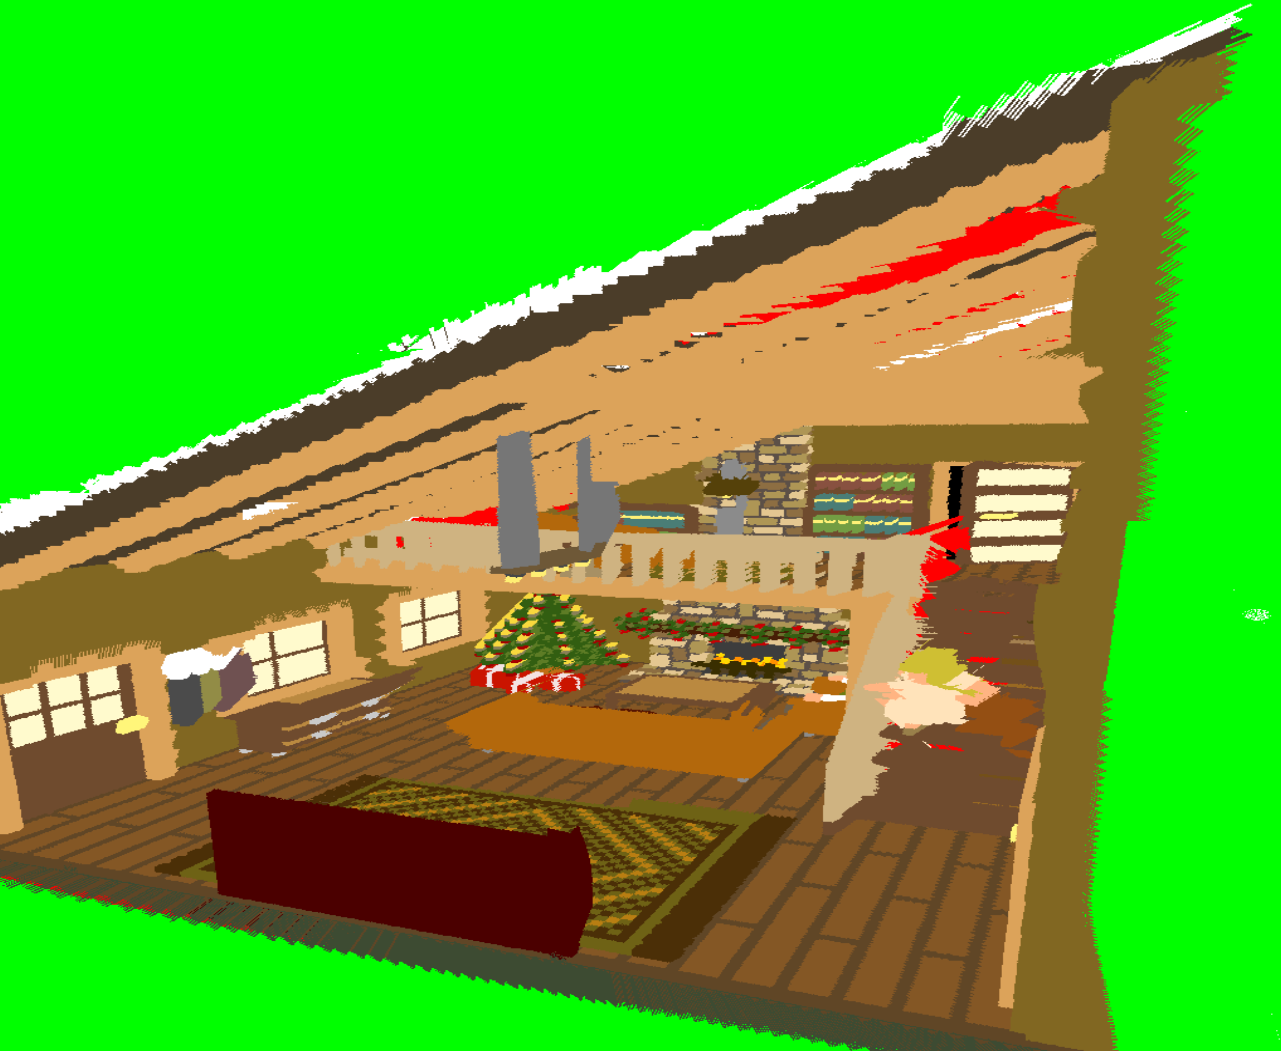
\includegraphics[scale=1]{images/probe_scene_render.png}
	\captionsetup{justification=centering}
	\boldcaption[\textbf{Scéna vykreslena algoritmem sledování paprsku skrze light field.}]{ Zelené oblasti značí \textit{miss}, červené \textit{unknown}. Je vidět, že dochází k mnoha nepřesnostem a ve scéně, kde je spousta objektů dochází ke vzniku míst, kde sondy nenaleznou řešení.}
	\label{fig:lfp_scene_render}
\end{figure}

\subsection{Nepřímé osvětlení}\label{sec:indirect}
Původním záměrem autora bylo využít výše popsané sondy k výpočtu sekundárních paprsků ve scéně online, ale ukázalo se, že pro takový přístup je tato metoda příliš pomalá. Bylo tedy nutné vymyslet alternativní řešení. 

Pro již zmíněnou metodu se nabízí modifikace, která by umožnila přidat funkčnost nepřímého osvětlení tak, že do atlasu textur sond je vypočteno nepřímé osvětlení při jejich inicializaci a posléze jsou aplikovány při renderování scény.  K výpočtu je použit ray tracing implementovaný pomocí metody popsané v první části sekce. Pro každý texel, který reprezentuje difuzní materiál, je vysláno několik paprsků z místa prvního průsečíku scény. Tyto paprsky se dále odráží ve scéně a sbírají světlo z vnějších zdrojů/emitujících materiálů.


\begin{figure}[H]
	\centering
	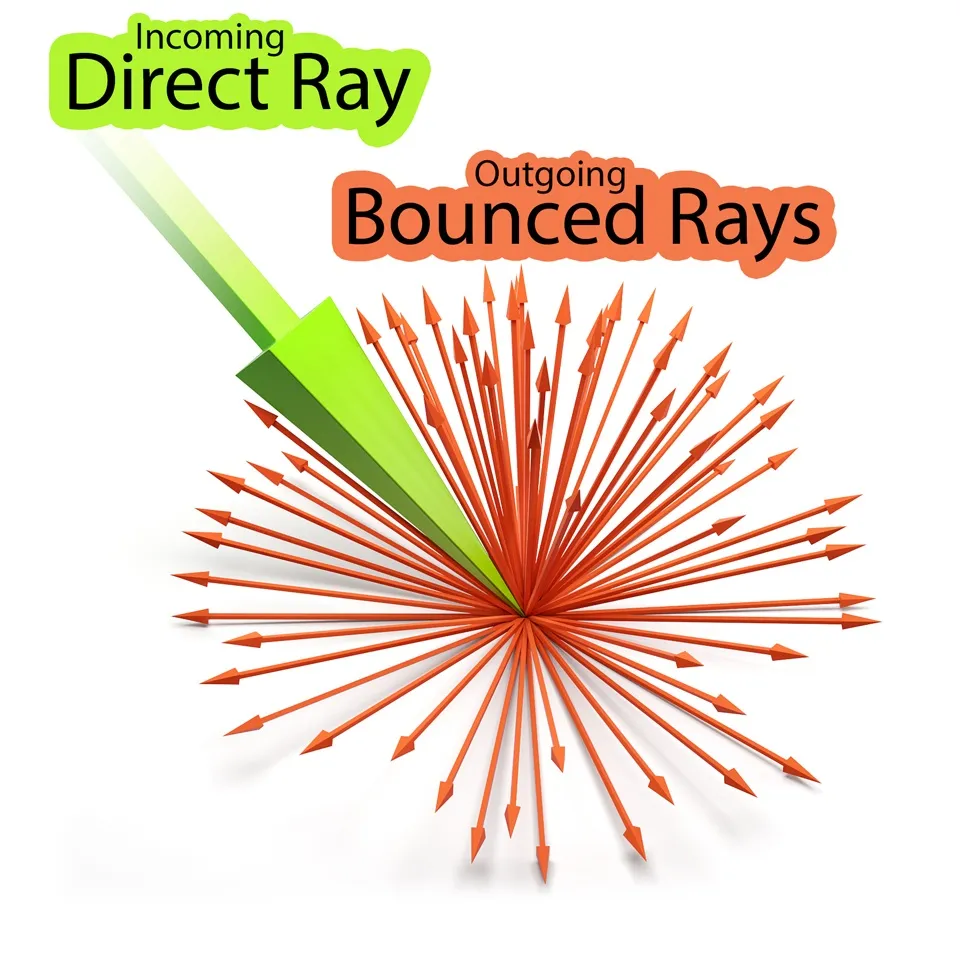
\includegraphics[scale=0.15]{images/diffuse_bounce.png}
	\captionsetup{justification=centering}
	\boldcaption[\textbf{Paprsky odražené z difuzního materiálu.}]{Převzato z \url{https://renderstuff.com/tutorials/indirect-illumination-in-v-ray-tutorial-176/}.}
	\label{fig:diffuse_rays}
\end{figure}


Jelikož informace o materiálech poskytované zdrojovými modely jsou poměrně stručné, odraz paprsku je prováděn náhodně v polokouli určené normálou, jak je demonstrováno na obrázku \ref{fig:diffuse_rays}. Výpočet příspěvku osvětlení je popsán v algoritmu \ref{alg:bounce_bake}.

\begin{center}
	\begin{czechalgorithm}[H] \label{alg:bounce_bake}
	    result = vector(1, 1, 1)\\
	    \For{i in range(0, MAX\_BOUNCES)}{
	        (is\_hit, position, normal, material\_type) = trace\_ray(ray)\\
	        \uIf{\Not is\_hit}{
	            break
	        }
	        \uIf{material\_type == DIFFUSE}{
	            result *= attentuation\\
	            ray.origin = position\\
	            ray.direction = random\_point\_on\_hemisphere(normal)
	        }
	        \uIf{material\_type == METALLIC}{
	            ray = bounce\_ray\_for\_metallic(ray, position, normal)\\
	        }
	        \uIf{material\_type == EMIT}{
	            add\_emissive\_light(result)\\
	            break
	        }
	    }
	    \KwRet result
		\caption{Výpočet nepřímého osvětlení}
	\end{czechalgorithm}
\end{center}

\begin{figure}[H]
	\centering
	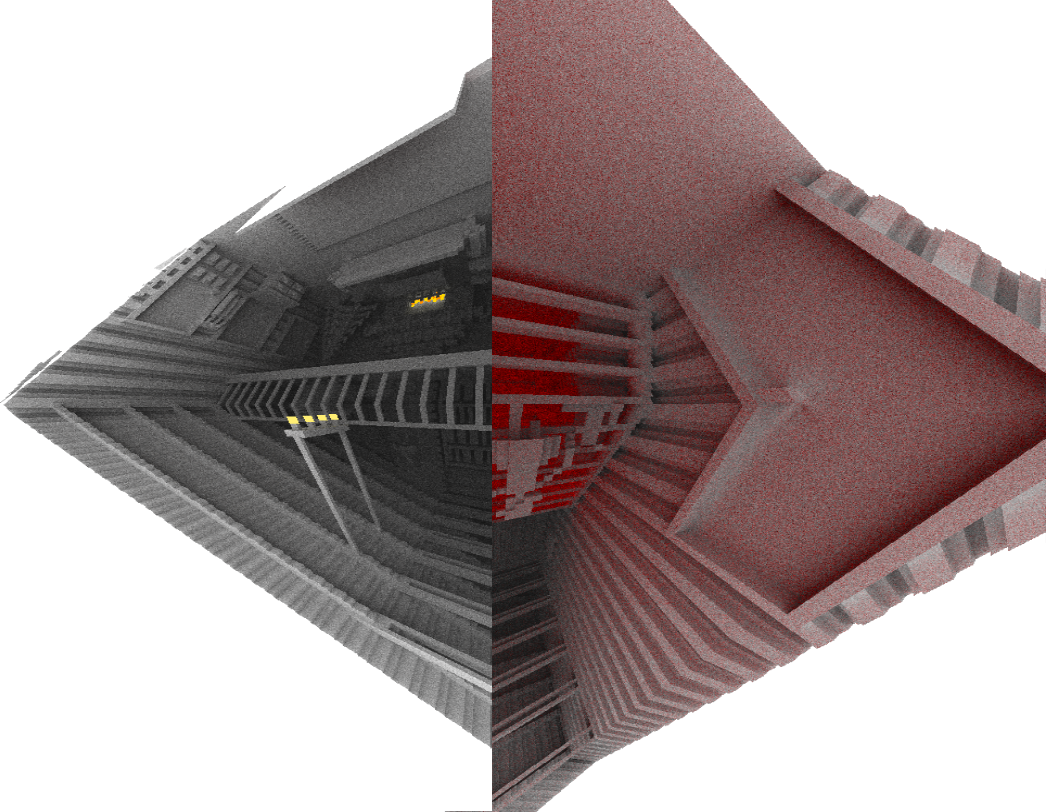
\includegraphics[scale=1]{images/indirect_probe.png}
	\captionsetup{justification=centering}
	\boldcaption[\textbf{Textura sondy obsahující informace o nepřímém osvětlení.}]{ Na levé straně je zdrojem pouze vnější osvětlení, vpravo je vidět vliv emitujícího materiálu. }
	\label{fig:diffuse_rays}
\end{figure}


\section{Struktura vykreslovacího řetězce}

K vykreslení finálního snímku je samozřejmě potřeba zkombinovat metody popsané v předchozí sekci. Jak je vidět z obrázku \ref{fig:lfp_scene_render}, používat light field probes jako primární vykreslovací algoritmus není vhodné, jelikož dochází k vzniku velkého množství nepřesností. Z tohoto důvodu je pro první fázi využit ray tracing ve sparse voxel octree -- popsáno v sekci \ref{sec:svo_design}.

\begin{figure}[H]
	\centering
	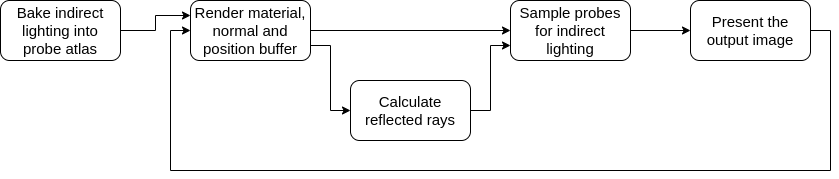
\includegraphics[scale=0.5]{images/my_render_pipeline.png}
	\captionsetup{justification=centering}
	\boldcaption[\textbf{Postup vykreslování jednotlivých snímků.}]{ Výpočet nepřímého osvětlení pro sondy je prováděn pouze při inicializaci, případě jako reakce na požadavek uživatele. }
	\label{fig:gbuffer_contents}
\end{figure}

Před zahájením vykreslování snímku je nutné připravit atlas sond. Pro "online" výpočet sekundárních paprsků by bylo dostačující připravit do atlasu radianci, normály a hloubku, vzhledem k vysoké časové náročnosti tato metoda nebude použita. Namísto radiance je tedy v atlasu sond uložen příspěvek nepřímého osvětlení (obrázek \ref{fig:diffuse_rays}). Tento proces, s ohledem na jeho náročnost, může trvat delší dobu, ale je dostačující ho provést pouze při inicializaci scény. Celý řetězec je na obrázku \ref{fig:gbuffer_contents}.

Další krok je již opakován periodicky pro každý snímek. Pomocí sparse voxel octree je vykreslen buffer, který obsahuje informace o místě průsečíku scény, index materiálu a normálu -- tento buffer je zobrazen v obrázku \ref{fig:gbuffer_contents}. 

Následně je na základě hodnot v bufferu dohledáno ze sond a jejich atlasu nepřímé osvětlení. Díky použití mřížky k urychlení nalezení potenciálně vhodné sondy (sekce \ref{sec:render_lfp}) lze očekávat, že tato operace nezabere příliš mnoho času. Také je možné, že pro daný fragment existuje několik různých zdrojů dat o nepřímém osvětlení, jelikož tato data mohou být uložena ve více sondách, čímž se efektivně výrazně zvyšuje počet sekundárních paprsků. V tomto kroku paralelně též probíhá výpočet odražených paprsků pro metalické materiály.


\begin{figure}[H]
	\centering
	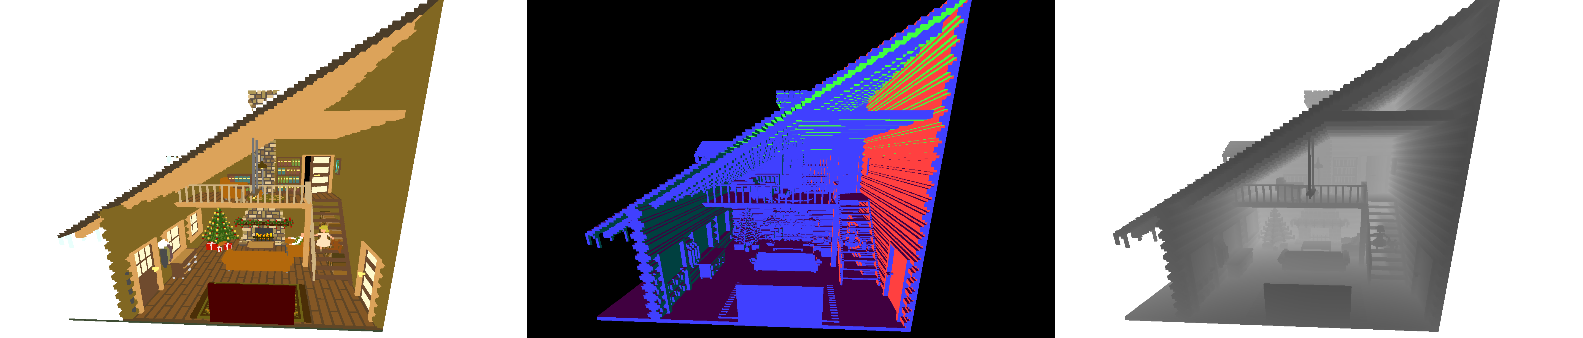
\includegraphics[scale=1]{images/gbuffer_render.png}
	\captionsetup{justification=centering}
	\boldcaption[\textbf{Složky bufferu vykreslené na začátku rámce.}]{ Zleva se jedná o index materiálu (zobrazeno jako barva materiálu), normály, pozici ve světe (zobrazeno jako hloubka). }
	\label{fig:gbuffer_contents}
\end{figure}


\chapter{Implementace}
\label{implementace}

Tato kapitola obsahuje seznam použitých nástrojů a knihoven. Popisuje implementaci knihoven vytvořených při práci na praktické části tohoto projektu, také algoritmy použité ke tvorbě octree a uživatelské rozhraní demonstrační aplikace.

\section{Použité knihovny a nástroje}
Pro implementaci autor zvolil jazyk \texttt{c++}, standard 20\footnote{\url{https://en.cppreference.com/w/cpp/20}}, kvůli autorově pokročilé znalosti tohoto jazyka a také jako možnost procvičit si nově přidané funkce v~poslední revizi. Pro překlad projektu byl použit \texttt{CMake}\footnote{\url{https://cmake.org/}} v~kombinaci s~\texttt{Ninja}\footnote{\url{https://ninja-build.org/}} a package management nástroji \texttt{CPM.cmake}\footnote{\url{https://github.com/TheLartians/CPM.cmake}} a \texttt{Hunter}\footnote{\url{https://hunter.readthedocs.io/en/latest/}}. Jako vývojové prostředí bylo použito \texttt{CLion}\footnote{\url{https://www.jetbrains.com/clion/}}. Kód shaderů je vytvořen v~GLSL\footnote{\url{https://www.khronos.org/opengl/wiki/Core_Language_(GLSL)}}. Při práci na projektu byly taktéž využity tyto knihovny třetích stran:

\begin{itemize}
	\begin{AutoMultiColItemize}
		\item \texttt{spdlog}\footnote{\url{https://github.com/gabime/spdlog}}
		\item \texttt{range-v3}\footnote{\url{https://github.com/ericniebler/range-v3}}
		\item \texttt{magic\_enum}\footnote{\url{https://github.com/Neargye/magic_enum}}
		\item \texttt{argparse}\footnote{\url{https://github.com/p-ranav/argparse}}
		\item \texttt{toml++}\footnote{\url{https://marzer.github.io/tomlplusplus/}}
		\item \texttt{backward-cpp}\footnote{\url{https://github.com/bombela/backward-cpp}}
		\item \texttt{cppcoro}\footnote{\url{https://github.com/lewissbaker/cppcoro}}
		\item \texttt{\{fmt\}}\footnote{\url{https://github.com/fmtlib/fmt}}
		\item \texttt{stb}\footnote{\url{https://github.com/nothings/stb}}
		\item \texttt{glm}\footnote{\url{https://github.com/g-truc/glm}}
		\item \texttt{Dear ImGui}\footnote{\url{https://github.com/ocornut/imgui}}
	\end{AutoMultiColItemize}
\end{itemize}

Dále byly využity následující nástroje pro statickou analýzu kódu, formátování atp.:
\begin{itemize}
	\begin{AutoMultiColItemize}
		\item \texttt{cppcheck}\footnote{\url{http://cppcheck.sourceforge.net/}}
		\item \texttt{cpplint}\footnote{\url{https://github.com/cpplint/cpplint}}
		\item \texttt{sanitisers}\footnote{\url{https://github.com/google/sanitizers}}
		\item \texttt{valgrind}\footnote{\url{https://valgrind.org/}}
		\item \texttt{Ccache}\footnote{\url{https://ccache.dev/}}
		\item \texttt{clang-format}\footnote{\url{https://clang.llvm.org/docs/ClangFormat.html}}
	\end{AutoMultiColItemize}
\end{itemize}

\section{Knihovna pf\_common}
Knihovna poskytující často používané funkce:
\begin{itemize}
	\item \texttt{Concept}y a další nástroje pro template meta programování a statický polymorfimus.
	\item Jednoduché coroutines (\texttt{iota}, \texttt{range}...)
	\item Implementace výjimek se stack trace reporting.
	\item Některé idiomy \texttt{c++} -- \texttt{RAII}, \texttt{Visitor}...
	\item Funkce pro binární serializaci dat a práci s~binárními daty.
	\item Obecné geometrické funkce, které nejsou poskytnuty v \texttt{glm}.
	\item Funkce pro rozšíření možnosti využití \texttt{enum}.
	\item Mnoho dalších...
\end{itemize}

Je implementována jako header-only knihovna\footnote{\url{https://en.wikipedia.org/wiki/Header-only}}.

\section{Knihovna pf\_glfw\_vulkan}
Tato knihovna poskytuje dvě základní funkce:
\begin{itemize}
	\item vytvoření a správa okna pomocí \texttt{GLFW}\footnote{\url{https://www.glfw.org/}}
	\item komunikace s~GPU za pomocí \texttt{Vulkan API}\footnote{\url{https://www.khronos.org/vulkan/}}
\end{itemize}

Třída \texttt{GlfwWindow} umožňuje instanciaci GLFW knihovny a také komunikaci za pomocí událostí, které knihovna programu předává. Zprostředkovává tak uživateli možnost interagovat s aplikací za pomocí periferních zařízení (myš a klávesnice). Tato třída splňuje concept\footnote{\url{https://en.cppreference.com/w/cpp/language/constraints}} \texttt{Window}, který je také obsažen v~knihovně. Za pomoci \texttt{Window} je implementována komunikace mezi \texttt{Vulkan} a okenním systémem. Díky tomuto rozdělení si může uživatel vytvořit komunikační vrstvu mezi knihovnou a jiným okenním systémem, jako například \texttt{SDL}\footnote{\url{https://www.libsdl.org/}}. Pro tento účel implementuje knihovna vlastní notifikační systém událostí ve třídě \texttt{EventDispatchImpl}, který výrazně usnadňuje případnou implementaci s jiným okenním backendem.

Část knihovny pro interakci s~\texttt{Vulkan} je o~poznání rozsáhlejší. Při návrhu knihovny byl kladen zřetel především na její jednoduchost a zároveň bezpečnost jejího užívání. Z~tohoto důvodu je uvnitř hojně využito \texttt{std::shared\_ptr}. Vzhledem k~tomu, že ve \texttt{Vulkan} je nutné často vytvářet objekty v~závislosti na některém z dříve vytvořených (například \texttt{vk::Instance} $\longrightarrow$ \texttt{vk::PhysicalDevice} $\longrightarrow$ \texttt{vk::Device}), si v~sobě každý nově vytvořený potomek ukládá ukazatel na svého "rodiče". To zaručuje, že nemůže dojít k~uvolnění objektů omylem, v případě, že budeme používat některého z~jeho potomků.

Knihovna obsahuje vlastní verzi velkého množství \texttt{Vulkan} objektů a zároveň je plně typově bezpečná. Příkladem může být přístup do \texttt{vk::Buffer}, kdy k~datům přistupujeme pomocí mapovacího objektu, který ve velké míře využívá template funkcí pro kontrolu offsetu a správné práce s~pamětí.

Všechny objekty jsou potomkem \texttt{VulkanObject}, což je rozhraní, které poskytuje základní debug informace o~objektu. Vytváření objektů je vždy prováděno pomocí \texttt{struct} konfiguračních dat. Předpokládá se užití \texttt{designated initialisers}\footnote{\url{https://en.cppreference.com/w/cpp/language/aggregate_initialization#Designated_initializers}}. Ukázka vytvoření logického zařízení:

\begin{lstlisting}[language=C++, caption={Tvorba logického zařízení}]
// tvorba instance vynechana kvuli velkemu mnozstvi argumentu
device = instance->selectDevice(DefaultDeviceSuitabilityScorer());
surface = instance->createSurface(window);
logicalDevice = device->createLogicalDevice({
    .id = "dev1",
    .deviceFeatures = vk::PhysicalDeviceFeatures{},
    .queueTypes = {vk::QueueFlagBits::eCompute},
    .presentQueueEnabled = true,
    .requiredDeviceExtensions = {VK_KHR_SWAPCHAIN_EXTENSION_NAME},
    .validationLayers = getValidationLayers(),
    .surface = *surface});
\end{lstlisting}

Pro objekty, u~nichž by konfigurační struktura vyžadovala nadměrně velké množství argumentů, jsou v~knihovně dostupné builder třídy, například \texttt{GraphicsPipelineBuilder} nebo \texttt{RenderPassBuilder}.

Součástí knihovny je též rozhraní pro kompilaci shader souborů z disku nebo paměti.



\section{Knihovna pf\_imgui}\label{sec:pf_imgui}
\texttt{pf\_imgui} je event-driven UI knihovna postavena na Dear Imgui. Cílem je zjednodušení práce při vytváření uživatelského rozhraní a také přidání některých funkcí. Funkce, které jsou nad rámec Dear Imgui přidané, jsou:

\begin{itemize}
	\item Pozorování změn hodnot pomocí callback funkcí (observer pattern).
	\item Ukládání hodnot do konfiguračního souboru. Tyto změny jsou načteny vždy při zapnutí programu.
	\item Některé elementy navíc, například \texttt{Memo}.
\end{itemize}

Knihovna je postavena nezávisle na renderovacím backendu, v repository je poskytnut backend pro Vulkan a GLFW. Pro vlastní použití je nutné rozšířit hlavní objekt \texttt{ImGuiInterface} a přidat volání do backendu své volby. Například pro Vulkan by se mohlo jednat o~jednoduchou funkci přidání draw command do \texttt{vk::CommandBuffer}. V~knihovně je obsaženo podstatné množství elementů, přičemž jsou implementovány wrappery pro všechny elementy dostupné v~Dear Imgui. Také jsou přidány grafy z~knihoven \texttt{ImGuiFlameGraph}\footnote{\url{https://github.com/bwrsandman/imgui-flame-graph}}, \texttt{implot}\footnote{\url{https://github.com/epezent/implot}} a možnost interagovat se soubory na disku pomocí \texttt{ImGuiFileDialog}\footnote{\url{https://github.com/aiekick/ImGuiFileDialog}}.

V knihovně je také implementováno podstatné množství layoutů -- grid layout, anchor layout a další.

Přidání vlastních elementů do knihovny je velice primitivní. Připravená rozhraní pokrývají spoustu potenciální funkčnosti, a to například včetně \textit{drag and drop} a rozhraní pro nastavení stylu/ barvy elementu. 

Kupříkladu implementace \texttt{CheckBox} vyžaduje pouze \textasciitilde10 řádků kódu -- nepočítaje deklarace funkcí a tělo konstruktoru -- s~tím, že dědí z~\texttt{ItemElement}, \texttt{Labellable}, \texttt{Savable}, \texttt{ValueObservable<bool>}, \texttt{ColorCustomizable<...>} a \texttt{StyleCustomizable<...>}.

Ukázka vytvoření tlačítka, které reaguje na kliknutí otevřením dialogu pro výběr \texttt{txt} souboru:

\begin{lstlisting}[language=C++, caption={Vytvoření tlačítka pro výběr souboru}]
imgui.createChild<Button>("btn_id", "Open file")
    .addClickListener([&imgui] {
        imgui.openFileDialog("Select file", 
            {.ext = {"txt"}, .description = "txt  files"}, 
            [] (const auto &files) {
                for (const auto &file : files) { print(file); }
            }, [] { print("No file selected"); });
    }
\end{lstlisting}

\section{Struktura programu}
Na obrázku \ref{fig:program_flow} je diagram hlavní struktury programu. V diagramu jsou zobrazeny pouze větší části programu, kdy každá část je závislá na té předchozí. Prvním krokem je načtení konfigurace, která je blíže popsána v sekci \ref{sec:demo_app}. Následně dochází k inicializaci okenního systému za pomocí knihovny \texttt{pf\_glfw\_imgui}, stejná knihovna je využita v inicializaci Vulkan. Dále je vybudováno uživatelské rozhraní s tím, že jsou mu přiřazeny všechny potřebné funkce. Po tomto nastavení se program dostává do hlavní smyčky, kde jsou krom interakce uživatele s UI a kamerou prováděny dvě důležité operace -- načítání modelů (částečně prováděno na separátním vlákně) a vykreslování společně s prezentací obrázku.

\begin{figure}[H]
	\centering
	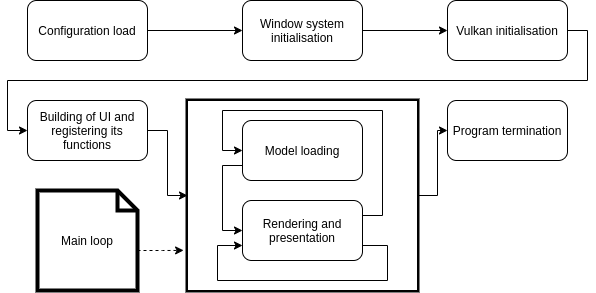
\includegraphics[scale=0.7]{images/program_flow.png}
	\captionsetup{justification=centering}
	\boldcaption[\textbf{Základní rozdělení programu.}]{}
	\label{fig:program_flow}
\end{figure}

\section{Načítání modelů a jejich transformace} \label{sec:voxel_conversion}
Pro vykreslování modelů je nutné je transformovat do octree. Jelikož neexistuje žádný standardní formát pro voxely, je potřeba implementovat import pro různé formáty. Aplikace je prozatím schopna importovat formát \texttt{vox} (sekce \ref{sec:format})).

Načítání dat je rozděleno na dvě části. V~první části jsou ze vstupního souboru načteny využité materiály a je vytvořen seznam voxelů. Tohle je jediná část, kterou je nutné implementovat speciálně pro nové formáty. Zbytek převodu je popsán v~algoritmu \ref{alg:vox_to_svo}.


\begin{center}
	\begin{czechalgorithm}[H] \label{alg:vox_to_svo}
		voxels.sort() \\
		tree\_depth = calculate\_tree\_depth(voxels)\\
		root = tree.init\_root()\\
		\ForEach{voxel in voxels}{
			node = root\\
			\For{level = 0; level < tree\_depth; level++} {
				index\_for\_level = getIndexForLevel(voxel.position, level, tree\_depth)\\
				child\_node = node.get\_or\_create\_node(index\_for\_level)\\
				// nastaveni hodnot voxelu (material...)\\
				node = child\_node\\
			}
			node.is\_terminal = true\\
		}
		\caption{Převod voxelů do octree}
	\end{czechalgorithm}
\end{center}

Po vytvoření stromové reprezentace je dalším krokem minimalizace stromu. Pokud jsou některé oblasti zaplněné, je možné snížit jeho složitost -- označíme uzel na vyšší úrovni jako terminální a jeho potomky odstraníme.

\begin{center}
	\begin{czechalgorithm}[H] \label{alg:minimize_svo}
		\SetKwFunction{FMinTree}{MinimizeTree}
		\SetKwFunction{FIsFilled}{IsNodeFilled}
		\SetKwProg{Fn}{Function}{:}{}

		\Fn{\FIsFilled{$node$}}{
			\KwRet $node$.child\_count == 8 \&\& all\_of($node$.children, IsFilled)\\
		}

		\Fn{\FMinTree{$node$}}{
			\uIf{IsNodeFilled($node$)}{
				node.children.clear()\\
				node.is\_terminal = true\\
			}
			\uElse{
				\ForEach{child in $node$.children}{
					MinimizeTree(child)\\
				}
			}
		}
		\caption{Minimalizace octree}
	\end{czechalgorithm}
\end{center}

\begin{figure}[H]
	\centering
	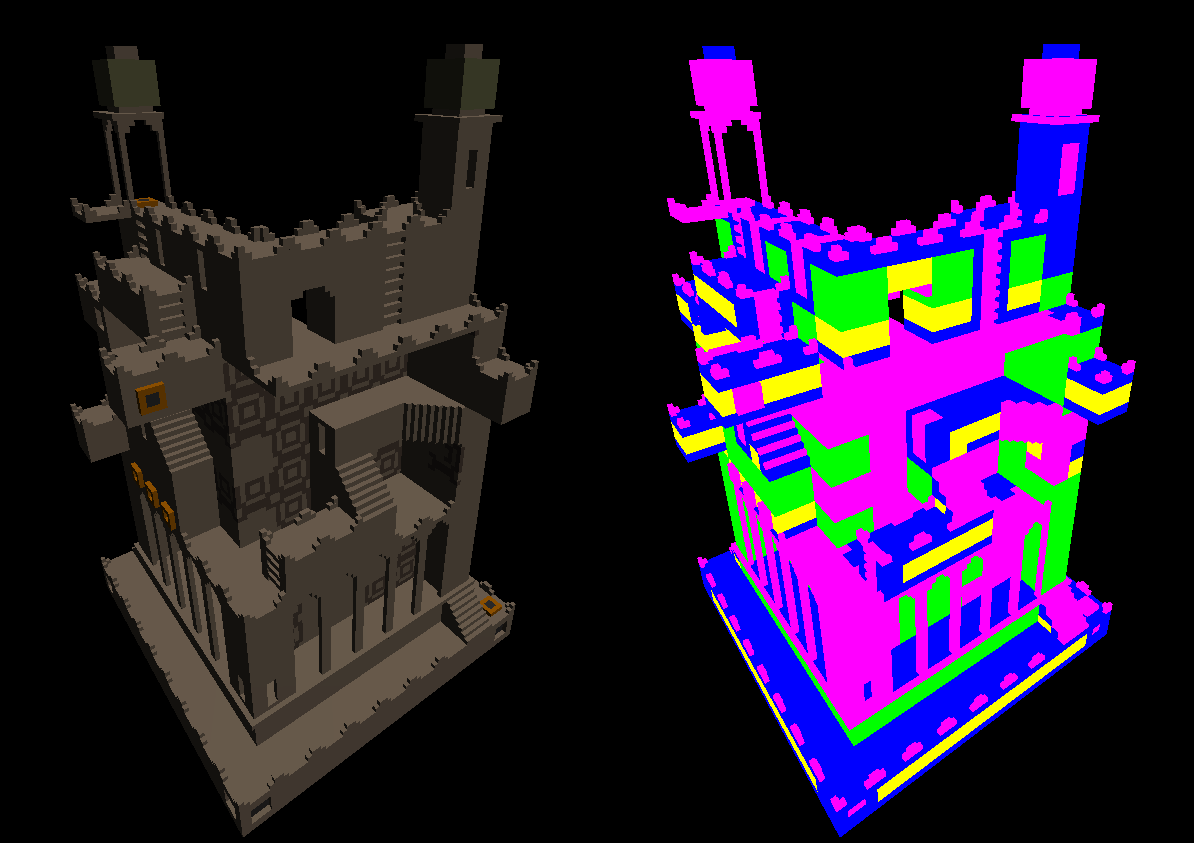
\includegraphics[scale=0.7]{obrazky-figures/levels_render.png}
	\captionsetup{justification=centering}
	\boldcaption[\textbf{Vizualizace hloubky voxelů ve stromu.}]{ Levá část obsahuje render, vpravo jsou barevně odlišené úrovně octree. }
	\label{fig:imgui_classes}
\end{figure}



Finálním krokem je transformace vytvořeného stromu do jeho binární reprezentace popsané v~sekci \ref{sec:voxel_representation}.


\section{Výpočet průsečíku se scénou} \label{sec:bvh_traversal_impl}
Paprsky vycházející z kamery jsou generovány podle rovnice \ref{eq:ray_gen}. $\vec{c}$ značí normalizovanou pozici současného pixelu, $\vec{near}$ určuje pozici blízké roviny (near plane), $\vec{far}$ roviny vzdálené (far plane) a $p$ je výsledný paprsek pro pozici na obrazovce.


\begin{equation} \label{eq:ray_gen}
	\begin{gathered}
	    \vec{c} = calculateNormalizedScreenCoords()\\
	    \vec{near} = inverseProjectionView \cdot <c_{xy}, -1, 1>\\
	    \vec{far} = inverseProjectionView \cdot <c_{xy}, 1, 1>\\
	    \vec{origin} = \frac{near_{xyz}}{near_w}\\
	    \vec{direction} = normalize(\frac{far_{xyz}}{far_w} - origin)\\
	    p = (\vec{origin}, \vec{direction})
	\end{gathered}
\end{equation}

Algoritmus \ref{alg:traverse_bvh_impl} popisuje průchod BVH stromem za využití zásobníku. Důležitou součástí tohoto algoritmu je řazení potomků uzlu podle jejich vzdálenosti od počátku paprsku. Díky tomu jsou uzly stromu procházeny v pořadí od nejbližšího, lze tedy od určité chvíle naprosto ignorovat modely, jejichž obalové těleso (AABB) se nachází dále než prozatím nejbližší průsečík scény. Je zde také menší pravděpodobnost, že bude docházet k větvení kvůli pořadí průchodu.

\begin{center}
	\begin{czechalgorithm}[H] \label{alg:traverse_bvh_impl}
	    \SetKw{Or}{\hspace{\algoskipindent}\itshape or\;}
        \SetKw{And}{\hspace{\algoskipindent}\itshape and\;}
        \SetKw{Not}{\itshape not}
		\SetKwFunction{FTraverseBVH}{TraverseBVH}
		\SetKwFunction{FIntersectNode}{IntersectNode}
		\SetKwProg{Fn}{Function}{:}{}

		\Fn{\FTraverseBVH{$ray$}}{
		    node = root\\
		    stack = EmptyStack()\\
		    calculate intersection with root\\
		    \While{intersected}{
		       \While{intersected \And \Not intersected is leaf}{
		            intersection\_a = IntersectNode(node.left\_child)\\
		            intersection\_b = IntersectNode(node.right\_child)\\
		            swap intersections so that the closer one is in instersection\_a\\
		            \uIf{intersection\_b hit \And intersection\_b is closer than nearest geometry hit}{
		                stack.Push(node.right\_child)
		            }
		            \uIf{neither node hit \And \Not stack.Empty()}{
		                intersection\_a = stack.Pop()
		            }
		        }
		        \uIf{intersected is leaf}{
        		    \uIf{intersection is closer than nearest geometry hit}{
        		        calculate model intersection and save distance if hit
        		    }
        		}
        		\eIf{stack.Empty()}{
        		    intersected = false
        		} {
        		    node = stack.Pop()
        		}
			}
		}
		\caption{Průchod paprsku hierarchií obalových těles}
	\end{czechalgorithm}
\end{center}

\section{Správa modelů} \label{sec:model_management}

Pro modely ve scéně jsou použity tři samostatné struktury. Pro uložení základních informací, jako je transformační matice či obalové těleso, má každý model samostatnou strukturu. Data modelu -- octree a materiály -- jsou uloženy ve dvou bufferech, přičemž jsou tyto buffery sdíleny napříč všemi modely. Informační struktura obsahuje offsety pro umístění dat modelu ve zmíněných bufferech. Rozmístění těchto dat je na obrázku \ref{fig:model_storage}.

\begin{figure}[H]
	\centering
	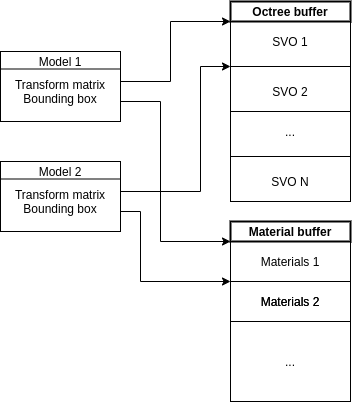
\includegraphics[scale=0.7]{images/model_storage.png}
	\captionsetup{justification=centering}
	\boldcaption[\textbf{Informace o modelu a vztahy k datovým bufferům.}]{ }
	\label{fig:model_storage}
\end{figure}

Pro usnadnění práce s alokací GPU paměti byla vytvořena třída \texttt{BufferMemoryPool}, která spravuje předaný buffer. Třída umožňuje zvolit zarovnání bloků při propůjčení paměti a zaručuje, že nedojde k přepisu již zapůjčených dat. Zapůjčené paměťové bloky využívají RAII\footnote{\url{https://en.cppreference.com/w/cpp/language/raii}} ke znemožnění úniku paměti.  Ukázka použití této třídy je ve výpisu \ref{lst:memory_pool}.

\begin{lstlisting}[label={lst:memory_pool}, language=C++, caption={Ukázka využití memory pool}]
auto buffer = createBuffer(100_MB);
auto memoryPool = BufferMemoryPool{buffer, ALIGNMENT};

auto memoryBlock = memoryPool.leaseMemory(2_MB);
modelInfo.setMemoryOffset(memoryBlock.getOffset());
memoryBlock.mapping().set(data);
// ...
memoryPool.returnMemory(memoryBlock);
\end{lstlisting}

Celý proces načtení nového modelu z disku je popsán v obrázku \ref{fig:load_model_diagram}. Program umožňuje načítat dva typy formátů -- \texttt{VOX}, jehož data je nutné transformovat do octree a \texttt{PF\_VOX}, jež má již vhodnou podobu. Po načtení dochází k alokaci grafické paměti a odeslání dat do ní. Finálním krokem je aktualizace hierarchie obalových těles.

\begin{figure}[H]
	\centering
	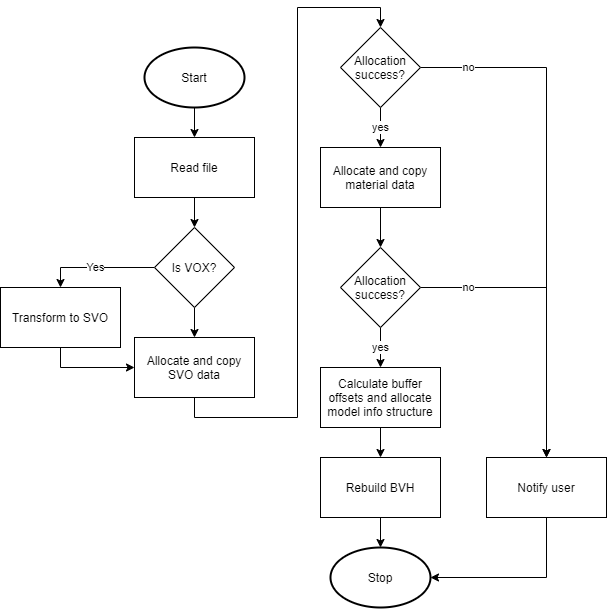
\includegraphics[scale=0.7]{images/load_diagram.png}
	\captionsetup{justification=centering}
	\boldcaption[\textbf{Diagram načítání dat modelů.}]{ }
	\label{fig:load_model_diagram}
\end{figure}

\subsection{Načítání a ukládání scén}
Pro účel zjednodušení práce s modely aplikace podporuje jednoduchý konfigurační soubor pro uložení rozložení scény. Formátem tohoto souboru je \texttt{TOML}, podobně jako u konfiguračního souboru aplikace. Soubor definice scény je rozdělen na dvě části.

První částí je definice pozice a rozložení pole sond (light field probes). Položka \texttt{probeGridPos} určuje pozici počátku mřížky sond a \texttt{probeGridStep} definuje vzdálenost jednotlivých sond. \texttt{proximityGridSize} určuje rozdělení prostoru pokrytým sondami na voxely, které obsahují informace o sondách pro tento podprostor nejvhodnějších.

Další částí je pole modelů ve scéně obsažených. Záznamy modelů obsahují cestu k souboru pro načtení dat modelu a také vektory k jeho transformaci.

Ukázka jednoduchého souboru scény je ve výpisu \ref{lst:scene_config}.\\\\

\begin{lstlisting}[label={lst:scene_config}, language=toml, caption={Definice jednoduché scény}]
probeGridPos = [ -1.0, 0.0, -1.0 ]
probeGridStep = 1.5
proximityGridSize = [ 64, 64, 64 ]

[[models]]
path = '/chair.vox'
rotateVec = [ 0.0, 0.0, 0.0 ]
scaleVec = [ 4.0, 4.0, 4.0 ]
translateVec = [ 0.0, 0.0, 0.0 ]
\end{lstlisting}

V implementaci je i téměř dokončená logika pro načítání scén připravených pro hru Teardown. Modely ve formátu, které hra využívá, jsou na nejnižší úrovni ve \texttt{VOX} souborech. Definice scény je v samostatném \texttt{XML} souboru, který určuje transformace modelů a umožňuje definovat objekty "otexturované" jiným modelem.

\section{Demonstrační aplikace}\label{sec:demo_app}
Demonstrační aplikace slouží k vizualizaci výsledků a práci s modely/scénami. Aplikace může pracovat ve dvou režimech:
\begin{itemize}
    \item Editační režim -- v tomto režimu je scéna vykreslována pouze pomocí sparse voxel octree ray marchingu a slouží primárně k vytvoření scény a jejímu uložení na disk. Také je zde možné sledovat stav sond.
    \item Renderovací režim -- slouží k načítání scén vytvořených v předchozím režimu a demonstraci výsledného algoritmu.
\end{itemize}

Uživatelské rozhraní je implementováno pomocí knihovny \texttt{pf\_imgui} představené v sekci \ref{sec:pf_imgui}. Většina prvků uživatelského rozhraní obsahuje tooltipy pro snadné zjištění funkce jednotlivých komponent a UI okna lze přetáhnout ven z hlavního okna pro lepší přehlednost. Bližší popis se nachází na přiloženém paměťovém médiu, základní přehled zde ale bude uveden.

UI aplikace je rozděleno do následujících částí:

\begin{itemize}
	\item Info -- zobrazení statistik vykreslování (počet snímků za sekundu, flame graph), informace o~kameře a její parametry, a také informace o právě vykreslované scéně.
	\item Render settings -- výběr typu zobrazení (stínování, normály, počet iterací, hloubka ve~stromě...), ovládání světla.
	\item Debug -- memo pro výstup logů, připravený Chaiscript pro přidávání složitějších funkcí.
	\item Debug images -- okno pro zobrazení textury reprezentující počet iterací při průchodu octree.
	\item Shader controls -- ovládání parametrů pro shadery.
	\item Probe grid controls -- ovládání mřížky sond.
	\item Models -- ovládání modelů zobrazených ve scéně.
	\item Probes info -- vizualizace atlasu sond a renderování scény pomocí něj.
\end{itemize}


\begin{figure}[H]
	\centering
	\captionsetup{justification=centering}
	\begin{subfigure}[t]{.49\textwidth}
		\centering
		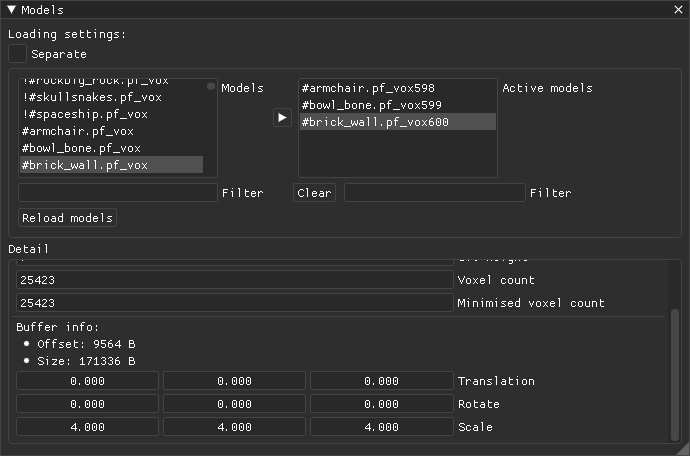
\includegraphics[scale=1]{images/dp_ui_models.png}
		\caption{\textbf{Okno pro přidávání a manipulaci s modely}}
		\label{fig:model_ui}
	\end{subfigure}
		\begin{subfigure}[t]{.49\textwidth}
		\centering
		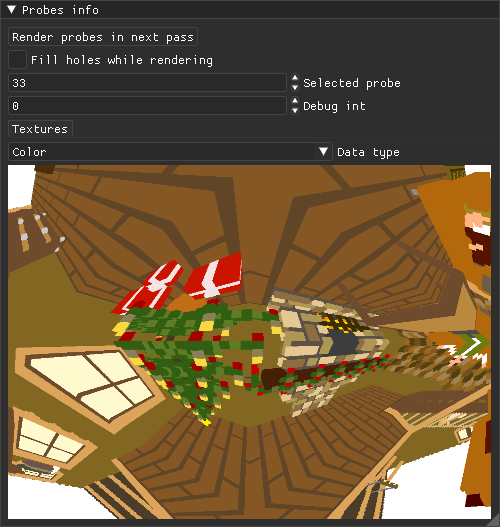
\includegraphics[scale=1]{images/dp_ui_probes.png}
		\caption{\textbf{Okno pro zobrazení atlasu textur sond}}
		\label{fig:probe_ui}
	\end{subfigure}
		\begin{subfigure}[t]{1\textwidth}
			\centering
        	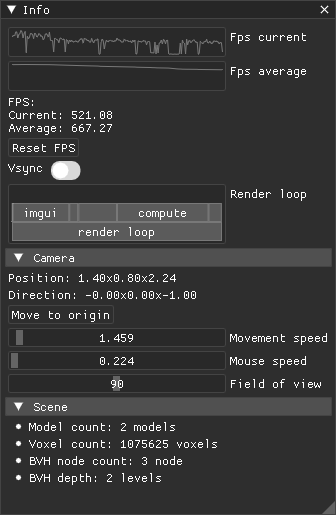
\includegraphics[scale=1]{images/dp_ui_info.png}
        	\caption{\textbf{Informační okno}}
        	\label{fig:info_ui}
	\end{subfigure}\\
	\captionsetup{justification=centering}
	\boldcaption[\textbf{Ukázka oken demonstrační aplikace.}]{ }
	\label{fig:UI}
\end{figure}


\subsubsection{Konfigurace}
Důležitou součástí aplikace je konfigurační soubor, který je blíže popsán v příloze \ref{appendix:configfile}. Tento soubor obsahuje primárně informace o cestách ke zdrojům (cesta k modelům, shaderům...). Také je v něm obsažena definice velikosti okna demonstrační aplikace a velikost pracovní skupiny pro vykreslování za pomoci octree. Aplikace automaticky ukládá data, která uživatel nastavil v uživatelském rozhraní.

Typ souboru zvolený pro konfiguraci je \texttt{TOML}. Tento formát byl zvolen primárně z toho důvodu, že je velice snadno čitelný pro uživatele a není tedy nutné vytvářet separátní program pro manipulaci s konfigurací. Samozřejmě existují podobné, uživatelsky přívětivé formáty, jako například \texttt{YAML} nebo \texttt{INI}, ale \texttt{TOML} byl zvolen také kvůli knihovně \texttt{toml++}, díky které je manipulace s konfiguračním souborem relativně pohodlná. 


\chapter{Vyhodnocení}
\label{testovani}
V~této kapitole je krátký popis dosažených výsledků týkající se doby převodu vstupních dat a také analýza využití paměti na grafické kartě. Poslední sekce se zabývá grafickými výstupy implementace. Pro měření byla použita následující PC konfigurace:
\begin{itemize}
    \item CPU: AMD Ryzen 5 3600, 6-core, 4.2 GHz.
    \item GPU: ASUS GeForce ROG STRIX RTX 2070S. 
\end{itemize}

\section{Převod vstupních dat na octree}
Převod vstupních dat na octree byl popsán v~sekci \ref{sec:voxel_conversion}. Převod je prozatím prováděn sekvenčně na jednom vlákně, ale v~budoucí verzi jej autor plánuje předělat tak, aby využíval více vláken procesoru. Na obrázku \ref{fig:time_convert} je graf závislosti času převodu na počtu vstupních voxelů. Graf \ref{fig:time_convert_mini} zobrazuje stejné měření s~aktivovanou minimalizací. Měření byla prováděna s~nejvyšší úrovní optimalizací kompilace. Pro měření bylo použito CPU \texttt{Ryzen 3600} a probíhalo na jednom vláknu za využití knihovny \texttt{nanobench}\footnote{\url{https://github.com/martinus/nanobench}}. Model, který byl v~testech použit, byly plné koule o~různých poloměrech.


\begin{figure}[H]
	\begin{subfigure}{.5\textwidth}
		\begin{tikzpicture}[scale=0.7, transform shape]
			\begin{axis}[
				xlabel={velikost scény [voxely]},
				y unit = s,
				ylabel={doba zpracování},
				grid=both
				]
				\addplot table [x=size, y=time, mark=none, color=red]{data/time_convert.txt};
			\end{axis}
		\end{tikzpicture}
		\caption{\textbf{Bez minimalizace}}
		\label{fig:time_convert}
	\end{subfigure}
	\begin{subfigure}{.5\textwidth}
		\begin{tikzpicture}[scale=0.7, transform shape]
			\begin{axis}[
				xlabel={velikost scény [voxely]},
				y unit = s,
				ylabel={doba zpracování},
				grid=both
				]
				\addplot table [x=size, y=time, mark=none, color=red]{data/time_convert_mini.txt};
			\end{axis}
		\end{tikzpicture}
		\caption{\textbf{S~minimalizací}}
		\label{fig:time_convert_mini}
	\end{subfigure}
	\captionsetup{justification=centering}
	\boldcaption[\textbf{Doba tvorby octree.}]{ }
\end{figure}

I~když to není z~grafu příliš znatelné, transformace s~minimalizací je o~několik procent rychlejší, jelikož není nutné vytvářet tak velký finální strom. Pokud by vstupní data byla pro minimalizaci nepříznivá, byla by tato metoda pomalejší.

\section{Paměťová náročnost}
V této sekci je popsána paměťová náročnost dvou hlavních částí částí programu. Jedná se o vyhodnocení využití VRAM.

\subsubsection{Octree}

Každý uzel octree zabírá v~prvé řadě 4 bajty (15 bitů \texttt{child pointer} + 1 bit \texttt{far} + 8 bitů \texttt{valid mask} + 8bitů \texttt{leaf mask}). Dále pro dohledání materiálů a ostatních parametrů další 4 bajty (24 bitů \texttt{value pointer} + 8 bitů \texttt{mask}). Tyto dva záznamy nejsou vytvářeny pro listové uzly. Pokud budeme předpokládat strom, který má prostor obsazený přesně z~50 \% a je obsazen pouze každý druhý voxel, s~hloubkou stromu 6 -- tedy 37448 voxelů -- celková obsazená paměť zmíněnými záznamy bude 18724 bajtů. Při popsaném rozložení voxelů se samozřejmě jedná o~nejhorší možný případ.

\begin{table}[H]
	\centering
	\begin{tabular}{|r|r|}
		\hline
		\multicolumn{1}{|c|}{hloubka stromu} & \multicolumn{1}{c|}{obsazená paměť {[}B{]}} \\ \hline
		1                                    & 4                                           \\ \hline
		2                                    & 36                                          \\ \hline
		3                                    & 292                                         \\ \hline
		4                                    & 2340                                        \\ \hline
		5                                    & 18724                                       \\ \hline
		6                                    & 149796                                      \\ \hline
	\end{tabular}
	\captionsetup{justification=centering}
	\boldcaption[\textbf{Využití paměti podle hloubky stromu při maximální nepříznivosti podmínek.}]{ }
\end{table}

Tímto jsou pokryta základní data popisující strom a vyhledávací strukturu do parametrů. Další paměť je využita \texttt{far} pointery. V~pesimistickém případě je může potřebovat \textasciitilde5 \% uzlů, ovšem jsou potřeba až pro hloubku stromu vyšší než 7, a to kvůli množství potomků v~úrovni.

Poslední data vyžadující velké množství paměti jsou samotné parametry voxelů. Samozřejmě záleží na využitých parametrech, pro phongovo stínování je dostačující barva, tedy 4 bajty (RGBA formát, kde je každý kanál reprezentován 8 bity). Samozřejmě se data dají zakódovat efektivněji.

Celková paměťová náročnost pro octree se zmíněnými parametry je tedy:

\begin{table}[H]
	\centering
	\begin{tabular}{|r|r|}
		\hline
		\multicolumn{1}{|c|}{hloubka stromu} & \multicolumn{1}{c|}{využití paměti {[}B{]}} \\ \hline
		1                                    & 20                                          \\ \hline
		2                                    & 164                                         \\ \hline
		3                                    & 1316                                        \\ \hline
		4                                    & 10532                                       \\ \hline
		5                                    & 84260                                       \\ \hline
		6                                    & 674084                                      \\ \hline
	\end{tabular}
	\captionsetup{justification=centering}
	\boldcaption[\textbf{Využití paměti podle hloubky stromu při využití barevných parametrů pro voxely.}]{ }
\end{table}

Ve všech případech se jedná o~nejhorší možný případ. Realisticky použitelné modely mají paměťovou náročnost výrazně nižší a také u~nich dochází k~minimalizaci stromu (která v~uvažovaném nejhorším případě není možná).


\subsubsection{Light field probes}
Jak bylo zmíněno v sekci \ref{sec:lfp_design}, každá sonda sestává ze dvou textur. První z nich má rozlišení 1024x1024 s datovým typem \texttt{RG32F}, tedy využívá 8 bajtů paměti. Z těchto 8 bajtů jsou 4 využity pro radianci/nepřímé osvětlení, 2 pro normály a 2 pro hloubku. Druhá textura má $\frac{1}{16}$ rozlišení hlavní textury a obsahuje pouze informace o hloubce. Datovým typem této textury je \texttt{R16F}, což znamená, že každý texel zabírá 2 bajty. Využití paměti jedné sondy je tedy 8396800 bajtů (\textasciitilde{}8.4 MB).

Samozřejmě není použita jen jedna sonda. Množství sond je kvůli implementaci algoritmů s nimi pracujících omezeno na mocniny dvou v každé ose. V následující tabulce je seznam využití paměti pro množství sond, které se nejpravděpodobněji využijí.

\begin{table}[H]
	\centering
    \begin{tabular}{|l|l|}
    \hline
    počet sond & využití paměti {[}MB{]} \\ \hline
    1          & 8.4                     \\ \hline
    4          & 33.5                    \\ \hline
    16         & 134.3                   \\ \hline
    128        & 1074.8                  \\ \hline
    512        & 4299.1                  \\ \hline
    \end{tabular}
	\captionsetup{justification=centering}
	\boldcaption[\textbf{Využití paměti pro časté velikosti mřížky.}]{ }
\end{table}


\section{Výsledky}

\begin{figure}[H]
	\centering
	\captionsetup{justification=centering}
	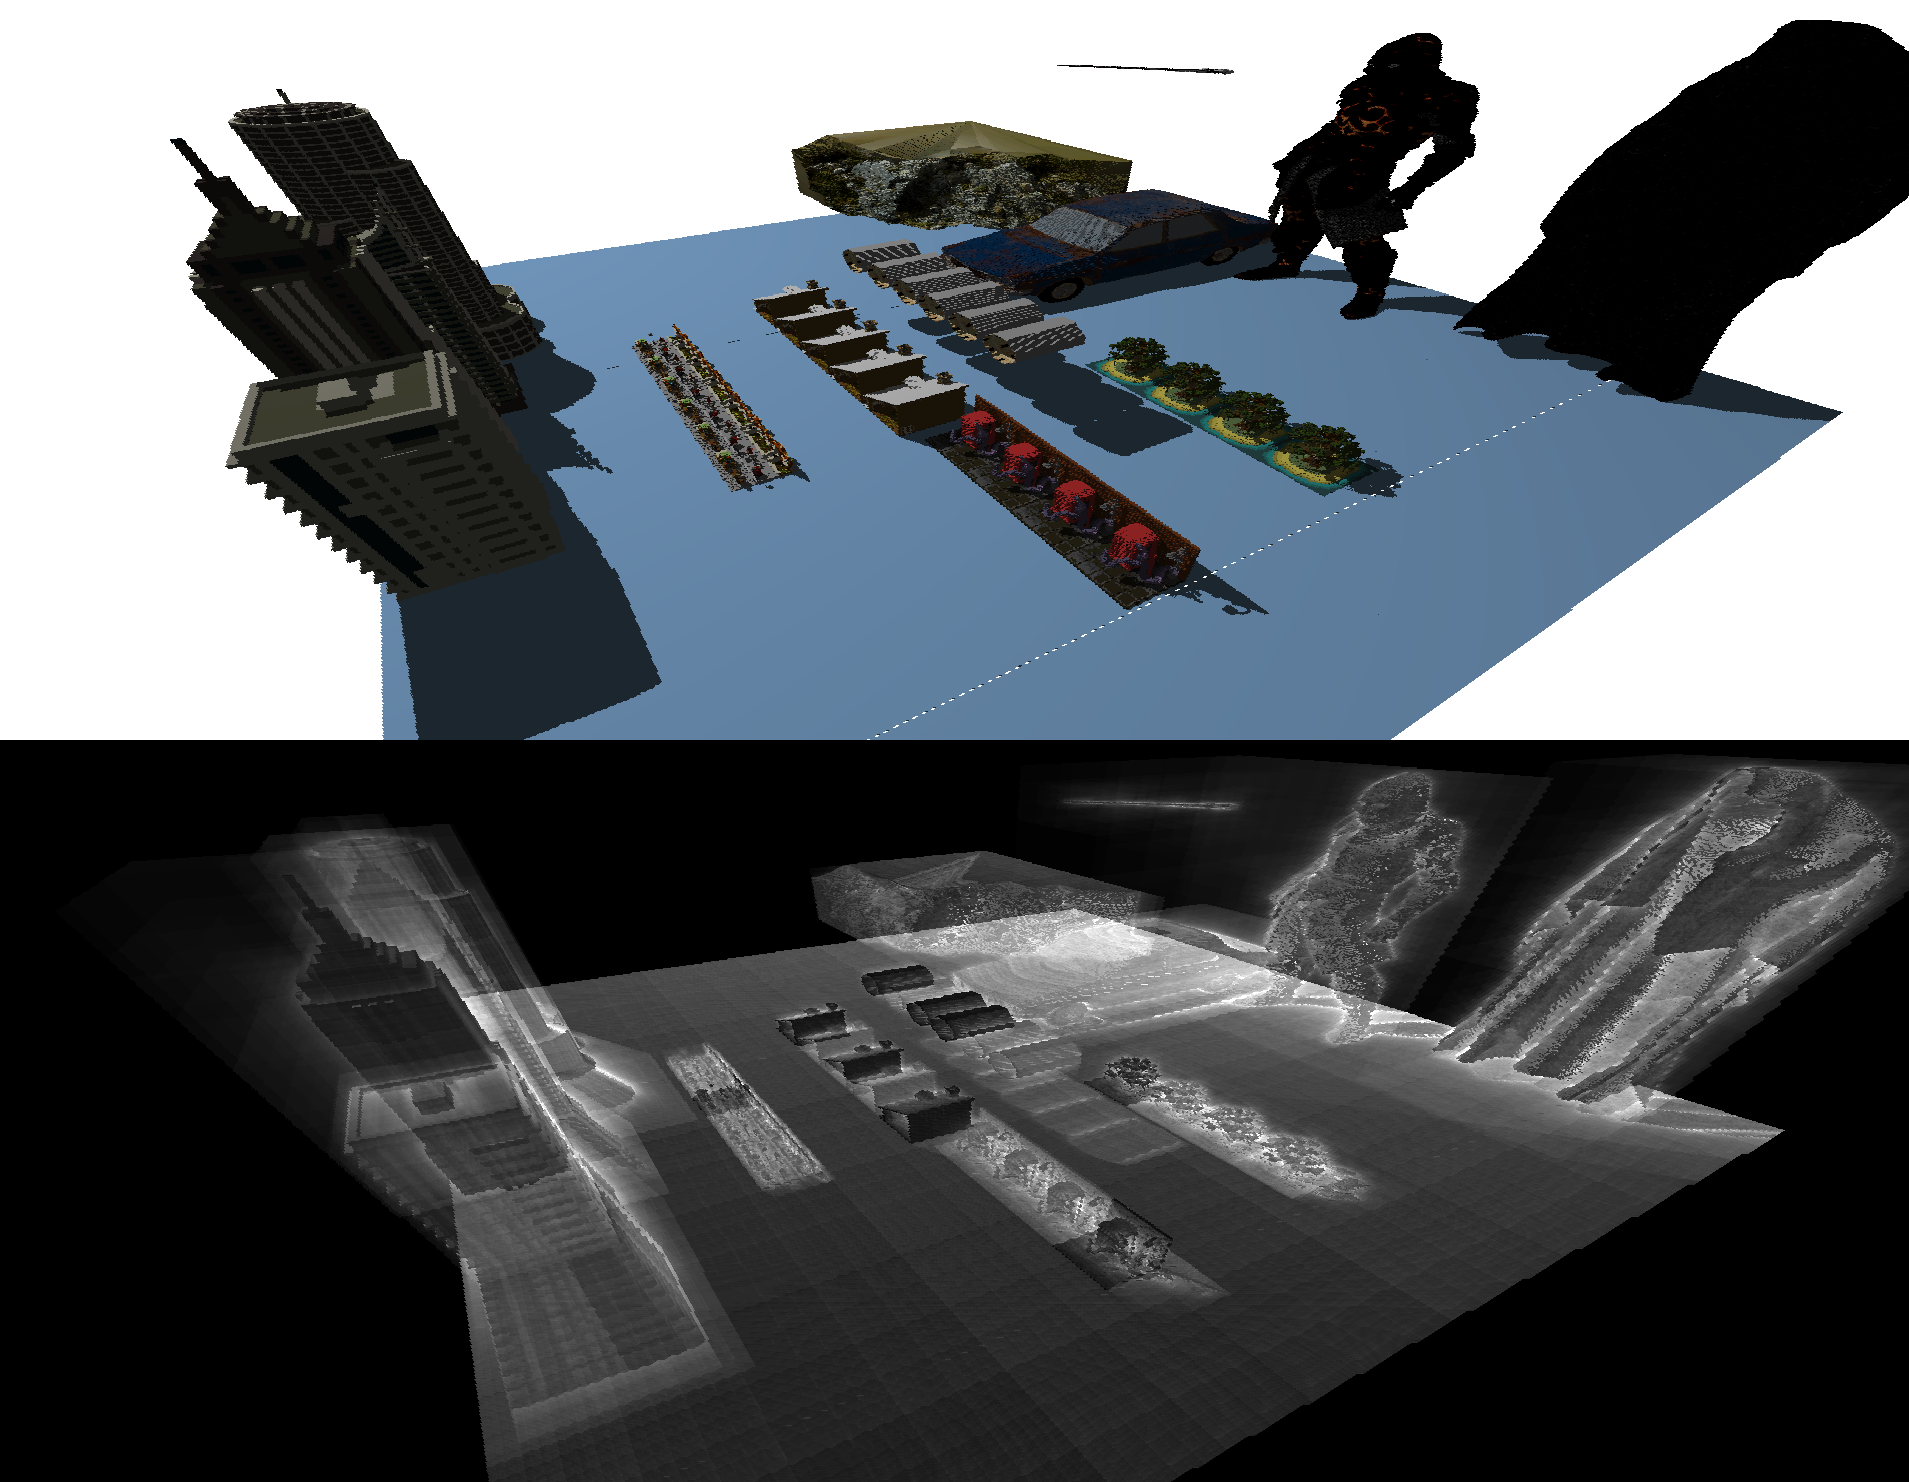
\includegraphics[scale=0.2]{images/12M_scene.png}
	\boldcaption[\textbf{Scéna vykreslena pomocí sparse voxel octree ray tracing.}]{ V horní části obrázku se nachází vykreslená scéna se stíny, v dolní části je počet iterací nutný k výpočtu hodnot jednotlivých pixelů -- bílá barva v tomto případě znamená 200 iterací.}
	\label{fig:12M_render}
\end{figure}


Na obrázku \ref{fig:12M_render} je vykreslena scéna pomocí sparse voxel octree ray tracing. Scéna obsahuje 36 modelů složených z 12-ti milionů voxelů. Hierarchie obalových těles této scény obsahuje 71 uzlů, má tedy hloubku 7 úrovní. Nejvyšší počet iterací nutných k výpočtu průsečíku zde bylo \textasciitilde{}200 iterací (kroků průchodu stromu). Ve scéně je prováděn výpočet ostrých stínů. Na hardware, který byl zmíněn na začátku kapitoly, a při rozlišení 1920x1080 pixelů byla tato scéna vykreslena rychlostí 100 snímků za sekundu. Při vypnutí paprsků pro stíny došlo ke zrychlení o 20\%, tedy 120 snímků za sekundu. Samozřejmě na snímku dochází k nejhoršímu možnému případu -- všechny modely jsou viditelné a plocha, která je naspod, je velice neefektivní, jelikož se jedná o velký model, který má výšku pouze jednoho voxelu. Dělba prostoru pomocí octree je v tomto případě poněkud neefektivní.  Po jeho odstranění dojde ke zrychlení na 300 snímků za sekundu. 

\begin{figure}[H]
	\centering
	\captionsetup{justification=centering}
	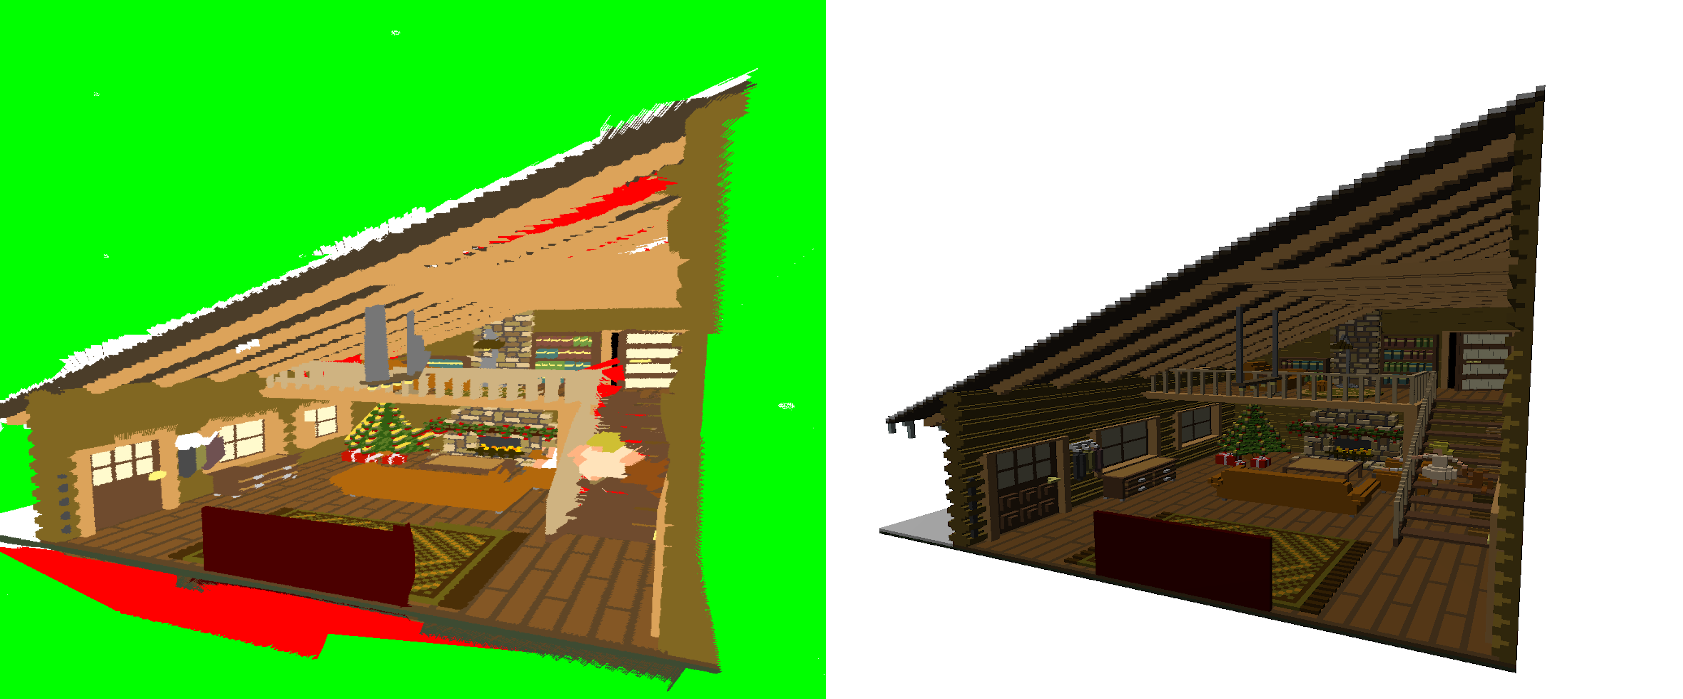
\includegraphics[scale=1]{images/render_probe_vs_svo.png}
	\boldcaption[\textbf{Srovnání scény vykreslené pomocí light field probes a sparse voxel octree.}]{ V levé části obrázku je scéna vykreslena pomocí light field probe ray tracing. Zelené oblasti zobrazují minutí scény, červené nemožnost zjistit výsledek pro paprsek. Pravá část je stejná scéna vykreslena pomocí sparse voxel octree.}
	\label{fig:probe_vs_svo_render}
\end{figure}

Obrázek \ref{fig:probe_vs_svo_render} obsahuje porovnání vykreslení scény z pohledu kamery pomocí light field probe ray tracing a sparse voxel octree ray tracing. Z obrázku je jasně vidět, že metoda není vhodná jako primární vykreslovací algoritmus. Výsledek obsahuje spoustu pixelů, kde nebyl nalezen výsledek a dochází k mnoha nepřesnostem, jak je lépe vidět na obrázku \ref{fig:probes_inaccuracy}.

\begin{figure}[H]
	\centering
	\captionsetup{justification=centering}
	
\includegraphics[scale=2.5]{images/probes_inaccuracy.png}
	\boldcaption[\textbf{Přiblížení na artefakty light field probes ray tracing.}]{}
	\label{fig:probes_inaccuracy}
\end{figure}

Jak bylo popsáno v sekci \ref{sec:indirect}, namísto radiance zobrazené výše je v sondách vykreslen příspěvek nepřímého osvětlení. Obrázek \ref{fig:probes_indirect_scene} zobrazuje nepřímé osvětlení ve scéně.

\begin{figure}[H]
	\centering
	\captionsetup{justification=centering}
	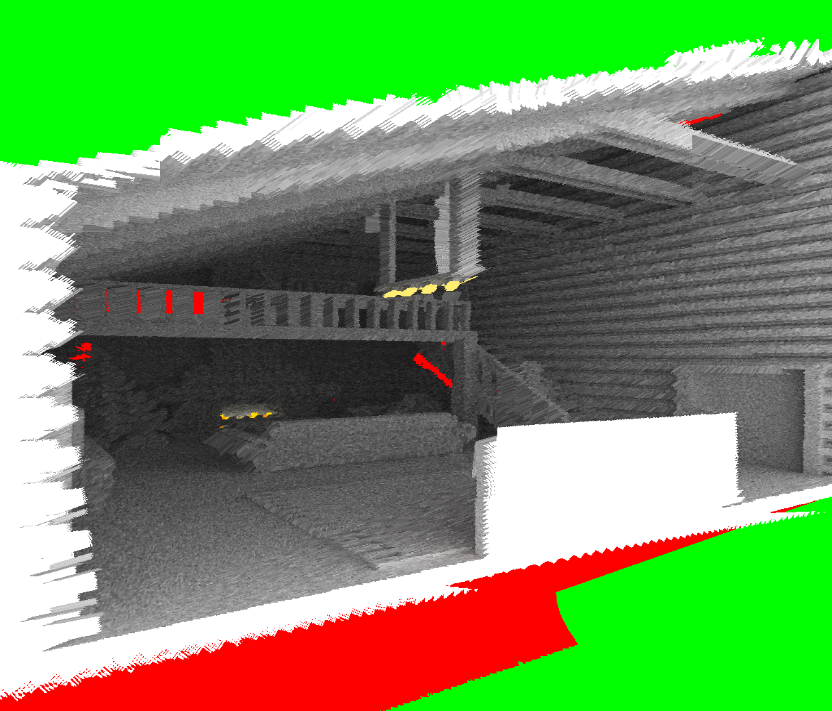
\includegraphics[scale=1]{images/probe_indirect_render.png}
	\boldcaption[\textbf{Scéna vykreslena pomocí light field probes s nepřímým osvětlením.}]{}
	\label{fig:probes_indirect_scene}
\end{figure}

Při kombinaci zmíněných algoritmů je vykreslena scéna pomocí sparse voxel octree a ze sond je získáno nepřímé osvětlení. Výsledek je na obrázku \ref{fig:render_indirect_1}. Z obrázku je vidět, že ne u všech fragmentů došlo k úspěšnému dohledání hodnot pro nepřímé osvětlení. Důvodem jsou dříve zmíněná "neviditelná" místa, kdy žádná z kandidátních sond "nevidí" na pozici.

\begin{figure}[H]
	\centering
	\captionsetup{justification=centering}
	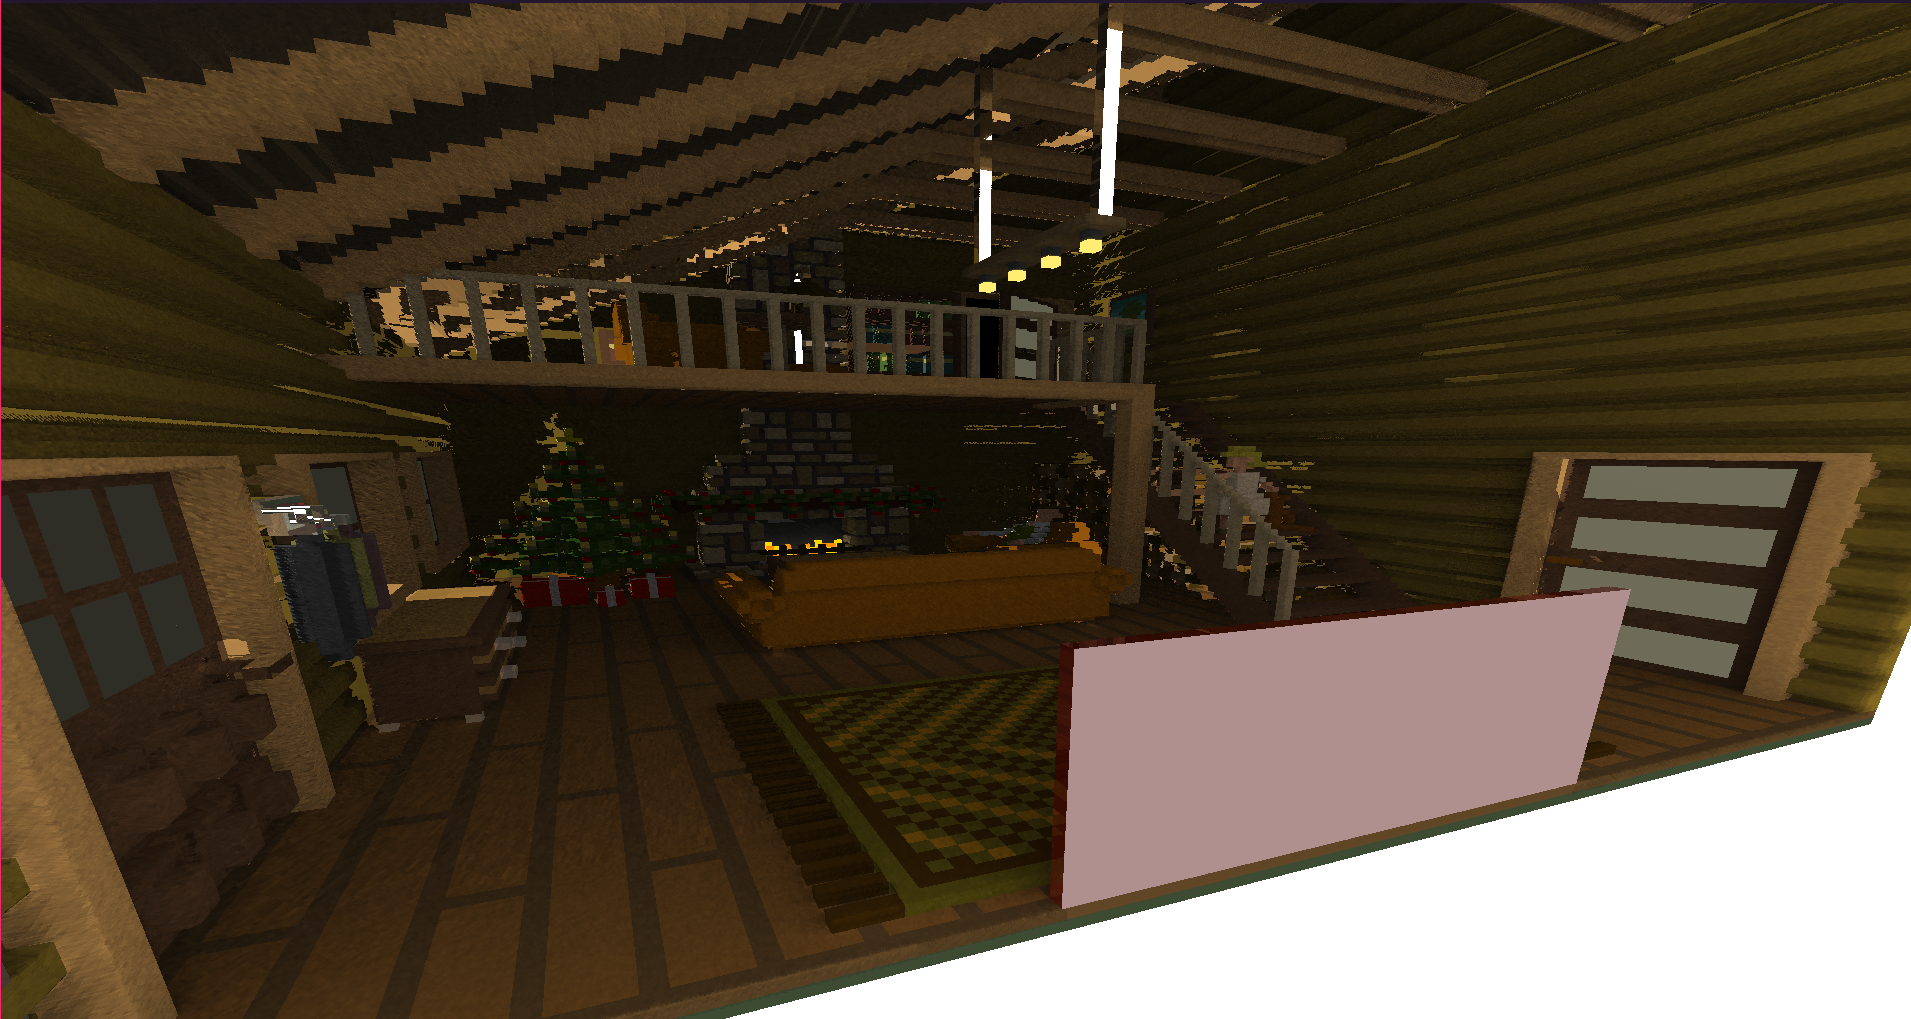
\includegraphics[scale=0.9]{images/render_svo_indirect_1.png}
	\boldcaption[\textbf{Scéna vykreslena kombinací light field probes a sparse voxel octree.}]{}
	\label{fig:render_indirect_1}
\end{figure}

Tento přístup je tedy vhodnější pro scény, kde nedochází k častému překryvu, jako ve scéně výše. Na obrázku \ref{fig:tree_closeup} je bližší snímek vánočního stromu z obrázku \ref{fig:render_indirect_1}. Žádná ze sond na toto místo nevidí a vznikají tím nehezké artefakty. Je možné pokusit se zakrýt tyto problémy čtením dat ze sondy pouze ve směru místa průsečíku namísto přesné vzdálenosti, to ale přináší podobné problémy. 

\begin{figure}[H]
	\centering
	\captionsetup{justification=centering}
	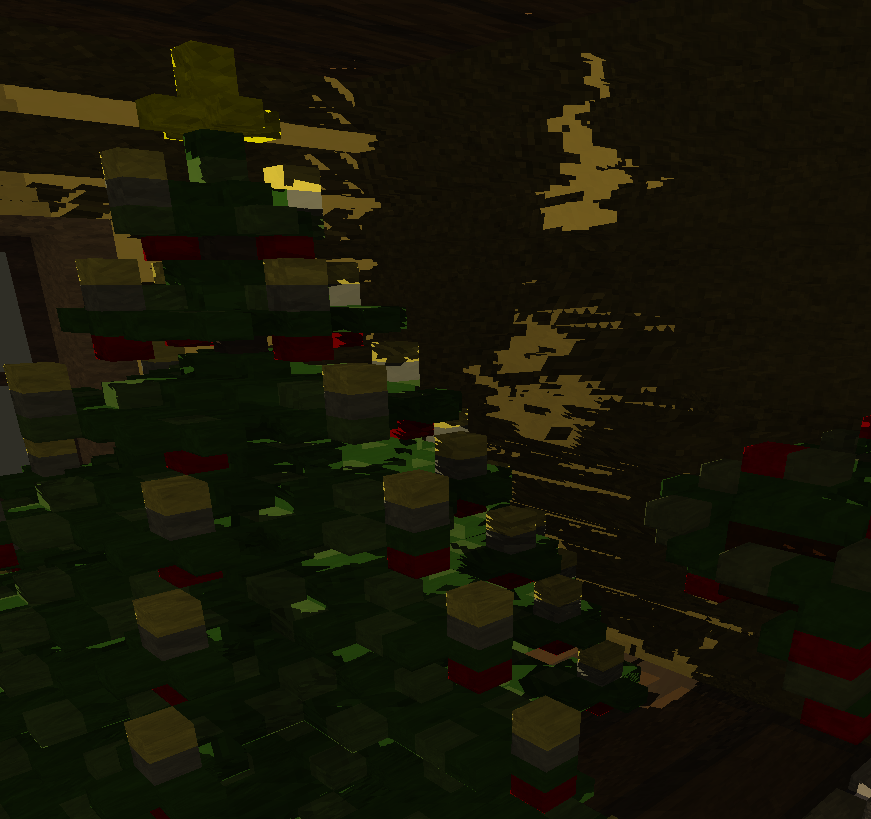
\includegraphics[scale=1.15]{images/tree_closeup.png}
	\boldcaption[\textbf{Artefakty v prostoru kde sonda "nevidí".}]{}
	\label{fig:tree_closeup}
\end{figure}


\begin{figure}[H]
	\centering
	\captionsetup{justification=centering}
	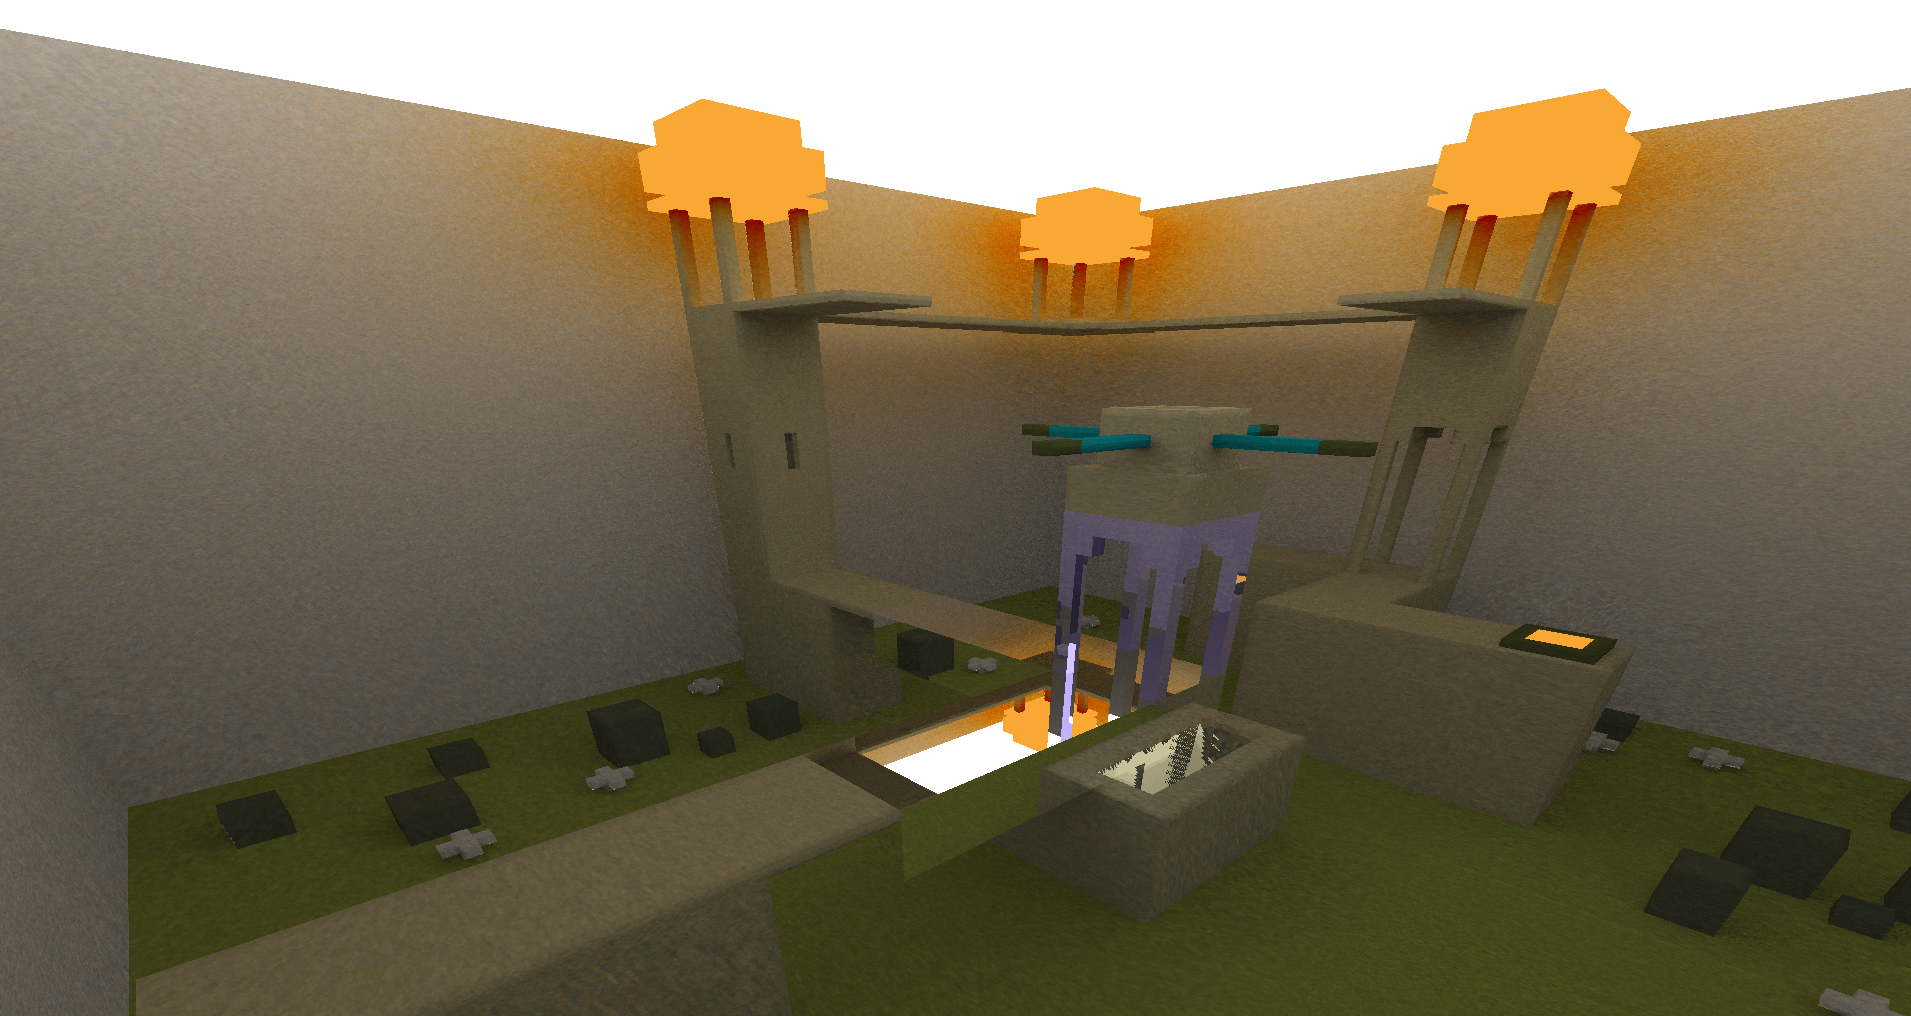
\includegraphics[scale=0.9]{images/indirect_render_2.png}
	\boldcaption[\textbf{Ukázka scény s emisivním a reflektivním materiálem.}]{Oranžové objekty jsou zdroji světla. Ve středu spodní části obrázku se nachází reflektivní materiál. Ve scéně se nenachází zdaleka tolik artefaktů jako v té předchozí díky její jednoduchosti.}
	\label{fig:indirect_render_2}
\end{figure}


\chapter{Závěr}\label{zaver}
Cílem práce bylo navrhnout systém pro zobrazování voxelových modelů v reálném čase za využití GPU akcelerace a implementovat ho. K dosažení tohoto cíle bylo nejdříve nutné si nastudovat již existující algoritmy řešící podobné problémy. Algoritmů pro realistické vykreslování existuje poměrně hodně, některé z nich byly představeny v první kapitole. Bylo také nutné se seznámit s možnostmi reprezentace voxelových dat a možné interakce s nimi -- například výpočet průsečíku. V neposlední řadě bylo potřeba představit užitečné datové struktury pro dělbu prostoru, díky kterým je možné optimalizovat různé algoritmy.

Následný návrh se zabýval specifickou reprezentací voxelových dat k možnosti efektivního nalezení průsečíku s paprskem. Metoda reprezentace těchto dat byla založena na článku \cite{Laine2011EfficientSV}. Jako způsob uložení voxelových dat byla navržena úsporná struktura sparse voxel octree. Dále zde byly představeny některé metody pro vykreslování scén. První z nich je založena na sledování paprsku ve výše zmíněné datové struktuře, přičemž bylo navrženo rozšíření využívající hierarchie obalových těles ke snazší práci s modely a urychlení jejich vykreslování. Dalším důležitým zdrojem byl článek \cite{light_field_probes}, který představil koncept light field probes. V návrhu byl popsán způsob reprezentace dat sond za pomocí atlasu textur obsahující informace pro možnost sledování paprsku skrze tyto struktury. Byla vysvětlena též zmíněná metoda pro vykreslování a vlastní optimalizace za použití voxelového pole, která umožňuje algoritmus zrychlit a zlepšuje jeho úspěšnost pro nalezení průsečíku se scénou. Pro přípravu nepřímého osvětlení scény byla navržena metoda založena na light field probes, která využívá atlasu textur k uložení dat o nepřímém osvětlení -- tato data lze využít v dalším algoritmu. Byla též popsána struktura výsledného vykreslovacího řetězce, která byla rozdělena na samotné vykreslení scény a aplikace nepřímého osvětlení ze sond.

Pro implementaci aplikace bylo využito API Vulkan společně s mnoha dalšími knihovnami zmíněnými v kapitole \ref{implementace}. V průběhu implementace návrhu vznikly tři knihovny, které byly krátce popsány. Specificky se týkaly obecné funkčnosti, práce s okny a grafickou kartou a uživatelského rozhraní. Kapitola specifikovala některé zajímavé části implementace, jako je budování octree pro modely a správa modelů uvnitř programu.

Výsledná demonstrační aplikace umožňuje uživateli vytvořit si vlastní scénu, či nahrát již scény připravené. Demonstruje funkčnost sparse voxel octree ray tracing, pro který zobrazuje i informace pro evaluaci scény, a také light field probes, kdy je možné zkoumat obsah jednotlivých sond. V alternativním režimu vykresluje scény kombinací těchto dvou algoritmů.

Z pohledu efektivity algoritmů je načítání scén poměrně pomalé, díky implementaci vlastního formátu je ale možné tomuto zpomalení předejít. Náročnost algoritmů na paměť je pro reprezentaci voxelových modelů poměrně přijatelná, lze vykreslovat scény o velikosti desítek milionů voxelů s využitím paměti, se kterou by neměly problémy ani starší grafické karty. Paměťová náročnost sond je poněkud vyšší, realistické využití s dalšími strukturami je pro maximální velikost mřížky sond přibližně 8x8x8. Paměťové omezení dané sondami implikuje, že navržený systém je vhodnější spíše pro scény v menší škále, ovšem s vysokou úrovní detailu.

Výsledné grafické výstupy tedy mohou obsahovat rozsáhlé scény, dochází ovšem ke vzniku artefaktů. Tyto artefakty jsou poměrně rušivé a s využitím použitých metod jim pravděpodobně nelze předejít. Alternativou k použitému přístupu by mohla být metoda uvedena v článku \textit{Dynamic Diffuse Global Illumination with Ray-Traced Irradiance Fields}, která navíc umožňuje využívat dynamických scén, na rozdíl od metody použité zde, která zvládá pouze scény statické. Mezi další rozšíření by mohla patři implementace anti-aliasingu, specificky nějaká temporální metoda by byla zajímavá. Dalším vhodným rozšířením by byla implementace datové struktury, která by umožňovala optimalizované streamování dat scény z disku, aby bylo možné zobrazovat rozsáhlé scény bez nutnosti čekat na načtení modelů. 



%===============================================================================
